\documentclass[titlepage,12pt,a4paper,ngerman]{report}
\usepackage[utf8]{inputenc}
\usepackage[T1]{fontenc}
\usepackage[german]{babel}
\usepackage{graphicx}
\usepackage{wrapfig}
\usepackage{amsmath}
\usepackage{cleveref}
\usepackage{amsfonts}
\usepackage{amssymb}
\usepackage{tikz}
\usepackage{nicefrac}
\usepackage{mathtools}
\usepackage[margin=1in]{geometry}
\usepackage{enumerate}
\usepackage{tocloft}

\addtolength{\cftchapnumwidth}{10pt}
\addtolength{\cftsecnumwidth}{10pt}
\addtolength{\cftsubsecnumwidth}{10pt}

\newcommand{\verteq}{\rotatebox{90}{$\,=$}}
\newcommand{\equalto}[2]{\underset{\scriptstyle\overset{\mkern4mu\verteq}{#2}}{#1}}
\newcommand{\equaltoup}[2]{\overset{\scriptstyle\underset{\mkern4mu\verteq}{#2}}{#1}}
\newcommand{\tx}[1]{\textrm{#1}}
\newcommand{\ol}[1]{\overline{#1}}
\newcommand{\kq}{\frac{1}{4\pi\epsilon_0}}
\newcommand{\ub}[1]{\underbrace{#1}}
\newcommand{\ob}[1]{\overbrace{#1}}
\newcommand{\im}{\tx{im}}
\newcommand{\spa}{\tx{span}}
\newcommand{\adj}{\tx{adj}}
\newcommand{\grad}{\tx{grad}}
\newcommand{\uind}{U_{\tx{ind}}}
\newcommand{\folie}[1]{\color{gray}[Folie: #1]\color{black}}
\newcommand{\const}{\tx{const.}}
\newcommand{\casess}[4]{\left\{ \begin{array}{ll} {#1} & {#2} \\ {#3} & {#4} \end{array} \right.}


\hbadness=99999

\begin{document}

\renewcommand{\thechapter}{\Roman{chapter}}

\title{
  {\Huge Experimentalphysik II }\\[1em]
  {\Large Vorlesung von Prof.Dr. Schumacher im Sommersemester 2018}}
\author{Markus Österle\\ Andréz Gockel}
\date{16.04.2018}
\maketitle
\tableofcontents


\chapter{Elektrostatik}
\section{Elektrische Ladung}
\subsection*{Exp: Auf Thales Spuren}
(PVC Rohr mit Filz gerieben, Lametta zum schweben gebracht)
\subsection{Reibungselektrizität}
\begin{itemize}
\item Reibung von Kunststoff und Filz $\Rightarrow$ Aufladung des Stabes
\item Berührung Lametta mit Stab $\Rightarrow$ Abstoßung
\end{itemize}
{\large Anziehende/Abstoßende Kräfte: Elektrizität}
\subsection*{Exp:}
\begin{itemize}
\item[i)] 2 Kunststoffstäbe $\Rightarrow$ Abstoßung, gleiche Ladung
\item[ii)] Kunststoff-, Glasstab $\Rightarrow$ Anziehung, ungleiche (entgegengesetzte) Ladung 
\end{itemize}

\begin{itemize}
\item[$\Rightarrow$] Es gibt zwei Arten von Ladungen
\item[$\Rightarrow$] Aufladung ist Materialabhängig. ,,Reihenfolge``: Triboelektrische   Reihe \footnote{(Erklärung in Festkörperphysik: Austrittsarbeit $W_{Aus}$ ist die Arbeit um ein Elektron aus einer Oberfläche zu entfernen bzw. die freigesetzte Energie wenn es von einer Oberfläche absorbiert wird)}
\end{itemize}

Zwei Materialien A und B und $W_{A} < W_{B}$\\
Energiefreisetzung wenn Elektron $e^-$ von A nach B wandert\\
$\Rightarrow$ A positiv (Elektronenmangel), B negativ (Elektronenüberschuss)\\
Ladungen ,,wandern``, werden aber nicht erzeugt oder vernichtet.

\subsection{Die elektrische Ladung}
Elektrische Ladung Q quantifiziert Elektrizität. Q bezeichnet die Menge Elektrizität die ein Körper trägt.\\
Neues Phänomen $\Rightarrow$ nicht Rückführbar auf ,,m,kg,s``\\
$[Q] = C$ Coulomb (C.A. de Coulomb)\\
keine basiseinheit Def. mittels Stromstärke\\
$[A] = A$ Ampere\\
$1C = $ Ladung die von einem Strom mit Stärke $I = 1A$ in der Zeit $\Delta t = 1 s$\\
$1C$ ist eine relativ große Ladung:\\
Vergleich: \begin{itemize}
\item $Q_{\tx{Elektron}} = -1,602 \cdot 10^{-19} C$
\item $Q_{\tx{Reibungselektrizität}} = \mu Q = 10^{-6} C$ 
\end{itemize}

%\begin{wrapfigure}{r}{2,5cm}
%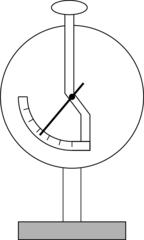
\includegraphics[height=2cm]{Elektrometer}
%\caption{Elektrometer}
%\end{wrapfigure}

Elektrometer: Messung von Ladung ohne Vorzeichen. Beobachtung: 2 Ladungsvorzeichen, Ladungen sind Additiv

\begin{flushleft}
\begin{tabular}{|p{8cm}|}
\hline
\underline{Erhaltungssatz der Ladungen:} In einem geschlossenen System ist die Summe der Ladungen konstant.\\
\hline
\end{tabular}
\end{flushleft}

Erinnerung: geschlossenes System $\widehat{=}$ kein Austausch von Materie mit Umgebung (Ladung gekoppelt an Materie)\\[20pt]
{\large \underline{Noether - Theorem}}\\
Erhaltungssatz $\Leftrightarrow$ Symmetrie des Systems/ Gesetzes.
hier: Eichsymmetrie $U(1)_{Q}\Leftrightarrow$ Ladungserhaltung
(später fortgeschrittene Quantenmechanik, Teilchenphysik)

\subsection{Die Elementarladung}
\textbf{Faraday Elektrolyseexperimente}\\
Bei der Umsetzung von einem Mol eines Elements wird eine feste Ladung umgesetzt.\\
1 wertig: $96486\ \tx{C}/\tx{mol}$ (Faraday Konstante)\\
Also bei der Reaktion eines Moleküls wird $Q=1,6\cdot 10^{-19} \tx{C}$ (Annahme Avogardozahl bekannt, erste Bestimmung 1865 Loschschmidt)\\
\textbf{Frage:} Mittelwert über viele Reaktionen oder fester Wert für jede Reaktion.
\subsection*{Exp: $\rightarrow$ 1913 Millikan - Experiment}
%milikan bild
Kräfte:\\
Gewichtskraft: $$\vec{F}=m\cdot \vec{g}=(\frac{4}{3}\pi r_{\textrm{tröpf}}^3)\rho_{\textrm{Öl}}\vec{g} \downarrow$$
Elektrische Kraft: $$\vec{F_{el}}=Q_{\textrm{tröpf}}\vec{E}\downarrow \uparrow$$
Auftrieb: $$\vec{F_A}=-\frac{4}{3}\pi T^3_{\textrm{tröpf}} \rho_{\tx{Luft}} \vec{g} \uparrow$$
Reibungskraft: $$\vec{F_R}=-G \pi \eta_{\tx{Luft}} \vec{v}_{\textrm{tröpf}} \uparrow \downarrow $$
Laminare Strömung\\
Da $r_{\textrm{tröpf}} \sim \lambda_{\tx{frei}} $\\
$\rightarrow $ Conningham - Korrektur
$$F_R = 1+\frac{\lambda_{\tx{frei}}}{r_{\tx{tropf}}} \bigg(A_1 +A_2 e^{-A_3} \frac{r_{\tx{tropf}}}{\lambda_{\tx{frei}}}\bigg)$$
Luft: $A_1 = 1,257 A_2=0,4 A_3 = 1,1$
\begin{itemize}
\item Suche Tröpfchen
\item Beobachtete Bewegung bei 2. Spannung
\item Bestimme Sink- bzw. Steiggeschwingigkeit
\item $\rightarrow r_{\textrm{tröpf}}$ und $ Q_{\textrm{tröpf}}$
\end{itemize}

\begin{itemize}
\item[a)] Suchmethode
\begin{itemize}
\item sinken bei $0V= U$
\item Erhöhung von U bis Schwebung der Tropfen $\vec{v}_{\textrm{tropf}} = \vec{0}$
\end{itemize}
\item[b)] Steig-/Sink Methode
\begin{itemize}
\item zwei Spannungen $U_c(>0)$ Messe $\vec{r}_{\tx{tropf}}$
\end{itemize}
\end{itemize}
\textbf{Mathode a)} (ohne Conningham Korrektur)\\
$$U = 0V \quad \vert \vec{F}_G \vert = \vert \vec{F}_A \vert + \vert \vec{F}_R \vert$$ (Stationärer Zustand ($\vec{a} = \tx{const}$))
$$\frac{4}{3} \pi \rho_{\tx{Oel}} r^3_{\tx{tropf}} g = \frac{4}{3} \pi \rho_{Luft} r_{\tx{tropf}}^3 g + 6 \pi \eta_{\tx{Luft}} + r \vert \vec{v} \vert$$
$$\Rightarrow r_{\tx{tropf}} = \sqrt{\frac{9}{2g} \frac{\eta_{\tx{Luft}} + \vert \vec{r} \vert }{\rho_{\tx{Oel}}-\rho_{\tx{Luft}}}}$$
Bei Schwebung:
$$U = 0V \quad \vert \vec{F}_G \vert = \vert \vec{F}_A \vert + \vert \vec{F}_{el} \vert$$
$$\frac{4}{3} \pi r^3 \rho_{\tx{Oel}} g = \frac{4}{3} \pi r^3_{\pi} \rho_{\tx{Luft}} + Q_{\tx{tropf}} \frac{U}{d}$$
 d = Abstand Kondensatorplatten
$$Q\pi = \frac{4}{3}	\pi g  \bigg( \rho_{\tx{Oel}}-\rho_{\tx{Luft}} \frac{d}{U}\bigg)$$
viele Tröpfchen $\rightarrow$ Statische Auswertung\\
Ergebnis von Millikan \\%+-unicode
Elektrische Ladung ist gequantelt $+- e;+-2e;\dots$
$$e = 1.6021766208(88) \cdot 10^{-19} C$$
Erstmals gequantelte Größe\\
Drittelzahlige Ladungen der Quarks\\
Quarks sind Konstituenten von Protonen und Neutronen\\
\underline{Proton $p \widehat{=}$ (uud) Neutron $n \widehat{=} $ (udd)}
$$Q_u = + \frac{2}{3}, Q_d = - \frac{1}{3} \Rightarrow Q_p = 1 Q_n = 0$$
$$Q_p + Q_e < 10{-21} e$$ aus Stabilität der Materie\\
\textbf{Historisch:}\\
$Q = 4,774 +- 0,009 \cdot 10^{-10}$esu (Elactrostatic unit)\\
1 esu$ = 3,34 \cdot 10^{-10} C$\\
Millikans wert für Elementarladung: $$ \textrm{esu} \Rightarrow \textrm{SI}: e = 1,592 +- 0,003 \cdot 10 ^{-19} C$$
,,5$\sigma$`` - Effekt $\rightarrow$ Fehler unterschätzt.
\section{Kraft und Feld}
\subsection{Coulomb - Gesetz}
Elektrische Kraft zwischen zwei Körpern (punktförmig) mit Ladungen $Q_1$ und $Q_2$ im Abstand r
$$\vec{F}_{el} = k \frac{Q_1 Q_2}{r^2} , \hspace{0.5cm}\hat{r}_{12} = \frac{\vec{r}_{12}}{\vert\vec{r}_{12} \vert }$$
Kraft auf $Q_2$ von $Q_1$ 
\subsubsection*{Exp: Coulomb - Waage}
$k = 8,99 \cdot 10^{9} \frac{\tx{N m}^2}{C^2}$\\
für $Q_1 = Q_2  =1\tx{ C}$, $r =1\tx { m} \Rightarrow \vert \vec{F}_{el} \vert\  8,99 \cdot 10^{9} \tx{ N}$\
Im SI-System: $k = \frac{1}{4 \pi \epsilon_0}$\\
$\epsilon_0$Dielektrizitätskonstante: $\epsilon_0 = 8,85 \cdot 10^{12} \frac{e^2}{\tx{Nm}^2}$\\
(cgs-System k = 1 $\Rightarrow$ Umdefinition der Ladung)
$$\vec{F}_{el} = \frac{1}{4 \pi \epsilon_0 } \frac{Q_1 Q_2}{r^2}\hat{r}_{12}$$ Coulomb - Gesetz\\
Motivation der Abhängigkeit:
\begin{itemize}
\item $\sim Q_2$ Additivität der Ladungen
\item $\sim Q_1$ ,,actio = reactio``
\item $\sim \frac{1}{r^2}$ dreidimensionaler (für 4 Raumdimensionen wäre es $\sim \frac{1}{r^3}$ )
\end{itemize}

\subsection{Influez}
Beobachtung: Ausschlag des Elektrometers ohne Berührung. Anhängig von der nähe des Stabes.\\
Erklärung: Kraft von $e^-$ auf dem Stab verdrängen die $e^-$ aus der Kugel in die Zeiger.\\
$\Rightarrow$ Kugel positiv geladen, Zeiger negativ geladen\\[5pt]
\underline{Influenz:} Trennung von Ladungen in einem neutralen Körper.\\[5pt]
\underline{In Metallen und Leitern} sind die Elektronen (zu einem bestimmten vom Material abhängigen Grad) frei beweglich.\\
$Q_1 = Q_2$ da neutral
$$\vert \vec{F}_1 \vert = k \frac{Q_1 Q}{r_1^2} \quad \vert \vec{F}_2 \vert = k \frac{Q_2 Q}{r_2^2}\quad  \tx{ da } r_1 < r_2 \quad \vert \vec{F}_1 \vert > \vert \vec{F}_2 \vert$$ Leiter angezogen\\[5pt]
\underline{Nichtleiter:} \\
Ladungen/Elektronen nicht Frei beweglich Verschiebung bei Polaren Molekülen. Wasser $H_2 O$ $\alpha = 105$ $e^-$ vom H zum O verschoben $\rightarrow$ Dipol\\

%Vorlesung 3

\subsection{Das Elektrische Feld}
Bisher: Kraft zwischen zwei Ladungen $ q\textrm{ und } Q \rightarrow \vec{F}$\\
Frage : woher kennt $q$ die Existenz von $Q$ ?\\
$\rightarrow$ abstraktes Konzept: elektrisches Feld $\vec{E}$
\begin{itemize}
\item um jede Ladung $Q$ bildet sich ein Feld $\vec{E}$
\item Probeladung $q$ spürt eine Kraft $ \vec{F} = q \vec{E}$
\end{itemize}
Quantenelktrodynamik (QED): 
\begin{itemize}
\item Anregung des Feldes = Photonen $\gamma $ 
\item Kraft/Wechselwirkung = Austausch von $\gamma$
\end{itemize} 
Pragmatisch: gegben: beliebige Ladungsverteilung wie sieht die Kraft auf eine pkt.förmige $q$ ? ($q \textrm{ klein} \rightarrow \textrm{ keine Verzerrung von } \vec{E})$
$$\rightarrow \vec{E} = \frac{\vec{F}}{q_{\tx{Probe}}} \quad \textrm{ unabhängig von } q_{\tx{Probe}}$$
El. Feld einer Pktladung 
$$ \vec{E} = \frac{\vec{F}_{\tx{Punkt}}}{q_{\tx{Probe}}} = \frac{1}{4 \pi \epsilon_{0}} \frac{Q q_{\tx{Probe}}}{r^2 q_{\tx{Probe}}} \hat{r} = \frac{1}{4 \pi \epsilon_{0}} \frac{Q}{r^2} \hat{r}$$
Zusammenfassung: 
\begin{itemize}
\item jede Ladung $Q$ von $\vec{E}$-Feld umgeben
\item es gilt Superpositonsprinzip $\vec{E}_{Q_1 + Q_2} = \vec{E}_{Q_1} + \vec{E}_{Q_2}$ folgt aus Addition von Kräften
\item Nahwirkung der Kraft: Feld breitet sich mit Lichtgeschwindigkeit $c$ aus
\end{itemize}
Superposition:
\begin{itemize}
\item N Punktladungen $Q_i, i = 1, \dots , N
\qquad \vec{F} = \sum _{i=1}^{N} \vec{F}_i = \frac{1}{4 \pi \epsilon_{0}} \sum _{i=1}^{N} \frac{Q_i}{r^2_i} \hat{r}_i$
$$ \Rightarrow \vec{E} = \sum _{i=1}^{N} \vec{E}_i = \frac{1}{4 \pi \epsilon_{0}}  \sum _{i=1}^{N} \frac{Q_i}{r^2_i} \hat{r}_i$$
\item kontinuierliche \textbf{Ladungsverteilung:} $\rho(\vec{r})$\\[5pt]
Gesamtladung $Q = \int dV \rho(\vec{r'}) \quad (dV = d \vec{r'}^{3})$
$$\vec{E} (\vec{r}) = \frac{1}{4 \pi \epsilon_0} \int d^3 \vec{r'} \frac{\rho (\vec{r'})}{\vert \vec{r}-\vec{r'} \vert ^2} \frac{\vec{r}-\vec{r'}}{\vert \vec{r}-\vec{r'} \vert}$$
\end{itemize}
Visualisierung:
\begin{itemize}
\item[a)] Feldvektoren an vorgegebenen Gitterpunkten im Raume oft Vektor $\widehat{=}$ Projektion von $\vec{E}$ in Ebene
\item[b)] Feldlinien: 
\begin{itemize}
\item Tangenten $\widehat{=}$ Richtung von $\vec{E}$
\item Dichte der Linie $\widehat{=}$ Stärke $\vert \vec{E} \vert$
\end{itemize}
\end{itemize}

\subsubsection*{Exp: Feldlinien} % error blitz orthogonal
\begin{itemize}
\item Feldlinien kreuzen sich nicht [Falls Kreuzung: dann 2 Felder $\vec{E}$ , 2 $\vec{E}$ in einem Punkt wid: Superpositionsprinzip ]
\item Feldlinien $\perp$ orthogonal auf Oberfläche der Leiter
\item keine Feldlinien innerhalb geschlossener Leiter
\end{itemize}
Elektrisches Feld im Leiter
\begin{itemize}
\item $e^-$ frei beweglich und sie stoßen sich ab
\item „Kräftegleichgewicht“ wenn $e^-$ an der Oberfläche sitzen
\item $\vec{E}, \vec{F} \perp$ Oberfläche
\item $\vec{E}$-Feld im Inneren verschwindet
\end{itemize}
Kugel mit Radius: $$ \vec{E}(\vec{R}) = 0 \qquad \vert \vec{r} \vert < R$$
$$ \vec{E}(\vec{r}) = \frac{1}{4 \pi\epsilon_0} \frac{Q}{r^2} \hat{r} \qquad \vert \vec{r} \vert \ge R$$
verhält sich bei großem Abstand wie Punkt-förmige Ladung im Zentrum\\\\
\textbf{Beliebige Flächen:}\\
Approximation durch Ebenen und Kugelschalen
Kugel:
$$ \vert \vec{E} \vert \sim \frac{1}{r^2} $$
kleiner Krümmungsradius $\rightarrow$ großes $ | \vec{E} | $\\
,,Spitze`` $\rightarrow$ kleines r $\rightarrow$ großes $\vert \vec{E} \vert \rightarrow$ führt zur Entladungen\\\\
\textbf{Faradaysche Becher:}
\begin{itemize}
\item begränzte Ladungsaufnahme von außen
\item[$\rightarrow$] Ladungen von innen aufbringen
\end{itemize}
\textbf{Feldberechnung:}
\begin{itemize}
\item[1)] \textbf{homogen geladener Ring} Radius R, Dicke vernachlässigbar
\begin{itemize}
\item $\lambda = \frac{Q}{2\pi R} \qquad [\lambda] = \frac{C}{m}$ Linienladungsdichte
\item gesucht: $\vec{E}(a)$ auf Symmetrieachse (y=z=0)
\item Symmetrie: $\vec{E}(a) = E \vec{e}_x$ [andere Komponenten kompensieren sich]
\item Element auf Ring trägt Ladung $\lambda dx$, liefert Feldbeitrag $$dE_x = \frac{1}{4\pi \epsilon_0} \frac{1}{r^2} \cos \phi dQ$$
\item Es gilt: $$E_x = \cos \phi \vert \vec{E} \vert \qquad \cos\phi = \frac{a}{r} \qquad r= \sqrt{R^2+a^2}$$
\item Integration über Ring in Polarkoordinaten 
\begin{align*}
E_x & = \int_{\tx{Ring}} dQ \frac{1}{4\pi\epsilon_0} \frac{1}{r^2} \cos \phi \\
& = \int_{\tx{Ring}}dQ 
\end{align*}
$$\int_{\tx{Ring}} dQ \frac{1}{4\pi\epsilon_0} \frac{1}{R^2+a^2}\frac{a}{\sqrt{R^2+a^2}} = \frac{Q}{4\pi\epsilon_0} \frac{a}{(R^2+a^2)^{(\frac{3}{2})}}$$
\begin{align*}
\textrm{große Entfernung: }  a\gg R &: & E_x \sim \frac{1}{a^2} \textrm{ wie Pkt.ladung}\\
\textrm{Nähe des Rings: }  a \sim R  &: & \textrm{langsamer Anstieg von }\\ & & \vert \vec{E} \vert \textrm{ als für Pkt.ladung}\\
 a=0&: &E_x = 0  \textrm{ aus Symmetrie }
\end{align*}
\end{itemize}
\item[2)] \textbf{unendlich dünne, unendlich ausgedehnte leitende Platte}\\ Flächenladungsdichte $\sigma \quad [\sigma] = \frac{C}{m^2}$
\begin{itemize}
\item Symmetrie: $\vec{E} = \vec{E}_z \vec{e}_z \perp $ auf Platte
$$Q = \frac{1}{4 \pi \epsilon_0} \int_{V Platte} d^3 \vec{r}\; \rho ( \vec{r})$$

\begin{align*}
\vec{E}(\vec{r}) &= \frac{1}{4 \pi \epsilon_0} \int_{V Platte} d^3 \vec{r}\; \frac{\rho ( \vec{r})}{r^2} \hat{r}\qquad \hat{r} \perp Platte\\
&= \frac{1}{4\pi\epsilon_0} \int_{A Platte} d^2 \vec{r} \; \frac{\sigma}{r^2} \hat{r}
\end{align*}

\item Es gilt: $E_z = \cos\beta \vert \vec{E} \vert \qquad \cos\beta = \frac{a}{d}$\\
Integration in kleinen Ringen bzw. Polarkoordinaten
$(dA = r \; dr \; d\varphi)$
\begin{align*}
E_z(a) &= \frac{1}{4\pi\epsilon_0} \int_0^\infty dr \int_0^{2\pi} d\varphi \; r \frac{\sigma}{a^2} \cos \beta\\[15pt]
&= \frac{\sigma}{4 \pi \epsilon_0a^2} \int_0^\infty dr \int_0^{2\pi} d\varphi \cos^3\beta
\end{align*}
mit $$ r=a\tan \beta\qquad dr = \frac{a}{\cos^2 \beta} d\beta $$
\begin{align*}
r=0 &\ \widehat{ = }\ \beta = 0\\
r=\infty &\ \widehat{ = }\ \beta = \frac{\pi}{2}
\end{align*}
\begin{align*}
E_z(a) &=  \frac{\sigma}{4 \pi \epsilon_0a^2} \int_0^{2\pi} d\varphi \int_0^{\frac{\pi}{2}} a^2 \sin\beta \; d\beta\\
&= \frac{\sigma}{2\epsilon_0} (-\cos\beta) \bigg|_{0}^{\frac{\pi}{2}}\\
&= \frac{\sigma}{2\epsilon_0}
\end{align*}
\item homogenes Feld in z-Richtung (d.h. senkrecht $\perp$ zur Platte)
\end{itemize}
\end{itemize}

%Vorlesung 4

\subsection{Das elektrische Potential}
\begin{itemize}
\item \textbf{Bewegung von Ladung im elektrischen Feld}
$$ W = -\int\limits_{Weg} \vec{F} \; d\vec{s} = -q \int\limits_{Weg} \vec{E} \;d\vec{s}$$
$ W>0:$ von außen gegen $\vec{E}$-Feld verrichten\\
$ W<0:$ Feld verrichtet Arbeit
Charakteristik der Feldes: Arbeit pro Einheitsladung
$$\frac{W}{q} = -\int\limits_{Weg} \vec{E}\;d\vec{s}$$
\item \textbf{Arbeit im Feld einer Punktladung}
$ \vec{E} \perp d\vec{s}$ keinen Beitrag
$$ \frac{W_{ACB}}{q} = -\int_{A}^C |\vec{E}| ds = -\dfrac{1}{a\pi\epsilon_0} \int_{r_A}^{r_C} \frac{Q}{r^2} dr =  -\dfrac{1}{a\pi\epsilon_0} (-\frac{Q}{r}) \mathop{\bigg|}_{r_A}^{r_C} =  -\dfrac{Q}{a\pi\epsilon_0} ( \frac{1}{r_A} - \frac{1}{r_C})$$
analog:
$$\frac{W_{ADB}}{q} = -\int_D^B |\vec{E}| ds =  -\dfrac{Q}{a\pi\epsilon_0} ( \frac{1}{r_D} - \frac{1}{r_B})$$
$$r_A = r_D \quad r_B = r_C \Rightarrow \frac{W}{q} \textrm{ auf beiden Wegen gleich}$$
$$\Rightarrow \oint_{\textrm{geschlossenem Weg}} \vec{E}\; d\vec{s} = 0 \qquad \qquad W \textrm{ unabh. von Weg}$$
+ Superpositionsprinzip $\Rightarrow$ Arbeit auf einem geschlossenen Weg verschwindet (i.e = 0)\\
Erlaubt Definition der potentiellen Energie
$$ E_{pot} (\vec{r}) = -\int_{\vec{r}_0}^{\vec{r}} \vec{E} \; d\vec{s} $$
$\vec{r}_0$ ist ein Bezugspunkt (Referenzpunkt) oft im unendlichen da ($\vec{E}( |\vec{r}| \rightarrow \infty) \rightarrow 0$)
In Praxis: nur
$$ \Delta E_{pot} = E_{pot}(\vec{r}_2) - E_{pot}(\vec{r}_1)$$
relevant.
Normierung von $E_{pot}$ auf im Feld bewegte Ladung:
el. Potential 
$$\varphi(\vec{r}) - \varphi (\vec{r}_0) = \int \vec{E} \; d \vec{s} \qquad \qquad \textrm{ oft } \varphi(\vec{r}_0) = 0$$
$$\varphi(\vec{r}) = \int \vec{E} \; d \vec{s}$$
Für Punktladung Q $\quad \vec{r}_0 \rightarrow \infty :$ $$\varphi(\vec{r}) = \frac{1}{4\pi\epsilon_0} \frac{Q}{|\vec{r}|}$$
\item \textbf{Superpositionsprinzip:}\\
N Punktladungen $Q_i$ bei $\vec{r}_i$
$$ \varphi(\vec{r}) = \sum_{i=1}^N \varphi_i(\vec{r}) = \sum_{i=1}^N \frac{1}{4\pi\epsilon_0} \frac{Q_i}{|\vec{r}-\vec{r}_i|}$$
\textbf{Potential ist Skalarfeld} $\rightarrow$ Rechnungen oft einfacher, graphische Darstellung mittels Äquipotentialflächen: \\
(auf diesen gilt $\varphi(\vec{r}) = \const$)
\begin{itemize}
\item für Pkt. Ladung: Äquipotentialflächen = Kugelschalen
\item Feldlinien / $\vec{E}$-Feld $\perp$ Äquipotentialflächen
\item Bewegung in Äquipotentialflächen $\rightarrow$ keine Arbeit wird verrichtet
\end{itemize}
\textbf{Zusammenhang elektrisches Feld $\vec{E}$ und Potential $\varphi$}\\
Wir hatten: $$\varphi(\vec{r}) = - \int_{\vec{r}_0}^{\vec{r}} \vec{E} \; d \vec{s} \qquad \varphi(\vec{r}_0) = 0$$
Ist dies umkehrbar?
\begin{itemize}
\item[a)] infinitesimaler Weg $dx$, Probeladung $q$
\begin{align*}
dW &= -q [ \varphi(x,y,z) - \varphi(x + dx,y,z] \\[10pt]
&= q \frac{\varphi(x+dx,y,z) - \varphi(x,y,z)}{dx} dx \\[10pt]
& = q \frac{\partial \varphi(x,y,z)}{\partial x} dx
\end{align*}
\item[b)]
\begin{align*}
dW &= -q \vec{E}(\vec{r}) \; d\vec{s} \qquad d\vec{s} = \begin{pmatrix}
dx\\
0\\
0\\
\end{pmatrix}\\
&= -q E_x\;dx
\end{align*}
Vgl: $$E_x = -\frac{\partial \varphi}{dx}$$
analog zu Bewegung in y- und in z-Richtung
\begin{align*}
\vec{E} (\vec{r}) &=  \bigg( - \frac{\partial \varphi}{\partial x} \vec{e}_x \bigg) + \bigg( - \frac{\partial \varphi}{\partial y} \vec{e}_y \bigg) + \bigg( - \frac{\partial \varphi}{\partial z} \vec{e}_z \bigg)\\[10pt]
&= -\textrm{grad}\; \varphi(\vec{r}) = - \vec{\nabla} \varphi(\vec{r}) \qquad \qquad \qquad \vec{\nabla} = \begin{pmatrix}
\frac{\partial \varphi}{\partial x} \\
\frac{\partial \varphi}{\partial y} \\
\frac{\partial \varphi}{\partial z} 
\end{pmatrix}
\end{align*}
\end{itemize} 
Elektrostatik: äquivalente Beschreibung durch entweder $\vec{E}$-Feld oder $\varphi$\\
\end{itemize}
\underline{Wirbelfreiheit von $\vec{E}$}
Rotation von 
\begin{align*}
\vec{E}:\; \tx{rot}(\vec{E}) &= \vec{\nabla} \times \vec{E} \\
&= \bigg( \frac{\partial E_z}{\partial y} - \frac{\partial E_y}{\partial z} \bigg) \vec{e}_x + \bigg( \frac{\partial E_x}{\partial z} - \frac{\partial E_z}{\partial x} \bigg) \vec{e}_y + \bigg( \frac{\partial E_y}{\partial x} - \frac{\partial E_x}{\partial y} \bigg) \vec{e}_z
\end{align*}
da $\vec{E} = \textrm{grad} \varphi $ und 
$$ \frac{\partial^2 \varphi}{\partial y \partial x} = \frac{\partial^2 \varphi}{\partial x \partial y}$$
Partielle Ableitungen vertauschbar
$$ \Rightarrow \quad \textrm{rot} \vec{E} = - \textrm{rot}(\textrm{grad} \varphi ) = \vec{0}$$
$\vec{E}$-Felder in Elektrostatik sind Wirbelfrei\\
Zusammenhang: mit Stokesschem Satz
$$\int\limits_{A} \vec{\nabla} \times \vec{V}(\vec{r}) \; d\vec{A} = \oint\limits _{S= dA} \vec{V}(\vec{r}) \; d \vec{s} \qquad \vec{V}(\vec{r}) \textrm{Vetorfeld}$$
hier
$$\int_{A} \tx{rot}(\vec{E}) \; d\vec{A} = \oint_{\delta A} \vec{E} \; d\vec{s} \buildrel \textrm{\ E. statik}\over= 0 $$
Bedeutung: wirbelfrei bzw. keine geschlossenen Feldlinien\\[5pt]
\textbf{Beispiele Potential-Berechung:}
\begin{itemize}
\item[1)] Potential eines homogenen ringförmigen Leiters. Beitrag $d\varphi$ aus $dQ$ auf Ring
$$ d\varphi = \frac{1}{4\pi\epsilon_0} \frac{1}{r} \;dQ$$
Aus Abbildung: $r = \sqrt{R^2 + a^2}$
$$ \varphi(a) = \frac{Q}{4\pi\epsilon_0} \frac{1}{\sqrt{R^2 + a^2}}$$
da $r = \const$ auf x-Achse\\
für $a\gg R \quad \varphi(a) = \frac{Q}{4\pi\epsilon_0} \frac{1}{a}$ Potential einer Pkt. Ladung
$$E_x = -\frac{\partial \varphi(a)}{\partial a}= -\frac{\partial\varphi(x)}{\partial x} = -\frac{Q}{4\pi\epsilon_0} \frac{1}{(R^2 + a^2)^{\frac{3}{2}}} \left(-\frac{1}{2}\right) 2 a = \frac{1}{4\pi\epsilon_0} \frac{Q a}{(R^2 + a^2)^{\frac{3}{2}}}$$
\item[2)] Beispiel 2: leitende Kugel Radius R
$$\varphi(a) = \frac{Q}{4\pi\epsilon_0} \frac{1}{a} \qquad a\ge R$$
$$ \varphi(a) = \frac{Q}{4\pi\epsilon_0} \frac{1}{R} = \tx{const.} \qquad a < R$$
\begin{align*}
\rightarrow \vec{E} = - \grad \varphi &= \frac{Q}{4\pi\epsilon_0} \frac{1}{a^2} \vec{e}_R \qquad a\ge R \\
 &= 0 \Rightarrow \qquad a < R
\end{align*}
Bisher: $\varphi(\vec{r})$ aus $\rho(\vec{r})$ via Poisson-Integral teilweise $\rho(\vec{r})$ nicht bekannt, aber Randbedingungen $\varphi(\vec{r}) = 0 $ auf Leiteroberfläche. ($\rho(\vec{r})$ kann komlex sein)\\
$\Rightarrow$ Randwertproblem (Theo II.)
\end{itemize}
,,Einfaches`` Beispiel mit \textbf{Methode der \underline{Spiegelladung}}\\
Platte geerdet $\ \varphi(x,y,z) \buildrel ! \over = 0 \ $
Punktladung $q_1$ bei $\ \vec{r} = \begin{pmatrix}
0\\
0\\
z_1
\end{pmatrix}$\\
Realisierung der Randbedingungen durch Spiegelladung $q_2$\\
Brauche: $\varphi(x,y,z=0) = 0$\\
Superposition $\varphi = \varphi_1 + \varphi_2$\\
$\Rightarrow q_2 = - q_1 \quad z_2 = - z_1$ erfüllen Randbedingung\\
$$\varphi(\vec{r}) = \frac{a_r}{4\pi\epsilon} \bigg\{ \frac{1}{|\vec{r}-\vec{r}_1|} - \frac{1}{| \vec{r} - \vec{r}_2|} \bigg \} \quad $$

$\vec{E}$-Feld aus $-\vec{\nabla}^2 \varphi$\\
$$ \vec{E}(\vec{r}) = \frac{a_r}{4\pi\epsilon_0} \bigg\{ \frac{\vec{r} - \vec{r}_1}{|\vec{r} - \vec{r}_1|^3} - \frac{\vec{r} - \vec{r}_2}{|\vec{r} - \vec{r}_2|^3} \bigg\}$$
für z=0 : $ E_x = E_y = 0 \quad \vec{E} \perp (x,y)$-Ebene\\
Flächenladungsdichte: $\sigma \quad [\sigma] = \frac{C}{m^2}$\\
Später: $ \sigma = 2 \epsilon_0 E_z$
$$\sigma = - \frac{q_1}{2\pi} \frac{z_1}{(x^2+y^2+z_1^2)}$$
$$ \vec{r}_1 = \begin{pmatrix}
0\\0\\z_1
\end{pmatrix}$$

\subsection{Der elektrische Fluss}
Elektrischer Fluss $\Phi$ ist ein Maß für die dichte der el. Feldlinien. Er ist definiert für eine gegebene Fläche A.
$$ \boxed{\Phi_A = \int_{A} \vec{E} \;d \vec{A}} \qquad \vec{A} = \textrm{infinitisimaler Normalvektor} \qquad \vec{A} \perp \textrm{ Fläche }$$
offene Fläche: Orientierung beliebig\\
geschlossene Fläche: Orientierung nach außen\\[5pt]
\subsubsection{Fluss durch geschlossene Fläche:}
Bsp: \textbf{Würfel im Plattenkondensator} (Abb.auf \folie{Elektrischer Fluss durch geschlossene Oberfläche}) nur Beiträge von linker und rechter Fläche:
$$
\begin{tikzpicture}[scale=.6]
\draw[thick,draw=black,fill=yellow] (0,0)--(1,1)--(4,1)--(4,-1)--(2,-2)--(0,-2)--(0,0);
\draw[draw=none,fill=black,opacity=.15](2,0)--(4,1)--(4,-1)--(2,-2)--(2,0);
\draw[thick,draw=black](0,0)--(2,0)--(2,-2);
\draw[thick,draw=black] (2,0)--(4,1);
\draw[dashed,thick] (2,0) -- (3,1);
\draw[thick,draw=red] (3,.5) arc (25:55:.7cm);
\node[red] at (3.2,.8) {$ \alpha $};
\node at (0,.5) {$ l $};
\node at (3,.1) {$ l_r $};
\draw (-.5,.1)--(0,.1);
\draw (-1.5,-.4)--(0,-.4);
\draw (-.5,-.8)--(0,-.8);
\draw (-1.5,-1.2)--(0,-1.2);
\draw[->] (3.5,.1)--(4.5,.1);
\draw[->] (2.5,-.4)--(3.5,-.4);
\draw[->] (3.5,-.8)--(4.5,-.8);
\draw[->] (2.5,-1.2)--(3.5,-1.2);
\node at (-2,-.6) {$ \vec{E} $};
\end{tikzpicture}
$$
$$ \Phi = \Phi_l + \Phi_r = \vec{E} \vec{A}_l + \vec{E} \vec{A}_r = -E A_l + E A_r \cos \alpha = -EA_l + E A_l= 0$$
$$ \vec{A}_l = - \vec{A}_r \cos \alpha$$
Superposition bzw. Approximation von Körper durch inf. Würfel $\Rightarrow$ Fluss durch geschlossene Oberfläche im homogenen Feld verschwindet.\\
Bsp: Kugelschale
$$\vec{A}(r) = 4 \pi r^2 \vec{e}_R \left\{\begin{array}{ll}
+ & \textrm{ für äußere} \\
- & \textrm{ für innere}
\end{array}\right.$$
$$\vec{E}(\vec{r}) = \frac{Q}{4\pi\epsilon_0} \frac{1}{r^2} $$
$$\bigg | \vec{E}(\vec{r}) \cdot \vec{A}(\vec{r}) \bigg | = \textrm{ const}$$
$$\Phi = \Phi(r_1) + \Phi(r_2) = + \textrm{ const} - \textrm{ const} = 0$$
In elektrischen Feldern (wenn keine Ladungen im Volumen) $\Rightarrow $ Fluss durch geschlossene Oberfläche verschwindet.

\subsection{Quellstärke des elektrischen Feldes}
$\Phi_A \neq 0$ wenn Ladungen innerhalb geschlossener Oberfläche. Bsp: Kugel mit Radius R. Punktladung im Ursprung $d\vec{A}$ und $\vec{E}$ radial nach außen $\sim \vec{e}_r$ 
$$\Phi = \oint\limits_{\textrm{R = const}} \vec{E}\; d \vec{A} = \underbrace{\frac{1}{4\pi\epsilon_0} \frac{Q}{R^2}}_{|\vec{E}|}\  \underbrace{4\pi R^2}_{A} = \frac{Q}{\epsilon_0}$$
Ergebnis unabhängig von:
\begin{itemize}
\item Form der Oberfläche
\item Position der Ladung innerhalb der Oberfläche
\end{itemize} 
Mehrere Ladungen $Q_i$ aus Superposition der $\vec{E}_i$ 
$$\Phi = \oint \Big(\sum_i \vec{E}_i\Big) \;d \vec{A} = \frac{\sum_i Q_i}{\epsilon_0}$$
,,externe`` $Q_i$ liefern keinen Beitrag\\
Es gilt:
$$\boxed{\Phi = \oint \vec{E}\; d\vec{A} = \frac{Q_{\tx{ein}}}{\epsilon_0}} $$
Gaußsches Gesetz (Integralform)\\
Mit Gaußschen Satz : Oberflächen- $\rightarrow$ Volumenintegral\\
$$ \oint_A \vec{E} \;d \vec{A} = \int_V \textrm{div} \vec{E} \; d \vec{V} \quad \textrm{mit} \quad Q_{\tx{ein}} = \int_V \rho(\vec{r})\;dV$$
$$\int_V \textrm{div} \vec{E}\; dV = \frac{1}{\epsilon_0} \int_V \rho(\vec{R}) \; dV$$
gültig für beliebige Volumen\\
$\Rightarrow \textrm{div} \vec{E}=\frac{\rho}{\epsilon_0}$ differentielle Form des Gaußschen Gesetzes\\
Ladungen die Quellen $(\rho > 0 )$ bzw. Senken $\rho < 0)$ des elektrischen Feldes sind.

\subsection{Maxwell-Gleichungen}
für statische (unbewegte) Ladungen
Integral- und Differentialform \\
\begin{eqnarray*}
\phantom{\qquad \qquad \qquad \qquad \qquad}\boxed{\oint \vec{E}\; d\vec{s} = 0 \quad \tx{rot}\vec{E} = \vec{0}\ \ \textrm{ Wirbelfrei }} \qquad \quad \qquad \quad \ \ (1)\\
\boxed{\oint \vec{E} \; d\vec{A} = \frac{Q_{\tx{ein}}}{\epsilon_0} \quad \tx{div}\vec{E}= \frac{\rho}{\epsilon_0}  \ \ \textrm{ Quellen/Senken}}  \qquad \qquad (3)
\end{eqnarray*}
1. gilt allgemein in Zentralkraftfeldern d.h. $\rho(\vec{r}) \sim |\vec{r}|$\\
3. gilt nur für $\varphi \sim \frac{1}{|\vec{r}|} | \vec{E} | \sim \frac{1}{|\vec{r}|^2}$ im 3-dimensionalen Raum\\[10pt]
MW-Gleichungen sind Axiome der Elektrostatik d.h. $F_{\tx{coulomb}}$ ableitbar\\
betrachte Ladungen $Q_1 = Q_{\tx{ein}}$\\
1.Gl: $$\oint_A \vec{E}\; d\vec{A} = \frac{Q_1}{\epsilon_0}$$
$$|\vec{E}(r)| 4 \pi r^2 = \frac{Q_1}{\epsilon_0}$$
Kraft auf Ladung $Q_2$: $\vec{F}_{Q_2} = \vec{E}_{Q_1} \cdot Q_2$
$$|\vec{F}_{Q_2}| = \frac{Q_1 Q_2}{4\pi\epsilon_0} \frac{1}{r^2}$$ 
\begin{flushright}
$\square$
\end{flushright}
Bsp.: \textbf{homogene geladene Kugel}, Radius R, $\rho(\vec{r}) = \textrm{const}\quad |\vec{r}| \le R$
$$ Q_{\tx{ges}} = \frac{4}{3} \pi R^3 \rho$$
Symmetrie:  $ \vec{E} = |\vec{E}| \vec{e}_r\ $ radial $\  |\vec{E}| = E_r$\\
\begin{itemize}
\item[$|\vec{r}|\ge R$:] $$\Phi = \oint_A \vec{E} \; d \vec{A} = \int_A E_r \; dA = E_r 4 \pi r^2 \buildrel ! \over = \frac{Q_{ein}}{\epsilon_0}$$
$$ E_r = \frac{\rho_0 R^3}{\epsilon_0 3 r^2}$$
wie bei Punktladung
\item[$|\vec{r}|\le R$:] $$ Q_{\tx{ein}} = \frac{4}{3} \pi r^3 \rho \qquad \Phi = \frac{Q_{\tx{ein}}}{\epsilon_0}$$\\
$$ E_r = \frac{\rho_0 r}{3 \epsilon_0}$$ linearen Anstieg
\end{itemize}
\noindent
Potential $\varphi(\vec{r})$:\\
$\varphi(r_0 = \infty) = 0$\\
$$\varphi(r) = -\int_\infty ^r \vec{E}\; d\vec{r} \buildrel (r\ge R) \over = -\int_\infty ^r \frac{\rho R^3}{\epsilon_0 3 r'^2}\; dr' =   \int_{r}^{\infty} \frac{\rho}{\epsilon_0} \frac{R^3}{3 r'^2}\; d r' = \frac{\rho R^3}{\epsilon 3 r}$$
$$\Big(\frac{\partial (\hat{r})}{\partial r} = - \frac{1}{r^2}\Big)$$
Innenraum: $(r\le R)$
$$\varphi (r) = -\int \frac{\rho r'}{3 \epsilon_0 } \; dr' = -\frac{1}{2} \frac{\rho_0}{\epsilon_0} \frac{r^2}{3} + \textrm{const}$$
Wähle c so, dass $\varphi$ stetig bei $r = R$ ist\\
$\rightarrow c = \frac{R^2 \rho}{2 \epsilon_0}$
$$\varphi(r) = \frac{R^2 \rho}{2 \epsilon_0} (1 - \frac{r^2}{3 R^2} ) \quad \textrm{ für } r\le R$$
\textbf{Maxwell-Gl. und Potential $\varphi$}
$$\vec{E} = -\textrm{grad}(\varphi)$$
1. Gl $$\textrm{rot}\vec{E} = - \textrm{rot}(\textrm{grad} \varphi )\buildrel \tx{linear} \over = 0$$
da rot$\vec{E} = 0$ können wir $\vec{E}$ als grad$\varphi$ schreiben\\
3. Gl $$\textrm{div}\vec{E} = \textrm{div}(-\textrm{grad} \varphi) = -\Big[\frac{\partial^2 \varphi}{\partial x^2} + \frac{\partial^2 \varphi}{\partial y^2} + \frac{\partial^2 \varphi}{\partial z^2} \Big] = - \Delta \phi$$
$$\rightarrow \quad -\Delta \phi = \frac{\rho}{\epsilon_0}$$ 
Poisson-Gl. ($\rho = 0$ Laplace-Gl.)\\
Poisson-Gl. äquivalent zu beiden Maxwell-Gl.\\
MW-Gl: 2 Gl. erster Ordnung in Ableitungen $(\frac{\partial}{\partial x} ,\dots )$\\
Poisson-Gl: 1.Gl. zweiter Ordnung in Ableitung $(\frac{\partial^2}{\partial x^2} , \dots )$\\

\section{Multipole}
\begin{itemize}
\item für beliebige Ladungsverteilung $\rho(\vec{r})$ ist $$ \Phi (\vec{r}) = \frac{1}{4\pi\epsilon_0} \int d^3 \vec{r'} \frac{\rho(\vec{r}\: ')}{|\vec{r}-\vec{r}'|}$$ komplex i.a.
\item oft interessiert nur Fernfeld $\rho(\vec{r}), \vec{E}(\vec{r}),\ \ |\vec{r}| \gg | \vec{r'}|\ $ mit $\ \rho(\vec{r'}) = 0$\\
Abstand $\gg$ Ausdehnung der Ladungsverteilung
\item Approximation von $\rho(r)$ in Taylor-Entwicklung\\
$\rightarrow$ Multipolentwicklung
$$\rho(\vec{r}) = \underbrace{\frac{a}{T}}_{\tx{Monopol}} + \underbrace{\frac{b}{T^2}}_{\tx{Dipol}} + \underbrace{\frac{c}{T^3}}_{\tx{Quadropol}} + \dots$$ 
\end{itemize}
\textbf{Monopol:}\\
$$\vec{E}_{\tx{Mono}}(\vec{r}) = \frac{1}{4\pi\epsilon_0} \frac{Q}{r^2} \hat{r} \qquad \varphi_{\tx{Mono}}(\vec{r}) = \frac{Q}{4\pi\epsilon_0} \frac{1}{r}$$
dominiert für $r\rightarrow\infty$ wenn $Q_{\tx{ges}} \neq 0$\\
$$Q_{\tx{Mono}} = \sum_{i=1}^N Q_i \textrm{ Pkt. Ladungen } \quad Q_{\tx{Mono}} = \int d^3\vec{r} \rho (\vec{r})$$
$Q_{\tx{Mono}}$ bei $\vec{r}_s$ Ladungsschwerpunkt platzieren\\
$$\vec{r}_s = \frac{\sum_i |Q_i| \vec{r}_i}{\sum_i | Q_i|}$$
$$\vec{r}_s = \frac{\int|\rho(\vec{r})| \vec{r} d^3 \vec{r}}{\int|\rho(\vec{r})| d^3\vec{r}}$$
\textbf{Dipol:}\\
zwei entgegengesetzte, gleich große Ladungen $Q>0$ im Abstand $d = |\vec{d}|$. Richtung $\vec{d}$ von $-Q$ nach $+Q$ 
$$\vec{r}_- = \vec{r}_0 - \frac{\vec{d}}{2} \qquad \vec{r}_+ = \vec{r}_0 + \frac{\vec{d}}{2}$$
Potential $\varphi(\vec{r})$ aus Superposition
$$\varphi_{\tx{Dipol}} (\vec{r}) = \frac{Q}{4 \pi \epsilon_0} \bigg\{ \frac{1}{|\vec{r}_0 - \frac{\vec{d}}{2}|} - \frac{1}{|\vec{r}_0 - \frac{\vec{d}}{2}|} \bigg\}$$ 
für $(|\vec{r}_0| \gg |\vec{d}|)$ nutze Näherung 
$$\frac{1}{|\vec{r}_0 \pm \frac{\vec{d}}{2}|} = \frac{1}{\sqrt{\vec{r}_0^{\,2} \pm r_0 \vec{d} + \frac{\vec{d}^2}{4}}} = \frac{1}{|\vec{r}_0|} \frac{1}{\sqrt{1 \pm \frac{r_0 \vec{d}}{|\vec{r}_0|^2} + \frac{\vec{d}^{\,2}}{4 \vec{r}_0^{\,2}}}} =  \frac{1}{|\vec{r}_0|} \bigg( 1 \mp \frac{\vec{r}_0 \vec{d}}{\vec{r}_0^{\,2}}\bigg)$$
$$\varphi_{\tx{Dipol}} \sim \frac{Q}{4\pi\epsilon_0 r} \frac{\vec{r}\vec{d}}{r^2} = \frac{1}{4\pi\epsilon_0} \frac{\vec{p}\;\vec{\hat{r}}}{r^2} $$
$ \vec{p} = Q \vec{d} = [\vec{p}] = c_m$ \textbf{Dipolmoment}
$$\varphi_{\tx{Dipol}} (\vec{r}) = \frac{Q\vec{d}}{4\pi\epsilon_0} \frac{\cos \theta}{r^2} \qquad \theta = \sphericalangle (\vec{d}, \vec{r})$$
\begin{itemize}
\item Potential richtungsabhängig $\sim \cos \theta$\\
maximal entlang $\vec{d}$ verschwindend $\perp \vec{d}$
\item $\varphi \sim \frac{1}{r^2} \Rightarrow \ $ Erwartung $|\vec{E}| \sim \frac{1}{r^3}$
\end{itemize}
\textbf{Bestimmung des $\vec{E}$-Feldes:}\\
$\vec{d}$ entlang z-Achse\\
Geometrie $\rightarrow$ Zylindersymmetrie des Feldes, d.h. keine Abhängigkeit vom Azimutalwinkel $\phi$ 
$$\vec{E}(\vec{r}) = - \vec{\nabla} \varphi(\vec{r}) = -\frac{\partial \varphi}{\partial r} \vec{e}_r - \frac{1}{r} \frac{\partial \varphi}{\partial \theta} \vec{e}_\theta = \frac{1}{r \sin \theta} \underbrace{\frac{\partial \varphi}{\partial \phi}}_{\varnothing} \vec{e}_\varphi$$
$$ \vec{E} (\vec{r}) = \frac{1}{4\pi\epsilon_0 r^3} \; |\vec{p}| \; (2 \cos \theta \vec{e}_r + \sin \theta \vec{e}_\theta ) $$
\begin{itemize}
\item für N Punktladungen $\vec{p} = \sum_i Q_i \vec{r}_i$
\item für Ladungsverteilung $\vec{p} = \int d^3 \vec{r} \ \rho (\vec{r}) \vec{r} $
\end{itemize}
$\vec{p}$ abhängig von Wahl des Koordinatenursprungs\\[10pt]
Bsp.: Punktladung bei $\vec{r}_0 \Rightarrow \left\{ \begin{array}{cccc}
\textrm{i)} & \vec{r}_0 = \vec{0} & \textrm{dann} & \vec{p} = \vec{0} \\
\textrm{ii)} & \vec{r}_0 \neq \vec{0} & \textrm{dann} & \vec{p} \neq \vec{0}
\end{array} \right. $ \\[10pt]
Konvention: Ursprung bei $\vec{r}_s$ Ladungsschwerpunkt
\begin{itemize}
\item punktsymmetrische Ladungsverteilung $ \rho(\vec{r}) = \rho(-\vec{r})$ gilt $\vec{p} = \vec{0}$
\item wenn $Q_{\tx{ges}} = 0$ dann $\vec{p}$ unabhängig von Ursprung
\end{itemize}

%Vorlesung 5 oder so

\subsection{Kräfte auf Dipol}
\begin{itemize}
\item[a)] \textbf{homogenes $\vec{E}$-Feld} (Bsp. Plattenkondensator)\\
Beobachtung: Dipol richtet sich im Kondensator wie erwartet aus: Plus zu Minus, Minus zu Plus\\
Kraft: $$\vec{F}_{ges} = Q \vec{E} + (-Q) \vec{E} = \vec{0}$$ $\rightarrow$ keine Translation\\
Drehmoment: \begin{align*}
\vec{T}_{ges} & = \sum^2_{i=1} \vec{r}_i\times \vec{F}_i \\
& = \frac{\vec{d}}{2} \times Q\vec{E} + \frac{-\vec{d}}{2} \times (-Q\vec{E}) = Q \vec{d} \times \vec{E}\\
\end{align*}
$$\boxed{\vec{T}_{ges} = \vec{p} \times \vec{E}}$$
$\vec{p} \perp \vec{E} \quad \vec{T}$ Maximal\\
$ \vec{p} \parallel \vec{E} \quad \vec{T}$ verschwindet\\
$\rightarrow$ Ausrichtung im $\vec{E}$-Feld\\
Potentiellen Energie:\\
$$ E_{\tx{Dip}}= Q \varphi(\vec{r}_1) - Q \varphi(\vec{r}_2)$$
$$\varphi(\vec{r}_1) - \varphi(\vec{r}_2) = \vec{\nabla} \varphi(\vec{r}) \vec{d} = -\vec{E} \vec{d}$$
$$E_{\tx{Dip}} = - Q \vec{E}\vec{d} = - \vec{p} \vec{E}$$\\
$p \uparrow \uparrow E$ minimiert $E_{Dip} \quad \rightarrow$ Richtung von $\vec{p}$ im $\vec{E}$
\item[b)] \textbf{inhomogenes $\vec{E}$-Feld} \\
zusätzliche Kraft: $$\vec{F}_{ges} = Q \vec{E} (\vec{r}+\vec{d}) - Q \vec{E}(\vec{r})$$
$$\vec{E}(\vec{r}+\vec{d}) \buildrel \textrm{Taylor-Entwicklung} \over = \vec{E}(\vec{r}) + (\vec{d}\cdot \nabla ) \vec{E}(\vec{r})$$ 
$$\vec{F}_{ges} = Q ( \vec{q} \cdot \nabla ) \vec{E}(\vec{r}) = (\vec{p} \cdot \nabla ) \vec{E}(\vec{r})$$
\begin{itemize}
\item[i)] Ausrichtung von Dipol durch $\vec{T}_{ges}$
\item[ii)] Bewegung ins Gebiet höherer Feldstärke $\vec{E}$
\end{itemize}
\end{itemize}

\subsection{Quadrupol}
\begin{itemize}
\item vier Ladungen $ 2: \; +Q$, $ 2: \; -Q$ , jeweils im Abstand $d$
\item zwei Dipole $\vec{p}$ bei $(x,z) = (\frac{d}{2}, 0) \quad -\vec{p}$ bei $(x,z) = (-\frac{d}{2}, 0)$
$$ \varphi_{\tx{Dipol}} = \frac{1}{4\pi\epsilon_0} \frac{\vec{p}\vec{r}}{r^3} = \frac{1}{4\pi\epsilon_0} \frac{p \cos \theta}{r^2} \qquad \vec{r}_s = \vec{0} \quad \theta = \sphericalangle (\vec{r}, \vec{e}_z)$$
$$\varphi _{\tx{Quadrupol}} = \varphi_{\tx{oben}}(\vec{r}- \frac{\vec{d}}{2}) - \varphi_{\tx{unten}}(\vec{r}+ \frac{\vec{d}}{2})$$
für $|\vec{d}|$ klein : $$\approx -d \frac{\partial}{\partial x } \varphi_{\tx{Dipol}} (\vec{r})$$
$$\frac{\partial }{\partial x} \varphi_{\tx{Dipol}} = \frac{1}{4\pi\epsilon_0} \bigg[ -2 \frac{p \cos \theta}{r^3} \frac{\partial r }{\partial x} - \frac{p \sin \theta }{r^2} \frac{\partial \theta}{\partial x} \bigg]$$
\end{itemize}
Kettenregel: 
$$ \frac{\partial}{\partial x} = \frac{\partial r}{\partial x} \frac{\partial}{\partial r} \quad \frac{\partial}{\partial x} = \frac{\partial \theta}{\partial x} \frac{\partial}{\partial \theta}$$
Kugelkoordinaten: $$ \begin{pmatrix}
x\\
y\\
z
\end{pmatrix} = \begin{pmatrix}
r \sin \theta \cos \phi \\
r \sin \theta \sin \phi \\
r \cos \phi
\end{pmatrix}$$
$$ \frac{\partial r}{\partial x} = \frac{\partial}{\partial x} \sqrt{x^2+y^2+z^2} = \frac{1}{r^2} 2x = \frac{x}{r} = \sin \theta \cos \phi $$
$$\frac{\partial \cos \theta}{\partial x} = -\frac{1}{r} \sin \theta \sin \phi \cos \phi$$
\begin{align*}
\varphi_{\tx{Quadrupol}}(\vec{r}) &= -\frac{|\vec{p}||\vec{d}|}{4\pi\epsilon_0} \bigg\{ - \frac{2 \cos \theta }{r^3} \sin \theta \cos \phi - \frac{\sin \theta}{r^2} \frac{1}{r} \cos \theta \cos \phi \bigg\} \\
& = \  \frac{3|\vec{p}||\vec{d}|}{4\pi\epsilon_0 r^3} \cos \theta \sin \theta \cos \phi
\end{align*}
$$Q_{\tx{Mono}} = 0  \quad \vec{p}_{\tx{gesamt}} = \vec{0}$$
Fernferld: $$ \varphi(\vec{r}) \sim \frac{1}{r^3} \quad \textrm{bzw.} \quad \vec{E} (\vec{r}) \sim \frac{1}{r^4} \vec{e}_R$$
Bsp.: linearer Quadrupol
$$\varphi^{\tx{lin}}_{\tx{Quad}} = \frac{1}{4\pi\epsilon_0} \frac{|\vec{a}|^2Q}{r^3} (3 \cos^2\theta -1)$$
\subsubsection{Kraft und Elektrische Energie des Quadrupols}
\begin{itemize}
\item homogenes Feld: $\vec{F}_{\tx{ges}} = \vec{0} \quad ; \quad \vec{T}_{\tx{ges}} = \vec{0}$
\item inhomogenes Feld : komplexe $\vec{F}_{\tx{ges}}$ , $\vec{T}_{\tx{ges}}$
\end{itemize}
Elektrische Energie
$$ E_{el} = \sum ^4_{i=1} Q_i \varphi_{\tx{ext}}(\vec{r}_i) \quad \textrm{(eine kleine Rechnung)}$$
$$ E_{el} = Q |\vec{d}|^2 \frac{\partial ^2 \varphi_{\tx{ext}}}{\partial x \partial y} = \frac{1}{3} \hat{Q}_{xy} \frac{\partial ^2 \varphi_{\tx{ext}}}{\partial x \partial y} $$
$$\hat{Q}_{x_1} = 3 Q |\vec{d}|^2 \textrm{ Quadrupol}$$
allgemein gilt : 
für $ x_1 \widehat{=} x, x_2 \widehat{=} y, x_3 \widehat{=} z$
$$E_{el} = \frac{1}{6} \sum^3_{i,j=1} \hat{Q}_{ij} \frac{\partial ^2 \varphi_{ext}}{\partial x_i \partial x_j}$$
$$\hat{Q}_{ij} = \int d^3 \vec{r} \{ 3x_ix_j - |\vec{r}|^2 \delta_{ij} \} \rho (\vec{r})$$
Tensor 2. Stufe $i,j = 1 \rightarrow 3$\\
für N Punktladungen : $$\hat{Q}_{ij} = \sum^N_{k=1} (3x_ix_j)_n - |\vec{r}|^2 \delta_{ij} \qquad \delta_{ij}= \casess{i=j}{1}{i \neq j}{\tx{sonst}} = \begin{pmatrix}
1 & \cdots & 0 \\
\vdots & \ddots & \vdots\\
0 & \cdots & 1 
\end{pmatrix}$$

$E_{el}$ in Multipolentwicklung

\begin{align*}
E_{el} &= Q_{\tx{ges}} \varphi_{\tx{ext}} (\vec{r})  + \sum^3_{i=1} p_i \frac{\partial \varphi_{\tx{ext}}}{\partial x_i} + \frac{1}{6} \sum^3_{i,j = 1} \hat{Q}_{ij} \frac{\partial ^2 \varphi_{\tx{ext}}}{\partial x_i \partial x_j} \\
&= Q_{\tx{Mono}} \varphi_{\tx{ext}}(\vec{r}) + \underbrace{\vec{p} \; \vec{\nabla} \varphi_{\tx{ext}} (\vec{r})}_{\tx{Dipolanteil}} + \underbrace{ \frac{1}{6} \sum^3_{i,j = 1} \hat{Q}_{ij} \frac{\partial ^2 \varphi_{\tx{ext}}}{\partial x_i \partial x_j} }_{\tx{Quadrupolanteil}}
\end{align*}
Bem.: $\vec{p}, \hat{Q}$ abhängig von Wahl des Koordinatensystems
\section{Elektrostatische Energie und Kapazität}
\subsection{Spannung}
Erinnerung: $$\varphi(\vec{r}) = \frac{``W(\vec{r}_0 \rightarrow \vec{r})``}{q} = \int_{\vec{r}_0}^{\vec{r}} \vec{E} \; d\vec{s} + \varphi(\vec{r}_0)$$
$\vec{r}_0$ Bezugspunkt\\
Spannung U als Potentialdifferenz zwischen $\vec{r}_A$ und $\vec{r}_B$
$$U_{\tx{BA}} = \varphi(\vec{r}_B) - \varphi(\vec{r}_A)  = \int_{\vec{r}_A}^{\vec{r}_B} \vec{E} \; d\vec{s} \quad \textrm{unabhängig von} \vec{r}_0$$
$$[U] = 1 V = 1 \frac{J}{C}$$
\subsection{Kapazität}
\begin{itemize}
\item alle Potentiale $\sim$ Ladung: $\varphi(\vec{r}) \sim Q$\\
N Punktladungen $$\varphi(\vec{r}) = \frac{1}{4\pi\epsilon_0} \sum^N_{i=1} \frac{Q_i}{|\vec{r}-\vec{r}_i|}$$
für $Q_i \rightarrow z Q_i $ gilt $\varphi(\vec{r}) \rightarrow z \varphi(\vec{r})$\\
Es folgt: $$ U = \frac{1}{C} Q$$
C Kapazität $$[C] = 1 F (\tx{Farad}) = a \frac{C}{V}$$
typische Werte für C: pF bis mF $(10^{-12}F \tx{ - } 10^{-3}F)$
Bei gegebener Spannung U ist die \textbf{Kapazität C ein Maß dafür wieviel Ladung eine Konfiguration von Leitern aufnehmen kann}
\item C abhängig von Geometrie der Leiter\\
Beispiele:
\begin{itemize}
\item[a)] \textbf{homogene Kugel} Radius R, Ladung Q
$$\varphi(\vec{r}) = \frac{Q}{4\pi\epsilon_0} \frac{1}{r} \quad r_0 = \infty \quad \varphi(\vec{r}_0) = 0$$
$$U(R) = \varphi(R) - \varphi(\infty) = \frac{Q}{4\pi\epsilon_0} \frac{1}{R}$$
$$\boxed{ C_{\tx{Kugel}} = 4\pi\epsilon_0 R}$$
\item[b)] \textbf{Plattenkondensator} (homogenes Feld)
$$ \vec{E}= \frac{\sigma}{\epsilon_0} \vec{e}_z \qquad \sigma = \frac{Q}{A} \quad \textrm{Flächenladungsdichte}$$
$$\varphi(\vec{r}) = \int_{z=0}^{z} \vec{E} \; d\vec{z} = \frac{1}{\epsilon_0} \frac{Q}{A} z \qquad \varphi(z=0) = 0$$
$$U = \varphi(d\vec{e}_z) - \varphi(d \vec{e}_z) = \frac{1}{\epsilon_0} \frac{Q}{A} d = |\vec{E}| d$$
$$\boxed{C_{\tx{Platte}} = \frac{\epsilon_0 A}{d}}$$
\item[c)] \textbf{Zylinderkondensator}, Länge l 
$$ Q_1 = - Q_2$$
$ \vec{E}$-Feld aus Gaußschem Gesetz\\
für $R_1>r>R_2 \quad \vec{E}=0$ da $Q_{\tx{ein}} = 0$\\
für $R_1 \le r \le R_2$: 
$$\oint\limits_{\tx{Zylinder(r)}} \vec{E}\; d\vec{A} = \int_0^l \int_0^{2\pi} dz d\varphi E_r (|\vec{r}|) = l 2\pi r E_r$$
$$E_r = \frac{1}{2\pi\epsilon_0} \frac{Q}{l} \frac{1}{l}$$
$$\varphi = \frac{1}{2\pi\epsilon_0} \frac{Q}{l} \ln{r}$$
$$ U = \varphi(R_2) - \varphi(R_2) = \frac{1}{2 \pi \epsilon_0} \frac{Q}{l} \ln \frac{R_2}{R_1}$$
$$\boxed{C_{\tx{Zylinder}} = 2 \pi \epsilon_0 \frac{l}{\ln \frac{R_2}{R_1}}}$$

% Vorlesung 6

\item[d)] \textbf{Lecherleitung/parallele Drähte}\\
einzelner Draht mit Radius R, Ladungsdichte $\frac{Q}{l}$
$$\varphi(\vec{r}) =-\frac{1}{2\pi\epsilon_0} \frac{Q}{l} \ln\Big(\frac{r}{R}\Big)$$
Drahtpaar mit $\mp \frac{Q}{l}$, Abstand a
$$ \varphi(\vec{r}) = -\frac{Q}{2\pi\epsilon_0} \bigg[ \ln\Big(\frac{r_+}{R}\Big) - \ln\Big(\frac{r_-}{R}\Big) \bigg]$$
Sei $ R \ll a$ . U aus 2 Punkten auf Drähten\\
pos. Draht: $r_+ \approx R \quad r_- \approx a$\\
neg. Draht: $r_+ \approx a \quad\: r_- \approx R$\\
\begin{align*}
U &= \varphi(\tx{pos. D}) - \varphi(\tx{neg- D})\\
&= -\frac{1}{2\pi\epsilon_0} \frac{Q}{l} [\ln\frac{R}{R} - \ln\frac{a}{R} - \ln\frac{a}{R} + \ln\frac{R}{R}] \\
&= \frac{1}{\pi \epsilon_0} \frac{Q}{l} \ln\frac{a}{R}
\end{align*}
$$\boxed{C_{\tx{Lecher}} = \frac{\pi\epsilon_0 l}{\ln\frac{a}{R}}}$$

% andrez Cgesamt  ???

\item[e)] \textbf{Kugelkondensator}
$$\boxed{C_{\textrm{Kugelkond.}}} = \frac{4 \pi \epsilon_0 R_1 R_2}{R_2 - R_1} \boxed{= \frac{4 \pi\epsilon_0 R_1}{1 - \frac{R_1}{R_2}}}$$
für $R_2 \rightarrow \infty \quad C_{Kugel} = 4 \pi \epsilon_0 R_1$

\end{itemize}

\end{itemize}

\subsection{Kondensatorschaltungen}
\begin{itemize}
\item[a)] \textbf{Parallelschaltung}
$$C_1:  Q_1 = C_1 U \quad C_2: Q_2 = C_2 U$$
Potentiale / Spannungen gleich $U_1 = U_2 = U = \varphi_+-0$\\
$Q_{\tx{ges}} = Q_1 + Q_2$ Ladungserhaltung\\
$Q_{\tx{ges}} = C_{\tx{ges}} U $ Frage: $C_{\tx{ges}}$\\
$$Q_{\tx{ges}} = Q_1 + Q_2 = U(C_1 + C_2) \quad \tx{ also } \quad C_{\tx{ges}} = C_1 + C_2$$\\
allgemein für n parallele $C_i$: 
$$C_{\tx{ges}} = \sum_{i=1}^{n}C_i$$
Parallelschaltung erlaubt großes $C_{\tx{ges}}$\\
\item[b)] \textbf{Reihenschaltung}\\
Es gilt: $ Q^+_1 = - Q_1^- = Q_2^+ = -Q_2^-$\\
$Q_1 \equiv Q$\\
$ U = U_1 + U_2$
$$ U = \frac{Q}{C_1} + \frac{Q}{C_2} = Q(\frac{1}{C_1} + \frac{1}{C_2}) = \frac{Q}{C_{\tx{ges}}}$$
also $$ \frac{1}{C_{\tx{ges}}} = \frac{1}{C_1} + \frac{1}{C_2}$$
allg. für serielle $C_i$:
$$ \frac{1}{C_{\tx{ges}}} = \sum^n_{i=1} \frac{1}{C_i} \quad C_{\tx{ges}} < C_i$$
\end{itemize}

\subsection{Elektrische Energie}
\begin{itemize}
\item wie viel Energie notwendig um Ladungen im $\vec{E}$-Feld zu bewegen
\item Punktladung q von $A \rightarrow B$\\
$ W_{A\rightarrow B}= q \varphi(\vec{r}_B) - q \varphi(\vec{r}_A)$
\item zwei Punktladungen $Q_1$ und $Q_2$ von $\infty$ an $\vec{r}_1$ und $\vec{r}_2$\\
$Q_1: \infty \rightarrow \vec{r}_1:$ kein $\vec{E}$-Feld, kein $\varphi \rightarrow$ keine Arbeit\\
$Q_2: \infty \rightarrow \vec{r}_2:$ Arbeit im Feld von $Q_1$\\
$$W_2 = Q_2 \varphi_1(\vec{r}_2) = Q_2 \frac{Q_1}{4\pi\epsilon_0 |\vec{r}_2 - \vec{r}_1|}$$ 
andere Reihenfolge: $$W_1 = Q_1 \varphi_2 (\vec{r_1}) = Q_1 \frac{Q_2}{4 \pi \epsilon_0  \vert \vec{r_1} - \vec{r_2}\vert }$$
$$E_{el} = \frac{1}{2} \sum_{i,j=1 \ i\neq j}^{2}Q_i \varphi_j(\vec{r_i})$$
dritte Punktladung $Q_3 : \infty \rightarrow \vec{r}_3$\\
$$W_3 = Q_3 \varphi_1(\vec{r}_3) + Q_3 \varphi_2(\vec{r}_3)$$
Es gilt: $Q_3 \varphi_i(\vec{r}_3) = Q_i \varphi_3(\vec{r}_i) \quad i = 1,2$
\begin{align*}
E_{el} &= \frac{1}{2} Q_1 [\varphi_2(\vec{r}_1) + \varphi_3(\vec{r}_1)] \\
& + \frac{1}{2} Q_2 [\varphi_1(\vec{r}_2) + \varphi_3(\vec{r}_2)] \\
& + \frac{1}{2} Q_3 [\varphi_1(\vec{r}_3) + \varphi_2(\vec{r}_3)]
\end{align*}
$$E_{el} = \frac{1}{2} \sum_{i=1}^N Q_i \varphi(\vec{r}_i) \quad \tx{ für N Punktladungen}$$
mit $$\varphi(\vec{r}_i) = \sum^N_{\substack{ i=1 \\ i \neq j }} \varphi_j(\vec{r}_i)$$
konst. Ladungsvertielung $\varphi(\vec{r}) : \sum Q_i \rightarrow \int dQ$

$$E_{el}= \frac{1}{3} \int \frac{d^3\vec{r} \rho (\vec{r})}{dQ} \varphi(\vec{r})$$
Bsp.: \textbf{homogengeladene Kugelschale} mit Radius R
$$\varphi(\vec{r}) = \tx{const} \quad  r<R \qquad = \frac{Q}{4\pi\epsilon_0} \frac{1}{r} \quad r\ge R$$
Sei zunächst $Q = 0$. $dQ$ aus $\infty \rightarrow R$\\
$dE_{el}= \varphi(e) dQ = \frac{1}{4\pi\epsilon_0} \frac{Q}{R} \; dQ$\\
$E_{el}= \int^Q_0 \frac{1}{4\pi\epsilon_0} \frac{Q^1}{R} \; dQ^1 = \frac{1}{4\pi\epsilon_0} \frac{1}{2} \frac{Q^{12}}{R} \bigg\vert_0^{???R} = \frac{1}{4\pi\epsilon_0} \frac{1}{2} \frac{Q}{R} = \frac{1}{2} Q \varphi(R)$ wie oben


Bsp.: homogen geladene Kugel Radius $R$, Ladung $Q$:
$$E_{el} = \frac{3}{5}\ k\ \frac{\ Q^2}{R}$$


\end{itemize}

\underline{Andere Form von $E_{el}$ mit $ \vec{E}$}
$$E_{el} = \frac{1}{2} \it d^3\vec{r} \rho(\vec{r}) \varphi(\vec{r}) \quad \tx{3. MW-Gl.)} \quad div(\vec{E}) = \frac{\rho}{\epsilon_0}$$
$$= \frac{\epsilon_0}{2} \int d^3 \vec{r} \vec{\nabla} \vec{E}(\vec{r}) \varphi(\vec{r})$$
partielle Integraltion (1 dim: $\int_a^b dx f(x) g'(x) = fg \bigg \vert _a^b - \int dx f'(x) g(x)$)
in 3 Dimensionen:

$$ E_{el}= \frac{\epsilon_0}{2} \bigg[ \oint \limits _{\substack{\tx{Rand des} \\ \tx{Volumens}}} \varphi(\vec{r}) \vec{E}(\vec{r}) \; d\vec{s} - \int d^3\vec{r}\; \vec{E}(\vec{r}) \vec{\nabla} \varphi(\vec{r}) \bigg]$$

Volumen $\rightarrow \infty ; E(\vec{r}) \rightarrow 0$ auf Rand $ \Rightarrow \oint_{\tx{Rand}} \rightarrow 0 $ verschwindet
$$E_{el} = \frac{\epsilon_0}{2} \int |\vec{E}(\vec{r})|^2 d^3 \vec{r}\qquad \vec{\nabla} \varphi = - \vec{E}$$
$E_{el} \sim |\vec{E}|^2$ Energie im $\vec{E}$-Feld gespeichert\\
Energiedichte $W_{el} = \frac{\epsilon_0}{2} | \vec{E}| ^2$\\\\
Bsp.: Plattenkondensator mit Spannung $U(q)$\\
$E_{el}$ und $dq$ auf Platte hinzufägen? \\
$dE_{el} = U dq = \frac{q}{C} \; dq$
Energie um Kondensator von $\varnothing$ nach Q laden
$$E_{el} = \int ^Q _0 \frac{q}{C} \; dq = \frac{1}{2} \frac{q^2}{C} |_0^Q = \frac{1}{2} \frac{Q^2}{C}$$
$$E_{el} = \frac{1}{2} \frac{Q^2}{C} = \frac{1}{2} Q U = \frac{1}{2} C U^2 = \frac{1}{2} \epsilon_0 V_{\tx{Kondensator}} |\vec{E}|^2$$
$$V_{\tx{Kond}} = Ad \quad C= \epsilon_0 \frac{A}{d} \quad |\vec{E}| = \frac{U}{d}$$

\section{Materie in elektrischen Feldern}
\subsection{Polarisation des Mediums}
Betrachte Nichtliter, $Q=0$ im externen $\vec{E}$-Feld
\begin{itemize}
\item keine freien Elektronen $e^-$
\item Verschiebung der $e^-$ im Atom / Molekül.\\
$\rightarrow$ mikroskopische Dipole $\vec{p}_i = q_i \vec{d}_i$\\
$\rightarrow$ Ausrichtung im $\vec{E}$-Feld: $\vec{E} \uparrow \uparrow \vec{p}_i$ parallel
\end{itemize}
Effekt:
\begin{itemize}
\item Polarisation des Mediums $\vec{P}$ oder ($\underline{\vec{P}}$)
\item Flächenladungsdichte $\sigma_{pol} $ am Rand des Mediums
\end{itemize}
Polarisation $\vec{P}$: $\vec{P} \equiv \frac{1}{V} \sum_i \vec{p}_i$ Mittelung der mikroskopischen Dipole über Volumen V\\
$[\vec{P}] = \frac{C}{m^2}$
Annahme: alle $\vec{p}_i$ gleich $\vec{P}$, gleich ausgerichtet, Dipoldichte $\eta$\\
Gilt: $P = |\vec{P}| = \eta |\vec{p}| = \eta q d$\\\\
Flächenladungsdichte $\sigma_{pol}$\\
Betrachte $V = dA$ am Rand des Mediums
$$ P = \frac{\eta q d a}{A} = \frac{\eta q V }{A} = \frac{Q}{A} = \sigma_{pol}$$
d.h. Polarisation $\widehat{=}$ Flächenladungsdichte am Rand
\subsubsection{Polarisationsfeld $\vec{E}_{pol}$ im Medium}
Anwendung von Maxwell-Gl auf Bereich mit $\sigma_+$ 
$$\oint_{\sigma_+} \vec{E}_{pol} \; d\vec{A} = \frac{Q_{ein}}{\epsilon_0}$$
rechts $\vec{E}_{pol} = 0$ keine Beitrag zum Fluss\\
links $ \vec{E}_{pol} \uparrow \uparrow \vec{A}$\\
$$E_{pol} A = \frac{Q_{ein}}{\epsilon_0} \Rightarrow E_{pol} = \frac{Q_{ein}}{A \epsilon_0} = \frac{\sigma_{pol}}{\epsilon_0} = \frac{p}{\epsilon_0}$$
Richtung von $\vec{E}_{pol}$: \\
$\vec{p}$ von neg. Pol zur pos Pol\\
$ \vec{E}_{pol}$ von pos. Ladung zur neg Ladung\\
$$ \rightarrow \vec{P} = - \epsilon_0 \vec{E}_{pol}$$


%% Nachtragen:?

?????


$\vec{E}_{\tx{Mol}}$ (tsl?) Überlagerung von ???????\\
a) $\vec{E}_{\tx{frei}}$ ohne Medium $\quad \vec{E}_{\tx{pol}}$ aus Dipolen
$$\vec{E}_{\tx{Med}} = \vec{E}_{\tx{frei}} + \vec{E}_{\tx{Pol}} = \vec{E}_{\tx{frei}} - \frac{\vec{P}}{\epsilon_0}$$
Polarisation abhängig von $ \vec{E}_{\tx{Mol}}: \vec{P} = \epsilon_0 \chi_e \vec{E}_{\tx{Med}}$\\
$\chi_e \widehat{=}$ diielektrische Suszeptibilität
$$\vec{E}_{\tx{Med}} = \frac{\vec{E}_{\tx{frei}}}{1+\chi_e}$$
$\epsilon = 1+ \chi_e$  relative Dielektrizitätskonstante / Permitivität\\
$\vec{E}_{\tx{Med}} = \frac{\vec{E}_{\tx{frei}}}{\epsilon} \quad \epsilon$ Faktor um den Feld geschwächt wird\\
$\epsilon,\chi_e$ abhängig von der Art und Struktur des Mediums

\subsection{Felder und Maxwell gl. im Medium}
3. MW-Gl: $$\tx{div} \vec{E}_{\tx{Med}} = \frac{P}{\epsilon_0} = \frac{1}{\epsilon_0}(\rho_{\tx{frei}} + \rho_{\tx{Pol}}) \qquad (*)$$
$\rho_{\tx{frei}}$ freie Ladung, $\rho_{\tx{Pol}}$ Polarisationsladungen\\
Polarisationsladung in V mit Rand A
$$\Delta Q_{\tx{Pol}} = \int_A \sigma_{\tx{Pol}} \;dA = \int_A \vec{P} \; dA \qquad (1)$$
Außerdem:
$$\Delta Q_{\tx{Pol}} = -\int \rho_{\tx{Pol}} \; dV \qquad \qquad \qquad \: (2)$$
$\vec{P}\uparrow\uparrow,\vec{E}_{\tx{frei}} \rightarrow \vec{P} \uparrow\downarrow \vec{A}$ auf rechter Grenze also mit ,,+`` $\Delta Q_{\tx{Pol}} < 0$ in (1)\\
$\rho_{\tx{Pol}} > 0$ in (2) $\rightarrow$ ,,-`` Zeichen in (2)\\\\
Gaußscher Satz:
$$\oint \vec{P}\; d\vec{A} = \int \tx{div} \vec{P} \; dV = \int - \rho_{\tx{Pol}} \; dV$$
Es folgt: $$\rho_{\tx{Pol}} = - \tx{div} \vec{P} = \epsilon_0 \tx{div} \vec{E}_{\tx{Pol}}$$
In (*): $$\tx{div}\vec{E}_{\tx{Med}} = \frac{1}{\epsilon_0} (\rho_{\tx{frei}} + \epsilon_0 \tx{div}\vec{E}_{\tx{Pol}})$$
$$\tx{div}(\vec{E}_{\tx{Med}} - \vec{E}_{\tx{Pol}}) = \frac{1}{\epsilon_0} \rho_{\tx{frei}}$$
Definiere  $\vec{D}$ als Flussdichte / eleektrische Erregung / dielektrische Verschiebung
$$ \vec{D} = \epsilon_0(\vec{E}_{\tx{Med}} - \vec{E}_{\tx{Pol}}) = \epsilon_0 \vec{E}_{\tx{frei}} = \epsilon_0 E_{\tx{Med}} + \vec{P}$$

$$\boxed{\begin{array}{ll}
\tx{3.MW-GL}: & \tx{div}\vec{D} = \tx{frei} \\
\tx{1.MW-GL}: & \tx{rot}\vec{E}_{\tx{Med}} = 0
\end{array}
}$$
\subsubsection{Feldverhalten an Grenzflächen}
Betrachte Grenzfkäche: Medium/Dielekktrikum $(\epsilon>1) \leftrightarrow$ Volumen $(\epsilon=1)$
\begin{itemize}
\item nur Polarisation $\rho_{\tx{frei}} = 0 \quad \cdot \vec{E}_{\tx{ext}}$
\item $\rho_{\tx{frei}} = 0 \Rightarrow D \perp \tx{Med} = D \perp \tx{Vak} \qquad E_{\tx{Med}}^{\perp} = \frac{1}{\epsilon} E^{\perp}_{\tx{Vak}}$
$$\oint\vec{D}\; dA = 0 \tx{ da frei } = 0$$
$d\rightarrow0$ : Beiträge von linker und rechter Stirnfläche
$$D^{\perp}_{\tx{Med}} (A) + D^{\perp}_{\tx{Vak}}(-A) = 0 \rightarrow D^{\perp}_{\tx{Med}} = D^{\perp}_{\tx{Vak}}$$
\begin{itemize}
\item[$\bullet$] parallele Komponenten $D^{\parallel} , E^{\parallel}$
$$\oint\limits_{ABCD} \vec{E}\;d\vec{s} = 0 \tx{ da rot}\vec{E} = 0$$
$\ol{AB}, \ol{CD} \rightarrow 0$ nur $\ol{BC}$ und $\ol{AD}$ tragen bei
$$\int\limits_{\ol{BC}}\vec{E}\;d\vec{s} + \int\limits_{\ol{AD}} \vec{E} \;d\vec{s} = 0 \quad d\vec{s}_{\ol{AD}} = -d\vec{s}_{\ol{BC}}$$
$$\int\limits_B^C E^{\parallel}_{\tx{Med}} \;d\vec{s} + \int\limits_A^D E^{\parallel}_{\tx{Vak}}  \;d\vec{s} = 0$$
$$\Rightarrow  E^{\parallel}_{\tx{Med}} = E^{\parallel}_{\tx{Vak}}  \rightarrow D^{\parallel}_{\tx{Med}} = \epsilon D^{\parallel}_{\tx{Vak}}$$
\end{itemize}
\end{itemize}

\subsubsection{Berechnungsgesetz der Elektrostatik}
$$\tan \alpha_{\tx{Med}} = \frac{E^{\parallel}_{\tx{Med}}}{E^{\perp}_{\tx{Med}}} = \epsilon \frac{E^{\parallel}_{\tx{Vak}}}{E^{\perp}_{\tx{Vak}}} = \epsilon \tan \alpha_{\tx{frei}}$$

\subsection{Mikroskopische Beschreibung der Polarisation (Pol.)}
angenommen $\vec{P} \sim \vec{E}_{\tx{Med}}$
\begin{itemize}
\item Verhalten von Nichtleitern ohne permanentes Dipolmoment $\vec{p} = 0$\\
z.B. $H_2$ Ladungsschwerpunkt $(\vec{r}_s)$ mittig 
\item im $\vec{E}$-Feld verschiebung der $e^-$ bzw. $\vec{r}_s \quad \vec{F}_e \sim \vec{E}$\\
$\rightarrow \vec{p} = \alpha \vec{E},\quad  \alpha \widehat{=}$ \underline{elektrische Polarisierbarkeit} solche Materialien: verschiebungs Pol. dominiert, sind Dielektrika im engeren Sinne
\item Makroskopische Polarisation $\vec{P}$
$$\vec{P} = n \vec{p}  = n \alpha \vec{E}_{\tx{Med}} \quad n \ \widehat{ = }\  \tx{Moleküle} \quad  n = \frac{N_A \rho}{m_{\tx{Mol}}}$$
$$ N_A \tx{ Avogadrokonst.} \quad \rho \tx{ Massendichte} \quad m_{\tx{Mol}} \tx{ Molmasse}$$
\item Hatten $ \vec{P} = \epsilon_0 \chi_e \vec{E}_{\tx{Med}}$\\
Zusammenhang $\alpha$ und $\chi_e \epsilon$
$$\boxed{ \alpha = \frac{\epsilon_0}{n} \chi_e = \frac{\epsilon_0}{n} (\epsilon-1)
}$$
gut für kleine $P$ (z.B. Gase)\\
wen $P$ groß, dann Dipol-Dipol-Wechselwirkung\\
$\rightarrow$ Clausius-Mosotti-Beziehung: $\alpha = \epsilon \frac{\epsilon_0}{n} \frac{\epsilon-1}{\epsilon+2}$
\end{itemize}
\underline{Bsp.:} $H_2$-Molekül im E-Feld $1\frac{\tx{MV}}{\tx{m}}$
$$\alpha_{H_2} = 8,7 \cdot 10^{-41} \frac{\tx{Cm}}{\tx{V}} (\alpha_{\tx{typ}} \approx 100 \alpha_{H_2})$$
$$|\vec{p}|_{H_2} = 8,7 \cdot 10^{-35} \tx{Cm}$$
$$d = 2,7\cdot 10^{-16} \tx{m} \quad L = 7,4 \cdot 10^{-11}\tx{m} \tx{ (Abstand H Atome)}$$
$d/L = 3,6\cdot 10^{-6}$

\underline{Orientierungspolarisation}
\begin{itemize}
\item polare Moleküle (z.B. $H_2O$) mit permanentem Dipolmoment $\vec{p}$\\R
$\rightarrow $ paraelektrisch
\item$\vec{E}_{\tx{Med}} = 0 $ Richtung der $ \vec{p}$ statistisch / gleichverteilt $\rightarrow$ kein $\vec{p}$
\item $\vec{E}_{\tx{Med}} \neq 0$ Ausrichtung der $\vec{p}$ im $\vec{E}$-Feld
\end{itemize}

Wärmebewegung behindert vollständige Ausrichtung. Ausrichtungsgrad beschrieben durch Boltzmannverteilung ($\rightarrow$ Ex1)
$$f(\Delta E) = f_0 e ^{-\Delta E / kT} \quad \tx{ T Temperatur, k Boltzmannkonstante}$$
$\Delta E = -|\vec{p}| |\vec{E}| \cos \theta \quad \tx{ pot Energie des Dipols}$\\
$\vec{E} = E \vec{e}_z$ Beitrag von 1 Molekül $p_z = |\vec{p}| \cos \theta$\\
Polarisation aus $f(\theta)$\\
Ergibt: $$P = n \bar{p}_2 \ub{\{\coth \frac{p|\vec{E}|}{kT} - \frac{kT}{p|\vec{E}|} \} }_{ \tx{Langevin fkt.} L(\frac{p|\vec{E}|}{kt})}$$
$l(x) = 1$ d.h. alle Dipole ausgerichtet. oft $p|\vec{E}| << kT $ dann $L(x) \approx \frac{1}{3}x $ für $|x| <<1$ \\
dann $P= n p \frac{1}{3} \frac{p|\vec{E}|}{kt} = \frac{1}{3} \frac{p^2|\vec{E}|}{kt}$ wieder linear in $|\vec{E}|$
\begin{itemize}
\item für $|\vec{E}|$ groß, oder $T$ klein nicht lineare Effekte und schließlich Sättigung
\item Suszeptibilität abhängig von Temperatur $\chi_c(T)$
\end{itemize}
Bsp.: $H_2O$-Molekül in E-Feld $100\frac{\tx{kV}}{\tx{m}}$\\
$P_{H_2O} = 6,15 \cdot 10^{-30} \tx{Cm} \quad \epsilon_{H_2O} \approx 80$\\
$\Delta E = |\vec{p}||\vec{E}| = 7,7 \cdot 10^{-27} \tx{J} = 4,8 \cdot 10^{-8} \tx{eV}$\\
Ausrichtungsgrad: $\frac{1}{3} \frac{p|\vec{E}|}{kT} = 1,9 \cdot 10^{-6}$\\
d.h. für 1 Million Moleküle, 2 mit $\vec{p}\uparrow \uparrow \vec{E}$
Paraelektrisch: Überlagerung von Verschieb. pol. und Orientierungs pol.\\
$$P = n(\alpha + \frac{1}{3} \frac{p^2}{kT}) E_{\tx{Med}}$$
plus Clausius-Moretti-Korrektur $ 3\frac{\epsilon-1}{\epsilon +2} \epsilon_0 = n ( \alpha + \frac{1}{3} \frac{p^3}{kT})$
hieraus $\chi_e, \epsilon \quad P = \epsilon_0 \chi_e E_{\tx{Med}}$\\
Esp. Bestimmung: Messung $C(T) \rightarrow \chi_e(T)$\\
\underline{Ferroelektrika}
\begin{itemize}
\item große permanente Dipolmomente $\vec{p}$ (Kristalle, \underline{kein} Eisen)
\item Dipol-Dipol-Wechselwirkung $\rightarrow$ Domänenbildung
ohne $\vec{E}$-Feld (durcheinander)
\item in $\vec{E}$-Feld: Ausrichtung der Domänen sehr große $\epsilon$ bis $10^5$
\end{itemize}

\subsection{Kondensator im Dielektrikum}
Meist: Dielektrikum zwischen den Platten \\
Ziel: \begin{itemize}
\item Erhöhung der Spannungsfelder
\item Erhöhung der Kapazität
\end{itemize}
Exp: \begin{itemize}
\item[a)] Ladung $Q =$ const. $C = \frac{Q}{C}$\\
Beobachtung: $U(|\vec{E}|) $ kleiner $\rightarrow C$ größer
\item[b)] Spannung $U = $ const. \\
Beobachtung: $Q$ größer $\rightarrow C$ größer
\end{itemize}
Erklärung: (a)
\begin{itemize}
\item Dielektrikum polarisiert
\item Oberflächenladung $\sigma_{\tx{pol}}$ an Grenzflächen\\
$\rightarrow \vec{E}_{\tx{pol}} \uparrow \downarrow \vec{E}_{\tx{ext}} \Rightarrow \vec{E}_{\tx{Med}} $ geschwächt $\rightarrow U$ kleiner $ U = |\vec{E}|d$
\end{itemize}
U def. über Arbeit um $dq$ von ,,+`` nach ,,-`` zu bewegen. Feld schwächer $\rightarrow U$ kleiner um Faktor $\epsilon$ also
$$ C = \epsilon \epsilon_0 \frac{A}{d}$$
und $$E_{\tx{el}} = \frac{1}{2} C U^2 = \frac{1}{2} \epsilon \epsilon_0 |\vec{E}|^2 V$$
Energiedichte $$W_{\tx{el}} = \frac{E_{\tx{el}}}{V} = \frac{1}{2} \epsilon\epsilon_0 | \vec{E} | ^2 0 \frac{1}{2} \epsilon_0 \vec{D} \vec{E}$$

%% conflicted copy vorlesung 9 oder so

Vgl. von elektrischer Energie ohne und mit Dielektrikum
$$\begin{array}{cccc}
\tx{ohne}&&\tx{mit} \\
C_0 & \rightarrow & \epsilon C_0 \\
U_0 & \rightarrow & U_0/ \epsilon & \tx{ bei } Q = \tx{const.} \\
& \Downarrow\\
E_{\tx{el}} &\rightarrow & E_{\tx{el}} / \epsilon
\end{array}$$

Teilweise mit $\epsilon > 1$ gefüllter Kondensator
\begin{itemize}
\item Ladungsdichte größer bei $ \epsilon >1 $ da $E_{\parallel}^{\tx{Med}} = E_{\parallel}^{\tx{Vak}}$
\item Parallelschaltung von 3 Kondensatoren
\item $ C_{\tx{Med}} = \epsilon C_{\tx{Vak}} \rightarrow Q_{\tx{Med}} = \epsilon Q_{\tx{Vak}} \tx{ da } U = \tx{const.}$
\end{itemize}

\chapter{Magnetostatik}
\setcounter{section}{5}
\section{Ströme}
\subsection{Elektrischer Strom}
Bisher: ruhende Ladungen, räumlich getrennt $\rightarrow \vec{E}, \varphi$\\
Jetzt: leitende Verbindung $\rightarrow$ pos. und/oder neg. Ladungen bewegen sich\\
Strom: Laungsfluss pro Zeit durch eine gegebene Fläche
$$\boxed{I= \frac{\Delta Q}{\Delta t}}\quad \tx{bzw.} \quad \boxed{I=\frac{dQ}{dt}}$$
1. wenn $y = $ const. ist in $\Delta t$ und 2.für $I(t)$\\
$[I] = 1 A \ \tx{ Ampére} \quad$ SI-Basiseinheit\\
Richtung: von ,,+``-Pol zu ,,-``-Pol $\rightarrow$ technische Stromrichtung\\
in Leitern (metall): $\uparrow \downarrow$ Richtung der Elektronen\\\\
Stromdichte:
$$ \vec{j}(\vec{r}) = \frac{dy}{dA} \vec{e}_{j} \quad \vec{e}_{j} \tx{ in Stromrichtung}$$
$$\tx{Zshg.: } I = \int_A \vec{j} \; d\vec{A}$$
Bsp.: Vakuumdiiode\\
$V_e$ (Kathode) $\approx 0 $m/s Beschleunigung in $\vec{E} = E \vec{e}_z$\\
wieviele $e^-$ treffen in $dt$ auf pos. Platte?\\
Alle $e^-$ im Abstand $< ds = v\; dt$ bzw. Volumen $ds\; A$ befinden $V = ds\; A = Av \; dt$ Anzahlt $e^-$ in V: $n_e V \quad n_e$ Elektronendichte. Transponierte Ladung $dQ = e n_e A v \; dt$
$$\tx{Strom } \boxed{I= e n_e A v} \quad \tx{Stromdichte } \boxed{\vec{j} = e n_e \vec{v}} $$
$\vec{j}$ konstant entlang Flugrichtung wegen Ladungserhaltung\\
$\Rightarrow$ Kathode: kleine $v$, große $n_e$ ; Anode: große $v$, kleine $n_e$
\subsubsection{Kontinuitätsgleichung}
Betrachte Volumen V, mit Oberfläche A\\
Strom (oder) Ladungsdichte/Zeit  druch A = Änderung der Ladung in V
$$I = \oint_{A(v)} \vec{j} \; d\vec{A} = -\frac{dQ}{dt}$$
Gaußscher Satz:

% mit gleichheitszeichen verdeutlichen


$$\Rightarrow \int_V \tx{div} \vec{j} \;dV = - \frac{d}{dt} \int \rho_Q \;dV$$

$$\Rightarrow \boxed{\tx{div} \vec{j}(\vec{r},t) = -\frac{\partial}{\partial t} \rho_Q (\vec{r},t)}\quad \tx{Kontinuitätsgleichung}$$
Ladungen erhalten; werden nicht erzeugt oder vernichtet
\subsection{Ohmsches Gesetz}
G.S. Ohm (1826): $(I \sim U)$ in vielen Leitern
$$\Rightarrow \boxed{U = R I}$$
Ohmsche Gesetze (OG.) makroskopische Form
R: el./ohmscher Widerstand $$[R] = 1 \frac{\tx{V}}{\tx{A}} = 1 \Omega \quad \tx{Ohm}$$

\subsubsection{Exp: Strom-Spannungs Charakteristika $I(U)$}
$R(U) = \frac{dU}{dI}$\\

$$\begin{array}{l|l|l}
\tx{\underline{Kohlefaden}} & \tx{\underline{Glühlampe}} & \tx{\underline{Konstantandraht}}\\
&&\\
R \tx{ kleiner für große } U & R \tx{ größer für große } U & R \tx{ konstant} \\
\end{array}$$

Ursache: Temperaturabhängigkeit $R(T)$ ($\rightarrow
$später)\\
Strikt: Ohmscher Widerstand $I\sim U^1$; nicht-ohmsch $I\sim U^k \quad k \neq 1$
\subsubsection{Supraleitung}

Flüssiger Stickstoff: $T_{W_2} = 77K \widehat{=} - 196^\circ C$\\
Messung: $R(\Delta T) \quad \Delta T = T_{\tx{Probe}} - T_{W_2} \quad \tx{Zeitabstand } \Delta t \approx 5s$
Beobachtung:\\
Hochtemperatursupraleiter $R = 0\Omega \quad \tx{bis zu} \quad \Delta T \approx 8 K$\\
$\rightarrow $ Sprungtemperatur $T_c = 77K + 8 K = 85 K \widehat{=} -188^\circ C$\\
Kupfer:\\
$R = 0,7 \tx{m}\Omega$ für kleine $\Delta T$, danach ohmscher Widerstand
Supraleitung: gewisse Materialien die für $T<T_c$ Widerstand Verlieren
\subsection{Arbeit und Leitung}
An Ladung q (von $\varphi_1$ nach $\varphi_2$ gebracht) wird Arbeit verrichtet/gewonnen
$$W = q(\varphi_1 - \varphi_2) = q U$$
In $dt$ wird $dQ$ transportiert, dann wird Leistung p verrichtet.
$$\boxed{p = \frac{dW}{dt} = \frac{dQ}{dt} U = U I} \quad \tx{el. Leistung} $$
Umkehrung: $$W = \int_0^t p(t) \; dt = \int_0^t U(t) I(t) \; dt$$
$[p] = 1 \tx{W} = 1 \tx{VA} = 1 \frac{\tx{I}}{\tx{s}}$\\
Leistung wird im Leiter in Wärme umgewandelt geht aus Stromkreis verloren.
\subsubsection{Exp: Widerstände}
Widerstände aus Fe und Cn in Reihe geschalten $R_{Cn} < R_{Fe}$ Strom I gleich \\
$p = UI = R I^2 \quad \rightarrow \quad P_{Fe} > P_{Cn}$

% vorlesung ejdoisnvdowcs verbessere I = j bis zur formel I = |\vec{j}|

\subsection{Leitungsvorgänge in Metallen und Halbleitern}
\underline{Metalle:} \\
Strom durch die $ e^- $ im Leitungsband, U an Drahtenden $ \rightarrow  \vec{E}$-Feld\\
Beschleunigung der $ e^- \quad \vec{F}_{e^-} = - e \vec{E}$\\
Aber: thermische Bewegung $hT(300\tx{K})= 0,0025 \tx{eV} \rightarrow v_{\tx{therm}} \approx 10^5 \frac{\tx{m}}{\tx{s}}$
Stöße mit den Atomen (,,Reibungseffekt``)\\
$\rightarrow$ Drift der Elektronen mit $ v_{\tx{drift}} $\\\\
Stromdichte $ \vec{I} $: in dt passieren alle $ e^- $ die Fläche A in $dl = v_0 t$ bzw $ V = dl\;A $\\
$dQ = N_e e = e n_e V \;dA\;dt$ \\
$N_e$ Anzahl $e^-$, $n_e \ e^- $-Dichte\\
$\boxed{\vec{I} = - n_e \vec{v}_0}$ ,,-`` weil $ \vec{v}_0 \uparrow \downarrow \vec{E} $\\
Driftgeschewindigkeit $v_D$ 
$$v(t) = a t = \frac{e|\vec{E}|}{m_e} t \qquad m_e \tx{ Elektronenmasse }$$
Sei $ \mathcal{T}_s $ mittlere Zeit zwischen 2 Stößen
$$v_0 = \frac{e|\vec{E}| \mathcal{T}_s}{m_e} = \boxed{\frac{n_e e^2 \mathcal{T}}{m_e}} |\vec{E}|$$
$$\boxed{\sigma_{el} = \frac{1}{\rho_{el}} = \frac{n_e e^2 \mathcal{T}}{m_e}}$$
$ \sigma_{el} $ Elektrische Leitfähigkeit?!?!? $ \rho_{el} $ spezifischer Widerstand $ [\rho_{el} ] = \Omega m $
$$\boxed{\vec{I} = \sigma_{el} \vec{E}}$$
ohmsches Gesetz in mikroskopischer/originaler Form\\
,,Rückkehr`` zu makroskopischem OG $ \vec{I} = \tx{const.} $ über A
$$I = |\vec{j}| A = \frac{1}{\rho_{el}} |\vec{E}| A = \frac{1}{\rho_{el}} \frac{U}{l} A$$

%hier

d.h. $\boxed{ R = \frac{\rho_{el} l}{A}}$ Widerstand eines Drahtes\\
\underline{Halbleiter:}\\
Bandlücke $ \Delta E $ zwischen Valenz- und Leitungsband 
$$n_e = n_0 e^{-\frac{\Delta E}{k T}} \quad \tx{steigt mit T}$$
\begin{itemize}
	\item für $ T<T_{\tx{Sättigung}} $: $ \frac{dR}{dT} <0$
	\item für $ T>T_{\tx{Sättigung}} $: $ \left. \begin{array}{ll}
	n_e & \rightarrow \tx{const.} \\ \mathcal{T}_s & \tx{sinkt mit T}
	\end{array} \right\}  
	\sigma \tx{ sinkt mit } T$
\end{itemize}

\subsection{Kirchhoffsche Gesetze KHG}
\begin{itemize}
	\item 2 KHG + OG Grundlage für U bzw. I in R-Netzwerken
	\item 1.KHG (auch Kontenregel): im Knoten gilt $ \sum_i I_i = 0 $ aus Ladungserhaltung
	\item 2.KHG (auch Maschenregel): in Maschen gilt $ \sum_i U_i = 0 $ folgt $ \oint \vec{E} ; d\vec{S} = 0 $
\end{itemize}
\underline{Widerstandsschaltungen}
\begin{itemize}
	\item Reihenschaltung:\\
	Knotenregel: $ I = I_1 = I_2 $\\
	Machenregel: $ U = U_1 + U_2 $\\
	OG: $ U = R_1 I_1 + R_2 I_2 = (R_1 +R_2) I $\\
	$ \rightarrow R_{\tx{ges}} = R_1 + R_2 $\\
	bzw. für $ n\ R_i: \quad R_{\tx{ges}} = \sum_{i=1}^{n} R_i $
	\item Parallelschaltung:\\
	Knotenregel: $ I = I_1 +I_2 $\\
	Maschenregel: $ U = U_1 = U_2 $\\
	$I = I_1 + I_2 = \frac{U_1}{R_1} + \frac{U_2}{R_2} = U (\frac{1}{R_1}+\frac{1}{R_2})$\\
	$ \frac{1}{R_{\tx{ges}}} = \frac{1}{R_1} + \frac{1}{R_2} $\\
	bzw. für $ n R_i: \frac{1}{R_{\tx{ges}}} = \sum_{i=1}^{n}  \frac{1}{R_i}$
\end{itemize}
\underline{Wheatstonesche Brückenschaltung}\\
Ziel: Messung von unbekannten $ R_x $\\
Spannungen an den grünen Punkten:
$$U_L = \frac{R_2}{R_1 + R_2} U_0 \qquad U_R = \frac{R_x}{R_0 + R_x} U_0 $$
kein Strom $I$ wenn $ U_L = U_R $ dann gilt: $ \frac{R_2}{R_1+R_2} = \frac{R_x}{R_0 + R_x} $

\subsection{Leitungsvorgänge in Flüssigkeiten}
Beobachtung: reines $ H_2O $ kein Strom, Zugabe von $ NaCl $ Strom $\sim$ Konzentration des $ NaCl $
\begin{itemize}
	\item Elektrolyt: Lösung von Salz, Säure, Lauge die Strom leitet
	\item Dissoziation in Lösung (Ionisation/Hydratisierung)
	$$ NaCl \rightarrow Na^+ (H_2O) + Cl^- (H_2O)$$
	wenn E(Anlagerung) > E(Ionisation)
	\item Wanderung der$ Na^+ , Cl^- $-Ionen im $ \vec{E} $-Feld.\\ Materialabscheidung an Elektroden (fest, gasförmig)\\
	$ Na^+ $ zu Kathode(-): Abscheidung von $ Na  \ (Na^+ + e^- = Na)$\\
	$ CL^- $ zu Anode(+): Abscheidung von Chlorgas $ (2 Cl^- \rightarrow Cl_2 + 2 e^-) $
\end{itemize}
\subsubsection{Exp:} Glas bei $ T = 300 \tx{K} $ Isolator, erstarrte Flüssigkeit bei $ T = 600^\circ \tx{C} $ Funken, erster Stromfluss\\
Strom $ \rightarrow  T\nearrow \rightarrow I\nearrow \rightarrow T\nearrow \dots$ bis das Glas schmilzt\\
Ionenleitung:\\
pos. Ionen mit Ladung $ Z_+ $ und Dichte $ n_+ $\\
neg. Ionen mit Ladung $ Z_- $ und Dichte $ n_- $\\\\
Drift im $ \vec{E} $-Feld: $ \vec{v}_{x/-} = \pm \beta_{\pm} \vec{E} \quad \beta_{\pm}$ ist die Beweglichkeit der Ionen (teilweise: $ u, \mu $) $ [\beta] = \frac{\tx{m}^2}{\tx{Vs}} $\\\\
Stromdichte: 
$$|\vec{j}| = e(n_+ Z_+ V_+ + n_- Z_- V_-)$$
$$\sigma_{el} = e(n_+\beta_+ Z_+ + n_- \beta_- Z_-)$$
für kleine n: $ \beta \neq \beta(n) \quad \tx{typisches } \beta \sim 10^{-8} \rightarrow 10^{-7} \frac{\tx{m}^2}{\tx{Vs}}$

\subsubsection{\underline{Voltasche Spannungsreihe}}
Metall in Wasser: wenn $ E_{\tx{Ionisation}} < E_{\tx{Hydratisierung}} $\\
Atom $ \rightarrow A^+(H_2O) + e^-$ (Elektrode)\\
$ \vec{E} $-Feld zwischen neg. Elektrode und pos. Elektrode \underline{bewirkt} $ E_{\tx{Ionisation}} $ wächst $ \rightarrow$ Sättigung der Ionisation \\
$ n_{\tx{Gleichgewicht}} $ und $ U_{\tx{Gleichgewicht}} $ (Elektrode und Flüssigkeit) $ \rightarrow $ elektrolytische Tension
\begin{itemize}
	\item zwei Elektroden aus
	\begin{itemize}
		\item[a)] gleichem Metall $ \rightarrow $ keine Spannung zwischen Elektroden
		\item[b)] unterschiedliche Metalle $ \rightarrow \Delta U $ Galvanisches Element
	\end{itemize}
	\item Messung von $ \Delta U $ zu Referenzelektrode ($ H_2 $ umspültes Platin)\\
	$ \rightarrow $ Voltasche Spannungsreihe (,,$-$`` unedel $ \rightarrow $) ,,$+$``edler)
\end{itemize}

\subsection{Stromleitung in Gasen}
\begin{itemize}
	\item Gase: keine (minimale) freie Ladungsträger
	\item Entladung: Stromfluss durch Gas
	\item Ladungsträger: Ionen ($ A^+ $, $ M^+ $) und $ e^- $, $ n_+ \approx n_- $
	\item 2 Arten: 
	\begin{itemize}
		\item unselbstständige von außenerzeugte $ A^+,e^- $
		\item selbsständige: initialer Strom wird verstärkt
	\end{itemize}
\end{itemize}
\underline{Unselbsständige}
Ionisation: \begin{itemize}
	\item[a)] als Röntgenstralung $ \gamma + A \rightarrow A^+ + e^- $
	\item[b)] therm. Bewegung in Stößen\\
	$ T \nearrow $ dann $ E_{\tx{kin}} \nearrow $ für $ E_{\tx{kin}}   $
\end{itemize}

% neue vorlesung nach ferien

\noindent
Erzeugungsrate für Ionen $ (e^-,A^+) $ : $ (\frac{dn}{dt})_{\tx{erz}} = \alpha $\\
Vernichtungsrate/Rekombinationsrate: $ (\frac{dn}{dt})_{\tx{Reh}}  = -\beta n_+ n_- = - \beta n^2$
$$ n_+ = n_- = n $$
\begin{itemize}
	\item Summe:  $ (\frac{dn}{dt}) _{\tx{Gesamt}} = \alpha - \beta n^2 $\\
	%\item ggw
	\item Gleichgewicht: $ (\frac{dn}{dt})_{\tx{gesamt}} = 0 \rightarrow n_{\tx{Gleichgew}} = \sqrt{\frac{\alpha}{\beta}} $\\
	$ n_{\tx{Gleich.}} = \tx{const.} \rightarrow $ ohmscher Bereich
	$$ \vec{j} = e \sqrt{\frac{\alpha}{\beta}} (\beta^+ + \beta^- ) \vec{E}$$
	%\item
	\item $ U,\vec{E} $ sehr groß: $ \lambda_{\tx{frei}} \gg $ Abstand der Platten\\
	$ \rightarrow $ keine Rakombination $ \beta \rightarrow 0 $\\
	Sättigungsstrom $ I_s: $ alle $ e^- A^+ $ abgesagt
	$$ I_s \sim \alpha$$
\end{itemize}
\subsection{Stromquellen}
\underline{Innenwiderstand}
\begin{itemize}
	\item $ U_v < U_0 $
	\item Stromquelle hat maximale Leitung
	\item[$ \rightarrow $] Effekt beschrieben durch Ersatzschaltbild (Reale Stromquelle als Spannungsquelle in reihe mit Widerstand)
\end{itemize}
Spannungs/Stromquelle mit $ U_0 $ in Serie mit Innenwiderstand $ R_I \quad U_0 $ Elektromotorische Kraft EMK
$$I = \frac{U_0}{R_I+R_V} \qquad U_{kl} = R_V I = \frac{R_V}{R_I+P_V}U_0$$
Leistung: $$P_V = U_{kl} I = \frac{R_V}{(R_V+R_I)^2} U_0^2$$
Grenzfälle: \begin{itemize}
	\item [a)] $ R_V \rightarrow \infty \quad U_{kl} \rightarrow U_0 \quad I \rightarrow 0 \quad P_V \rightarrow 0 $ offene Stromstärke
	\item [b)] $R_V \rightarrow 0 \ \ \quad U_{kl} \rightarrow 0 \ \quad I = \frac{U_0}{R_I} \quad P_V \rightarrow0 $ kurz schluss
\end{itemize}
dazwischen $ P_V $ maximal
\subsubsection{Thermoelektrizität}
\underline{Kontaktpotential}
\begin{itemize}
	\item 2 unterschiedliche Metalle in Kontakt\\
	Fermi-Energie / Austrittsarbeiten sind unterschiedlich\\
	$ E_F(A) < E_F(B) : $ wandern $ e^- $ von $ B $ nach $ A $, $ B $ pos. geladen / $ A $ neg. geladen \\
	$ \rightarrow \vec{E}(A\rightarrow B) $ entgegengesetzt zu Strom
	\item[$ \rightarrow $] Kontaktspannung $ U_{\tx{kon}} = E_F(B)-E_F(A) $\\
	Geschlossener Kreis: $ \sum_i U_{\tx{kon}}^i = 0 $ bei konstanter Temperatur
\end{itemize}
\underline{Seebeck-Effekt}
\begin{itemize}
	\item $ U_{\tx{kon}} $ temperaturabhängig
	\item kontakte 1 und 2 bei $ T_1 $ und $ T_2 $\\
	$ \rightarrow $ Seebeck koeffizienten $ [S_i]  = \frac{\tx{V}}{\tx{K}}$ typ: $ 10^{-5 \rightarrow -6} \tx{ in Metall } 10^{-3} \tx{ in Halbleiter } $
	\item $ \Delta T $ bewirkt Spannung
\end{itemize}
\underline{Peltier-Effekt}\\
Strom durch Material A, B, A
\begin{itemize}
	\item Strom durch Kontaktstellen bewirkt $ \Delta T $
	\item $ E^A_F > E_F^B $ AB heiß BA kühl
\end{itemize}
$ A\rightarrow B : \frac{dW}{dt} > 0$ T steigt, Energie dem Gitter zugeführt\\
$ B\rightarrow A : \frac{dW}{dt} < 0$ T sinkt, Energie dem Gitter entzogen
$$\frac{dW}{dt} = (\Pi_A - \Pi_B)I \qquad  \tx{ Peltierkoeffizienten} [\Pi] = \frac{\tx{J}}{\tx{K}} \quad (\tx{typ } 10^2 J/K)$$
Es gilt: $ \Pi_A = S_A T$
\section{Das magnetische Feld}
\subsection{Eletromagnetische Kräfte}
 $ \rightarrow $ Folie
\subsection{Magnetisches Feld}
\begin{itemize}
	\item Elektrostatik: Coulombkraft $ \vec{F_e} $ \\
	$ \rightarrow \vec{E} $-Feld $ \quad \vec{E} = \frac{\vec{F_e}}{q_{\tx{Probe}}} $
	\item Beobachtung $ \rightarrow $ Feld $ \rightarrow $ Kraft
\end{itemize}
\begin{itemize}
	\item Beobachtung:
	\begin{itemize}
		\item Feldlinien immer geschlossen\\
		$[$auch innerhalb von Permanentmagneten$]$\\
		$ \Rightarrow $ quellenfrei
		\item in Nähe von Pol und Stromdurchflossener Leiter Feldlinien Dichter\\
		$ \rightarrow $ Feld größer $ \sim \frac{1}{r^k} \quad k> 0 $
		\item Konvention: \\
		Außenbereich von Nord $ \rightarrow $ Süd\\
		Innenbereich von Süd $ \rightarrow $ Nord\\
		in Permanentmagneten
	\end{itemize}
	Idee: math. Beschreibung durch Vektorfeld $ \vec{B}(\vec{r}) $ ,,magnetische Feldstärke``,\\ ,,Flussdichte``, ,,Induktion``\\
	$ [\vec{B}] = 1 \tx{T (Tesla)} = 1 \frac{Vs}{m^2} $ (Zshg. später)\\magnetischer Fluss $ \Phi_M \equiv \int_A \vec{B} \; d \vec{A} $
\end{itemize}

%neue vorlesung 

% andres teil
\subsection{Maxwell-Gleichung der Magnetostatik}
\begin{itemize}
	\item geschlossene Feldlinien ohne Anfang und Ende\\
	\fbox{
		$\begin{array}{c}
		\tx{div } \vec{B}=0 \\
		\Phi_M = \oint_A \vec{B}\; d \vec{A}
		\end{array}$
	}
	4. MW-Gl. $\vec{B}$ ist quellenfrei.\\
	Äquivalenz mittels Gaußschen Satzes
	$$\oint_A \vec{B}\; d \vec{A} = \int_V \tx{div} \vec{B}\; dV =0 \quad \tx{für beliebige Volumina}\ \Rightarrow \ \tx{div} \vec{B} =0$$
	\item kein skalares Potential $\varphi_M$ definierbar
	\item Feld von stromdurchflossenen Leiter. 
	$$\vec{B}(\vec{r})=B(|\vec{r}|) \vec{e}_\varphi \tx{nur von r abhängig}$$
	$$\oint_{r=r_0}\vec{B}\;d\vec{s} = 2 \pi r_0 B(r_0) \neq 0 . I \tx{experimentell}$$
	$\rightarrow$ \fbox{$\oint\vec{B}\; d\vec{s}=\mu_0 I$} Ampéresches Gesetz $\mu_0$ magnetische Feldkonstante Permeabilität des Volumens
	$$\mu_0 = 4 \pi \times 10^{-7} \frac{\tx{Vs}}{\tx{Am}} \quad \mu_0 \tx{ ohne Felder } \rightarrow \tx{später}$$
	\item Anwendung des stokeschen Satzes mit $I= \int \vec{j} \; d \vec{A}$
	$$\oint_{R(A)}\vec{B} \; d\vec{s} = \int_A \tx{rot }\vec{B} \; d\vec{A} = \mu_0 \int \vec{j} \; d\vec{A}$$ 
	Weg $ \vec{s} $ auf dem Rand $ R(A) $ pos. Schraube um $ \vec{A} $
\end{itemize}

  \boxed{\tx{rot} \vec{B} = \mu _0 \vec{j} \qquad \oint \vec{B} \; d \vec{s} = \mu _0 I}
\indent \begin{tabular}{cc}
 \tx{2 MW-Gl. Wirbelkerne} =\\ \tx{Orte mit Stromdichte $\neq$ 0}
\end{tabular}\\

Def: magnetische Feldenergie $ E_{\tx{mag}} $ bzw. Energiedichte $ w_{\tx{mag}} $ 
$$ E_{\tx{mag}} = \frac{1}{2 \mu _0} \int|\vec{B}|^2 \; dV \qquad  hier fehlt was$$
Zsfg:\\
$ \vec{E} $ ist wirbelfreies Quellfeld\\
$ \vec{B} $ ist quellfreies Wirbelfeld

\subsection{Das Vektorpotential $ \vec{A}(\vec{r}) $}
\begin{itemize}
	\item da $ \tx{div}\vec{B} = 0 $ gibt es $ \vec{A} $, so dass $ \vec{B} = \tx{rot} \vec{A} $
	\item Frage: 
	\begin{itemize}
		\item wie bestimmt man $ \vec{A} $
		\item ist $ \vec{A} $ ,,real`` oder nur mathematisches Hilfsmittel
		\begin{itemize}
			\item klassische Physik: lediglich Hilfsmittel
			\item Quantenmechanik: Aharahou-Bohm-Effekt\\
			$ \vec{A} \neq 0 $ beeinflusst eine $ e^- $-Strahl obwohl\\
			$ \vec{B} = 0 $ auf Weg des Strahls
			\item QED: $ (\varphi_{\tx{el}}) , \vec{A}) $ ist ,,Wellenfunktion`` des Photon
		\end{itemize}
	\end{itemize}
	\item $ \vec{A} $ ist nicht eindeutig\\
	$ \vec{A} $ und $ \vec{A}'  = \vec{A} + \tx{grad} f \quad f$ skalarfeld liefern selbes $ \vec{B} $, da $ \tx{rot} ( \tx{grad}f) = 0 $\\
	$ \rightarrow $  Eichfreiheit durch Wahl von f oft:\\
	Coulombgleichung: $ \tx{div} \vec{A} \buildrel ! \over = 0 $
	\item f eindeutig ? Nein.\\
	Alle $ f $ mit $ \Delta f = \tx{div grad} f = 0 $ erfüllen $ \div(\vec{A}) = 0 $\\
	nutze freiheit in $ f $, so dass $ |\vec{A}(\vec{r}) \buildrel |\vec{r}| \rightarrow \infty \over \longrightarrow 0 $
	\item  Betrachte 2. MG.
	$$ \tx{rot} \vec{B} = \vec{\nabla} \times (\vec{\nabla} \times \vec{A}) = \dots = - \Delta \vec{A}$$
	also\\
	\begin{center}
			\fbox{$\begin{array}{c}
				\Delta \vec{A} = \mu_0 \vec{j}\\
				t=1
				\end{array}$}
	\end{center}
\end{itemize}
\subsection{Berechnung von Magnetfeldern}
Aus MW-Gl. bzw. Ampéresches Gesetz
\begin{itemize}
	\item[1)] gerader Leiter, Strom I\\
	$ \int\vec{B} \; d \vec{s} = \mu _0 I \quad B $ nur abhängig von r, in Richtung $ \vec{e_r} $\\
	$ B(r) 2 \pi r = \mu_0 I $\\
	$$\boxed{B(r) = \frac{\mu_0 I}{2 \pi r}}$$
	\item[2)] Koaxialkabel
	$$B(r) = \frac{\mu_0 I}{2 \pi} \qquad \substack{\frac{r}{R_s} \tx{ für } r<R_s \\\frac{1}{r} \tx{ für } R_s < r < R-n \\ 0 \tx{ für } R_n < r}$$
	\item[3)] Solenoid
	$$\oint \vec{B} \; d \vec{s} = \int_{C}^{D} \vec{B} \; d \vec{s} + \int_{A}^{B} \vec{B} \; d \vec{s} \quad \tx{ auf anderen Wegen } \quad \vec{B} \perp d\vec{s}$$
	$B$ homogen und entlang Symmetrieachse \\
	für ,,AB``$ \rightarrow \infty  \quad B(\infty) \rightarrow 0$\\
	$$ = \int_{C}^{D} \vec{B}\; d \vec{s} = B l = \mu_0 N I$$
	l Länge des Solenoiden N Windungszahl
	$$\boxed{ B = \frac{\mu_0 N I }{l}}$$
	\item Toroidspule
	$ \vec{B} = \frac{\mu N I }{2 \pi R} \vec{e}_\varphi$
\end{itemize}
\underline{Biot-Savart-Gesetz BSG}\\
\begin{itemize}
	\item Ziel: Verfahren zur Berechnung von $ \vec{B} $ für beliebige gegebene $ \vec{j}, I $
	\item  Betrachte infinitisimales Leeiterstück mit inf Stromdichte $ d\vec{j} \rightarrow d \vec{V} $ \\
	$ \vec{B}_{\tx{Gesamt}} $ aus Summe/Integral über $ d\vec{j} $
	\item Es gilt: $ \Delta \vec{A} = -\mu_0 \vec{j} \quad [\tx{Vgl:} \Delta \varphi_{\tx{el}} = - \frac{\rho}{\epsilon_0}] $ \\
	Lsg: $  \vec{A} = \frac{ \mu_0}{4 \pi} \int d^3 \vec{r}' \frac{\vec{j} (\vec{r}')}{|\vec{r} - \vec{r}'|} $\\
	$ \vec{B}  = \tx{rot} \vec{A} = \dots = \frac{\mu_0}{4 \pi} \int d^3 \vec{r}\,' [ \frac{1}{|\vec{r} - \vec{r}\,'|} \vec{\nabla} \times \vec{j} (\vec{r}\,')= + \frac{1}{|\vec{r} - \vec{r}\,'|}^3 \vec{j} \times (\vec{r} \times \vec{r}\,')] $\\
	$ \tx{rot} \vec{j} = 0 $ kein Kreisstrom ohne externen Antrieb in Magnetostatik
	$$\boxed{\vec{B} = \frac{\mu_0}{4\pi} \int d^3 \vec{r}\,' \frac{\vec{j} (\vec{r}\,') \times (\vec{r} - \vec{r}\,') }{| \vec{r} - \vec{r}\,'| ^3}}$$
	
	% andres wenn bis I
	$$\boxed{\vec{B} = -\frac{\mu_0 I}{4\pi} \int \frac{(\vec{r} - \vec{r}\,') \times d\vec{l} }{| \vec{r} - \vec{r}\,'| ^3}} oder so nachschauen $$
	
	hier fehlt was\\
	
\end{itemize}
Bestimmung von $ \vec{B} $ mit BSG
\begin{itemize}
	\item[1)] Leiterschleife mit Radius R, Strom I\\
	ges: Magnetfeld auf der Achse aus $ d\vec{l} \sim \vec{j} \quad d \vec{B} \sim - (\vec{r} - \vec{r}') \times d\vec{l} $\\
	Symmetrie bzw Kompensatioen von $ d\vec{l} $ bei $ \varphi $ und $\varphi + \pi$ $ \Rightarrow \vec{B} = B_z \vec{e}_z $\\
	$ dB_z = \cos \alpha d B \quad \cos \alpha = \frac{R}{|\vec{r} - \vec{r} '| }  = \frac{R}{\sqrt{R^2 + z^2}}$\\
	$ d\vec{l} \perp \vec{r} - \vec{r}' \Rightarrow $ Beträge ausreichend\\
	\begin{align*}
	B_z & = \frac{\mu_= I }{4 \pi} \int d l \frac{\cos \alpha }{|\vec{r} - \vec{r}'|} \quad \tx{ auf Kreis } \quad R,z = \tx{const.} \\
	& = \frac{\mu_0 I }{4 \pi} \frac{R}{(R^2 + z^2 )^{\frac{3}{2}}} 2 \pi R = \frac{\mu_0 I }{2} \frac{ R^2}{(R^2 + z^2 ) ^{\frac{3}{2}}}
	\end{align*}
	
	hier fehlt was 
	
\end{itemize}

\section{Magnetische Kräfte}
\subsection{Die Lorenz Kraft}
Erinnerung: Anziehung $  I_1 \uparrow \uparrow I_2 $, Abstoßung $ I_1 \uparrow \downarrow I_2 $ keine Coulombkräfte, da Leuter neutral
\subsubsection{Exp: Fadenstrahlrohr}
Beobachtung: $  R \sim \frac{1}{I} \sim \frac{1}{|\vec{B}|} $\\
Richtung der Kraft: $ -\vec{v}_e \times \vec{B} \quad $ rechte-Hand-Ragel ,,$ + $``$ Q_e = -e $\\\\
keine Arbeit verrichtet durch $ F_{\tx{Mag}}  $ (Loranzkraft) $ W = \int F_{\tx{Mag}} \; d\vec{s} = 0\quad F_{\tx{Mag}} \perp \vec{v} \Rightarrow $ Richtung von $ \vec{v} $ ändert sich, Betrag von $ \vec{v} $ konstant
$$\boxed{\vec{F}_{\tx{Mag}} = \vec{F}_L = q \vec{v} \times \vec{B}} \quad \tx{ Lorenzkraft }$$
Fadenstrahlrohr:\\
\\Beschleunigung in $ \vec{E} $-Feld: $ eU_B = \frac{1}{2} m v^2 \quad v = \sqrt{\frac{2 e U _B}{m}} $\\
für $ U_B = 300 \tx{V} \quad v = 0,03 \tx{ Lichtgeschwindigkeit } $\\
$ \vec{F}_L  = \vec{F} _{\tx{Zent}} \quad -e \vec{v} \times \vec{B} = - \frac{mv^2}{r} \vec{e}_r$\\
$ \Rightarrow r = \frac{|\vec{p}|}{e B } \quad \vec{p} = m \vec{v} $\\
$ T_{\tx{Umlauf}} = \frac{\tx{Umfang } 2 \pi r }{v} = \frac{ 2\pi m}{e B} \quad W _{\tx{Umlauf}} = \frac{2\pi }{T _{\tx{Umlauf}}} = \frac{e}{m_e} B \quad \tx{ Zyklotronfrequenz} $\\
gilt für $  v<<C $ Lichtgeschw.\\
für $ v \rightarrow c $ wird $ T \nearrow , w \searrow $\\
Wenn $ \vec{v} \perp \vec{B} $  dann in Gl. $ \vec{v},\vec{p} \rightarrow \vec{v}_{\perp \vec{B}}, \vec{p}_{\perp \vec{B}} $\\
$ eB = \frac{=_{\perp B}}{\rho} \quad \rho $ Radius in Ebene $ \perp \vec{B} $\\
$ \vec{v}_{\parallel B} $ unbeeinflusst $ \rightarrow $ Helixbahn des Elektronenstrahls\\
Anwendung: $ \frac{e}{m} $- Bestimmung\\
\underline{Hall-Effekt}

%eu evorlesung
\begin{itemize}
	\item \underline{Hall-Effekt} (Erwin Hall 1879 in Doktorarbeit)
	\item[Exp:] Strom durch (Halb)leiter in Magnetfeld\\
	$ \rightarrow $ Spannung $ U_{\tx{Hall}} \perp \vec{B} $ und $ \perp \vec{j} $
	\item $ e^- $ durch $ \vec{F}_L $ abgelenkt $ \rightarrow \vec{E} $-Feld wegen $ e^- $-Mangel/Überschuss
	\item Gleichgewicht wenn $ \vec{F}_{\tx{el}} + \vec{F}_L = \vec{0} $\\
	$ e | \vec{v}_D | | \vec{B} | = e | \vec{E}| \qquad | \vec{E} | = \frac{U_H}{b} $\\
	$ I = |\vec{j}| A = j b d   \quad j = n_e |\vec{v}_D| e \quad e v_D = \frac{j}{n_e}$\\
	Also: $ F_L = \frac{I}{b d n_e} B \quad F_{\tx{el}} = e \frac{U_H}{b} $\\
	$ \rightarrow \boxed{U_H = \frac{IB}{e d n_e}} \qquad (n_e)_{H_L} \ll (n_e)_{\tx{Leiter}} \Rightarrow \tx{ für } I = \tx{const.}  $ wird $ U_H $ größer
	\item Anwendung: Hall-Sonde zur Messung von B-Feldern.
\end{itemize}

\subsection{Kräfte auf Stöme}
Leiter mit Querschnitt $ A $: $ I = j A \quad \vec{j} = e n_e \vec{v}_D $\\
Kraft auf infinitisimales Leiterstück $ dl \quad dq = e n_e A \; dl $\\
$ d\vec{F} = dq (\vec{v}_D \times \vec{B}) = e n_e A\; dl (\vec{v} \times \vec{B}) = A \; dl \vec{j} \times \vec{B} $\\
$ d\vec{l} \equiv dl \frac{\vec{j}}{| \vec{j} |}$\\
$ d\vec{F} = A j d\vec{l} \times \vec{B} = I d\vec{l} \times \vec{B} $\\
Integration über Leiter: $ \vec{F} = I \vec{e} \times \vec{B} \rightarrow $ erklärt rollenden Stab/Leiterschaukel\\
\begin{itemize}
	\item parallele Ströme (galvanische Kräfte)\\
	$ I_2 $ erzeugt $ \vec{B} (I_2) $ am Ort von $ I_1 $\\
	$ \rightarrow $ Lorenzkraft auf $ I_1 $ gemäß obiger Gleichung\\
	Abstand der Leiter $ r $ , länge $ l \gg r $\\
	Kraft auf $  dl_1 $ im Leiter 1\\
	$ d\vec{F}_1  = I_1 d\vec{l}_1 \times \vec{B}(I_2) $\\
	Hatten: $ \vec{B}(I_2) = \frac{\mu_0}{2 \pi} \frac{I_2}{r} \vec{e}_\varphi $\\
	$ \vec{B} (I_2) \perp I_1 \Rightarrow $ Beträge ausreichend\\
	$ dF_1 = I_1 \frac{ \mu_0}{2 \pi} \frac{I_2}{r} dl_1 $\\
	$$\boxed{ |\vec{F}_1 | = \int_0 ^L \frac{\mu _0}{2 \pi r } I_1 I_2 \; dl_1 = \frac{\mu_0}{2 \pi} \frac{L}{r} I_1 I_2}$$
	$ d\vec{l}_1 \times \vec{B} $ mit Rechte-Hand-Regel\\
	$ \rightarrow $ Abstoßung für $ I_1 \uparrow \downarrow I_2 $\\
	actio = reactio Aymmtrie zwischen $ I_1 $ und $ I_2 $ \\
\end{itemize}
\subsubsection{Exp: ,,Stromwaage``} 
Masse con 200 mg zum Beschweren\\
$ F_L = F_G \quad F_G = m \cdot g \quad F_L = \frac{\mu_0}{2 \pi} I^2 \frac{L}{r} $\\
$ \rightarrow I = \sqrt{\frac{mg 2 \pi r}{L \mu_0}}  = 15,1 A  \quad \tx{Vgl. Exp: I = 14,9 A }$
\subsubsection{Exp: Meissler-Ochsenfeldeffekt}
Hochtemperatursupraleiter (Ytrium Barium Kupferoxid) \\
\begin{itemize}
	\item Für $ T < T_{\tx{sprung}} $ supraleitend
	\item Magnetfeld aus Körper hinausgedrängt Erklärung in Festkörperphysik (Ginzburg-Landau-Th, BCS-Theorie)
	\item warum scheben über Magnetbahn ? $ \rightarrow $ Übung
\end{itemize}
\subsection{Der Magnetische Dipol}
Def. magnetiischer Dipol C $ \rightarrow $ Leiterschleife\\
$ \vec{p}_M = I \vec{A} $ Richtung von $ \vec{A} $ aus $ \vec{j} $ über ,,Rechte-Hand-Regel``\\
Hatten B auf Achse: $$ \vec{B} = \frac{\mu_0 I}{2} \frac{l^2}{(R^2 + z^2 ) ^{\frac{3}{2}}} \vec{e}_z $$
für $ R^2 \ll z^2 $: $$= \frac{\mu_0 I}{2} \frac{R^2}{z^3} \vec{e}_z \sim \boxed{\frac{1}{z^3}}$$
$$ = \frac{\mu_0 }{2 \pi} \frac{\vec{p}_M}{z^3} \quad \boxed{\vec{p_M} \uparrow \uparrow \vec{B}}$$
Allgemein (außerhalb Achse)\\
$$ \vec{B} (\vec{r}) = \frac{\mu_0}{4 \pi} \frac{1}{| \vec{r} | ^3} \bigg( \frac{3 \vec{r} (\vec{p}_M \cdot \vec{r})}{r^2} - \vec{p}_M \bigg) $$
Nordpol bei + z - Richtung, Südpol bei - z - Richtung\\
$ \rightarrow \vec{p}_M $ zeigt von Süd- nach Nordpol\\
\begin{itemize}
	\item Dipol des $ e^- $ im Wasserstoffatom (klassisch)\\
	$ \vec{F}_{\tx{el}} = \vec{F}_{\tx{zen}} \quad \frac{1}{4 \pi \epsilon_0} \frac{e^2}{r^2} = m_e \frac{v^2}{r} = \frac{Lv}{r^2} \quad L \equiv m_e v r $\\
	In QM: L quantisiert $ n \hbar \quad \hbar = \frac{h}{2 \pi} \quad h $ Planksches Wirkungsquantum\\
	$ e^- $-Bewegung $ \widehat{=} $ Kreisstrom $ I = \frac{e}{T}  \quad T $ Umlaufzeit\\
	$ \vec{p}_H = U \vec{A} = \frac{-e}{r} \vec{A} = \frac{-e v}{2 \pi r} \pi r^2 \vec{e}_n = - \frac{e}{2 m_e} \vec{L} $\\
	für $ L = 1 \hbar $: $ |\vec{p}_H | = \ub{\frac{e \hbar}{2 m_e}}_{\mu_B} = 9,26 \cdot 10^{-24} \tx{ A m} ^2   $\
	$ \mu_B = $ Bohrsches Magneton 
\end{itemize} 
\subsubsection{Kräfte auf magnetischen Dipol}
Leiterschleife $ \vec{F} = I \oint d\vec{l} \times \vec{B} \quad \vec{M} = I \oint \vec{r} \times (d\vec{l} \times \vec{B}) $\\
\begin{itemize}
	\item[a)] homogenes $ \vec{B} $-Feld\\
	$ \vec{F}_{\tx{ges}} = 0 $ da Kompensation von $ d\vec{l} $ bei $ \varphi $ und $ d\vec{l} $ bei $ \varphi + \pi $\\
	$ \vec{M} = I B \sin \alpha \pi R^2 \vec{e}_y = \vec{e}_M \times \vec{B} $\\
	$ \vec{B} \downarrow \rightarrow \vec{p}_M \qquad \vec{p}_M \uparrow \uparrow \vec{B} $ energetisch günstiger\\
	$ \Delta E_{\tx{mag}} \equiv - \int \limits _{\frac{\pi}{2}} ^{d} \vec{M} \; d \vec{\alpha} = - \vec{p}_M \vec{B} $ Nullpunkt für $ E_{\tx{mag}}$ bei $ \alpha = \pi / 2 $
	\item[b)] inhomogenes $ \vec{B} $-Feld\\
	Taylorentwicklung $ \vec{B} (\vec{r}) = \ub{\vec{B} (\vec{r}_0 )}_{\tx{const.}} + (\vec{r} \cdot \vec{\nabla} \vec{B}( \vec{r} )) \mathop{\vert}_{\vec{r} = \vec{r}_0} $
	$ \vec{B} (\vec{r}_0) $ kein Beitrag zur Kraft\\
	Rechnung zeigt: $ \vec{F} = \vec{\nabla} ( \vec{B} \vec{p}_M) $\\
	d.h. Kraft in Richtung $ \vec{B} $-Gradient. Dipol wird in Bereich großer Feldstärke gezogen
\end{itemize}

%neue vorlesung

\section{Magnetische Felder in Materie}
\subsection{Magnetisierung der Materie}
\begin{itemize}
	\item Atom: Elektronen und Kern. $ \quad e^- $ mit $ \vec{p}_M $ verbunden\\
	$ \vec{p}_M $ im Magnetfeld $ \vec{B} $ ausgerichtet
	\item $ \vec{B} (\vec{p}_M) \equiv \vec{B}_{\tx{Mag}} $ überlagert sich externes $ \vec{B} $-Feld $ \rightarrow \vec{B}_{\tx{Med}} $
	\item $ e^- $ mit $ \vec{L} \Rightarrow \vec{p}_M = \ub{-\frac{e}{2 m_e}}_{\gamma _L} \vec{L} \quad |\vec{L}| = n \hbar $\\
	$ \gamma _L = $ gyromagnetisches Verhältnis manchmal auch ohne -\\
	für $ |\vec{L}| = 1 \hbar  \quad |\vec{p}_M = \mu_B $ Bohrsche Magneton (des $ e^- $)
	\item komplexe Atome: viele $ e^- \rightarrow $ vektorielle Summe der $ \vec{L}_i $\\
	$ \rightarrow $ Quantenmechanik, Atomphysik
	\item Kern: $ \gamma_{L,\tx{ Photon}} = \frac{e}{2 m_p} \approx \frac{1}{1836} \gamma_{L,e^-} \rightarrow $ vernachlässigbar
	\item Spin des $ e^- $ (Eigendrehimpuls) $ \vec{S}: | \vec{S}| = \frac{1}{2} \hbar $\\
	$$ \vec{p}_M = \gamma_S \vec{S} \quad \gamma_S = - \frac{e}{m_e} = 2 \gamma_L $$
	\item Gesamt Dipolmoment eines $ e^-: \vec{p}_M = \vec{p}_{M,L} + \vec{p}_{M,S} $\\
	komplexes Atom: $ \vec{p}_{M, \tx{gesamt}} $ aus $ c^- $-Konfiguration\\
	aber: $ \vec{p}_{\tx{Atom}} $ fixiert, $ \vec{B}_{\tx{ext}} $ ändert nur Orientierung von $ \vec{p}_{\tx{Atom}} $
\end{itemize}
\subsubsection{Magnetisierung der Materie}
\begin{itemize}
	\item Ziel: Einfluss der atomaren $ \vec{p}_M $ auf $ \vec{B} $-Feld in Materie quantifizieren
	\item Magnetisierung $ \vec{M} \equiv \frac{1}{V} \sum_i \vec{p}_{M,i} $ aus Überlagerung von atomaren Kreisströmen
	\begin{itemize}
		\item im Inneren Kompensation von entgegengerichteten Strömen
		\item auf Rand Oberflächenstrom $ I_{\tx{Mag}} $
		$$ \vec{M} = \frac{I_{\tx{Mag}} \vec{A}}{V} \qquad | \vec{M} | = \frac{I_{\tx{Mag}} A}{A d}  = \frac{I_{\tx{Mag}}}{d} \quad  d = \tx{Dichte der schicht}$$
	\end{itemize}
	\item  $ \vec{B}_{\tx{Mag}} $ aus $ I_{\tx{Mag}} $ über Ampéresches Gesetz Annahme: $ \vec{B}_{\tx{Mag}} $ homogen, im Vakuum verschwindet
	$$ \oint \vec{B}_{\tx{Mag}} d\vec{s} = \mu_0 I_{\tx{Mag}} \qquad B_{\tx{Mag}} d = \mu_0 I_{\tx{Mag}} $$
	$$|\vec{B}_{\tx{Mag}}| = \mu_0 \frac{I_{\tx{Mag}}}{d} = \mu_0 | \vec{M} | \tx{ Rechte-Hand-Regel} \vec{M} \uparrow \uparrow \vec{B}$$
	\item  Vgl: Elektrostatik $ \vec{E}_{\tx{Pol}}  = - \frac{1}{\epsilon_0}  \vec{P} $\\
		$\vec{E}_{\tx{Pol}} \uparrow \downarrow \vec{P} \rightarrow $ Schwächung des E-Feldes\\
		$ \vec{B}_{\tx{Mag}} \uparrow \uparrow \vec{M} \rightarrow $ Stärkung des B-Feldes
	\item Feld im Medium $ \vec{B}_{\tx{Med}} = \vec{B}_{\tx{frei}} + \vec{B}_{\tx{Mag}} = \vec{B}_{\tx{frei}} + \mu_0 \vec{M} $\\
	$  \vec{B}_{\tx{Mag}} / \vec{M} $ proportional zu $ \vec{B}_{\tx{frei}}  \quad \vec{B}_{\tx{Mag}} = \chi_m \vec{B}_{\tx{frei}} $\\
	$ \chi_m $ magnetische Suszeptibilität \\
	Achtung: $ \vec{E}_{\tx{Pol}} = \chi_e \vec{E}_{\tx{Med}} $ (nicht via $ \vec{E}_{\tx{frei}} $)\\
	Zsgh: $ \vec{B}_{\tx{Med}} = (1 + \chi_m) \vec{B}_{\tx{frei}}\equiv \mu \vec{B}_{\tx{frei}} $
	$ \mu $ relative Permeabilität $ \mu = 1 + \chi_m $
\end{itemize}
\subsubsection{Maxwell- Gleichungen im Medium}
Def: neues Feld 
$$ \vec{H} \equiv \frac{1}{\mu_0} \vec{B}_{\tx{frei}} \qquad \tx{magnetische Erregung}$$
Es gilt: $ \vec{M} = \chi_m \vec{H} \qquad \vec{B}_{\tx{Med}} = \vec{B}_{\tx{frei}}+ \vec{B}_{\tx{Mag}} = \mu_0 (\vec{H} + \vec{M})$\\
Verwendung von $ \vec{B} $ und $ \vec{H} \rightarrow $ kompaktere MW-Gl.\\
\begin{itemize}
	\item Ab jetzt: ,, Med `` unterdrücken \\
	$ \vec{B} $ und $ \vec{E} $ sind Felder (im Medium oder Vakuum) die gemessen werden
	\item Vorteil der MW-Gl in $ \vec{B}, \vec{H}, \vec{E}, \vec{D} $
	\begin{itemize}
		\item keine Kenntnis über $ \rho, \vec{j} $ im Medium
		\item nur externen $ \rho, \vec{j} $
	\end{itemize}
	$ \vec{H} $ Teil des $ \vec{B} $-Feldes $ ( \cdot \frac{1}{\mu_0}) $ das aus der Externen Anregung/Erregung stammt
	\item keine magnetischen Monopole $ \tx{div} \vec{B} = 0 $\\
	$ \tx{div}(\mu,\mu_0,\vec{H}) = \mu \mu_0 \tx{ div} \vec{H} + \mu_0 \  \grad \mu \cdot \vec{H} \buildrel ! \over = 0 $
	\begin{itemize}
		\item homogenes Medium $ \mu = \tx{const.}  \rightarrow \tx{div} \vec{H} = 0 $
		\item inhomogenes Medium $ \mu = \mu(\vec{r}) \rightarrow \tx{div} \vec{H} = - \frac{\grad \mu \vec{H}}{\mu} \neq 0 \quad tx{i.a.} $
	\end{itemize}
	\item Verhalten an Grenzflächen\\
	d.h.überlagerung von Vakuum $ (\mu = 1) $ zu Medium $ (\mu \neq 1) $\\
	$ \tx{rot} \vec{H} = \vec{j} = 0 \Rightarrow \vec{H}^{\parallel}_{\tx{frei}} = \vec{H}^{\parallel}_{\tx{Med}} \quad \vec{B}^{\parallel}_{\tx{frei}} = \frac{1}{\mu} \vec{B}^{\parallel}_{\tx{Med}} $\\
	$ \tx{div} \vec{B} = 0 \Rightarrow \vec{B}^{\perp}_{\tx{frei}} = \vec{B}^{\perp}_{\tx{Med}} \quad \vec{H}^{\perp}_{\tx{frei}} = \mu \vec{H}^{\perp}_{\tx{Med}} $
\end{itemize}
\subsection{Diamagnetismus}
\begin{itemize}
	\item keine permanente Dipole $ (\vec{I}_{\tx{Atom}} = \vec{L}_{\tx{Atom}} + \vec{S}_{\tx{Atom}} = 0 )$\\
	wenn abgeschlossene Schulen in Hülle (reist)
	\item $ \vec{B}_{\tx{ext}} $ induziert magnetische Dipole\\
	$ \vec{P}^{\tx{ind}}_M \uparrow \downarrow \rightarrow $ nächstes Kapitel\\
	$ \rightarrow $ Schwächung des B-Feldes, $ \chi_m < 0, \mu < 1 $\\
	typ: $ \chi_m \sim - 10 ^{-5} \rightarrow -10^{-6} $
	\item Kraft im inhomogenen Feld $ \vec{F} = \vec{\nabla} (\vec{B} \cdot \vec{p}_M) $\\
	$ \vec{M} = \frac{1}{V} \sum_i \vec{p}_{M,i} $\\
	$ \vec{p}_M = V \vec{M} = V \chi_m \vec{H} = \frac{V \chi_m}{\mu_0} \vec{B}$\\
	$ \vec{F} = \vec{\nabla}(\vec{B} \frac{V \chi_m}{\mu_0} \vec{B}) = \frac{V \chi_m}{\mu_0} \vec{\nabla} |\vec{B}|^2$\\
	\item  Probe aus Bereich von hohem Feld herausgedrängt
	\item alle Substanzen zeigen Diamagnetismus aber durch paramagnetismus und  ferromagnetismus Effekt überdeckt
\end{itemize}
\subsection{Paramagnetismus}
\begin{itemize}
	\item $ x>0 \quad \vec{M} \uparrow\uparrow \vec{B}_{\tx{ext}} $ permanente magnetische Dipole
	\item $ \vec{B}_{\tx{ext}} = 0 $ keine Ausrichtung des atomaren $ \vec{p}_{M,i} \Rightarrow \vec{M} = 0 $
	\item $ \vec{B}_{\tx{ext}} \neq 0 $ teilweise Ausrichtung des $ \vec{p}_{M,i} $\\
	Gegenwirkung durch thermische Bewegung\\
	Ausrichtung durch Boltzmannvtlg. $ c e^{-\frac{\Delta E}{kT}} \approx
	 c ( 1- \frac{\Delta E}{k T}) $\\
	 $  \Delta E = \mu_B |\vec{B}| = 9,26 \cdot 10 ^{-24} \tx{J für }  B = 1 T $\\
	 $ kT (T= 300 \tx{K}) = 4,14 \cdot 10^{-21} \tx{J} \quad \Rightarrow \frac{\Delta E}{kT} \ll 1$
	 \item  Mittleres Dipolmoment eines Atoms
	 $$| \overline{\vec{p}_M}| = \frac{1}{3} \frac{| \vec{p}_m}|^2 | \vec{B}|{k T}  n_p \quad \tx{ Dipoldichte }$$ 
	 $$\vec{M} = n_p \overline{\vec{p}_m} = \frac{1}{3} \frac{n_p | \vec{p}_m|^2}{kT} \vec{B}$$
	 $$ \boxed{\chi_m = \frac{\mu_0 \vec{M}}{|\vec{B}|} = \frac{1}{3} \frac{n_p \mu_0 | \vec{p}_m |^2}{kT} \sim \frac{1}{T}} \quad \tx{ Curie- Gesetz}$$
	 $\chi_m (300\tx{K}) \buildrel \tx{typ} \over \approx 10^{-6} \rightarrow 10 ^{-4}$
	 \item Probe in den Bereich größeres B-Feldes gezogen
\end{itemize}
\subsection{Ferromagnetismus}
\begin{itemize}
	\item grosse $\chi$, $\vec{M}$ aus WW der atomaren Dipole
	\item hohe Temp.: Dipole statistisch verteilt $E_{therm}>E_{Austausch}$
	\item temperatursink: $E_{therm}>E_{Austausch}$\\
	$\rightarrow$ ausrichtung der dipole an mehreren stellen\\
	$\rightarrow$ bildung der wißschen Bezirke / Domänen
	\item für $\vec{B} = \vec{O}$ gilt $ \vec{M} = \vec{O}$ (zunächst)
	\item $\vec{B} \neq \vec{O}:$ ausrichtung der domänen $\vec{M} \uparrow \uparrow \vec{B}$
	\begin{itemize}
		\item sprungweise $\rightarrow$ Barkhausen effekt
		\item sättigung $\rightarrow$ alle Domänen ausgerichtet
	\end{itemize}
	\item Phasenübergang bei Temperatur erhöhung\\
	bei $T>T_c$: $E_{therm}>E_{Austausch}$  ($N_i: T_c = 358\tx{C}$)\\
	$\rightarrow$ auflösen der domänen\\
	$\rightarrow \vec{M} \rightarrow 0$ Entmagnetisierung\\
	Phasenübergang: Ferro- $\rightarrow$ Paramagnetismus
	$$\tx{obehalb } T_c: \chi = \frac{d}{(T-T_c)^r} \quad c = \tx{const.},\ r = 1 \rightarrow 1,5$$
\end{itemize}
\subsection{Elektromagnet}
\begin{itemize}
	\item Kombination Spule und Eisenkern\\
	$\rightarrow$ Formung des Magnetfeldes\\
	$\rightarrow$ Luftspalt zur Nutzung des Feldes\\
	Amperesches Gesetz: $$\oint \vec{H}d\vec{s}=H_{Fe}+l_{Fe} + H_0d=NI$$
	Grenze: $B_\perp =$ const. $\mu_{Fe} H_{Fe} = H_0$\\
	$\rightarrow B = \frac{\mu_0 N I}{\frac{l_{Fe}}{\mu_{Fe}}+d} \approx \frac{\mu_o NI}{d}\quad \mu_{Fe}\approx 4000$ hier fehlt was\\
	spalt kleiner, dann $B$ größer\\
	vgl: Luftspule $B= \frac{\mu_0 NI}{L_{spule}}$ hier Verstärkung $\frac{dL_{spule}}{d}$
\end{itemize}

\chapter{Elektrodynamik}
\setcounter{section}{9}
\section{Elektromagnetische Induktion}
\subsection{Indutionsgesetz}
\begin{description}
	\item [1831 Faraday:] in veränderlichem $\vec{B}$-Feld wird entlang Leiter Spannung induziert $\uind$
	\item [Beobachtung:] $\uind \sim \frac{d}{dt}A,\ \frac{d}{dt} \vec{B},\ \frac{d}{dt}$ Winkel $(\vec{A},\vec{B})$
\end{description}
$$ \uind \sim \frac{d}{dt} \Phi_{M} \quad \Phi_{M} = \int_M \vec{B} d \vec{A} $$
\begin{itemize}
	\item Wer verursacht $\uind$?
	\item $F_L$ auf beweglichen $e^-$ und ortsfesten $A^+$
	\item $e^-$ verschoben $\rightarrow E$-Feld bis Gleichgewicht $F_{el} = F_L$
	$$e|\vec{E}| = e |\vec{v}||\vec{B}| \quad \uind = l |\vec{E}| = l|\vec{v}||\vec{B}|$$
	$$v = \frac{ds}{dt},\ l=\tx{const.},\ |\vec{B}| = \tx{const.}$$
	$$|\uind| = |\vec{B}|\frac{d}{dt}(ls) = |\vec{B}| \frac{d}{dt}|\vec{A}| = \frac{d}{dt}\Phi_M \quad \Phi_M = |\vec{B}|A$$
	Lorentzkraft bewirkt $\uind$. Hier: aus Änderung von A
	\item Leiterschleife ($A=$const.) im $\vec{B}$-Feld\\
	$\boxed{A} \quad \vec{B}$ homogen, $\vec{v} \uparrow \uparrow \vec{B} \rightarrow \Phi_M = $ const., $\uind = 0$\\
	$\boxed{B} \quad B$ inhomogen, $B_z = f(z) B_0 \quad f(z)$ stetige, monoton fallend
	$$B_z \uparrow\uparrow \vec{v} \tx{ keine } F_L, \tx{ keine } \uind$$
	$$\tx{radiale komponente }B_r,\ \vec{B}_r \perp \vec{v} \rightarrow F_L \rightarrow \uind \neq 0$$
	$$\tx{aus div }\vec{B} =0 \tx{ folgt } B_r = \frac{B_0}{r} \int dr\ r \frac{df(z)}{dz}$$
	Ring geschlossen: fließt Induktionstrom $I_{ind}$\\
	Offen: Induktionsspannung an Enden
	$$F_{el} = e |\vec{E}| = e \frac{|\uind|}{2\pi r} \buildrel ! \over = e|\vec{v}| B_r = F_L$$
	$$|\uind = 2\pi r |\vec{v}| B_r\ (1)$$
	Betrachte Fluss durch Leiterschleife
	$$\Phi_M = \int_A \vec{B}d\vec{A}= \oint_A B_z dA = \int d \varphi \int dr\ r B_0 f(z)$$
	\begin{align*}
	\frac{d \Phi_M}{dt} &= \underbrace{2 \pi}_{\int d \varphi} B_0 \frac{d}{dt} \int dr\ r F(z) = 2 \pi B_0 \int \frac{df(z)}{dz}\underbrace{\frac{dz}{dt}}_{V}r\ dr\\
	&= 2\pi B_0 |\vec{v}| \int dr\ r \frac{df(z)}{dz} = f2\pi B_r r |\vec{v}| \quad (2)
	\end{align*}
	also aus Vgl (1) und (2) $|\uind| = \frac{d \Phi_M}{dt}$
\end{itemize}

\subsubsection{Lenzsche Regel}
\begin{itemize}
	\item Richtung von $\uind$ und $I_{ind}$?
	\item Betrachte Leiterschleife $\vec{A} \uparrow \uparrow z$-Achse /symmetrieachse\\
	Ring nach links bewegen $\frac{d\Phi_M}{dt}>0$\\
	für $\uind = - \frac{d\Phi_M}{dt}$ strom Linkschrauve um $\vec{A}$ machen oben $I$ nach hunten, $e^-$ Lorntzkraft nach vorne Richtung von $I$ konstant mit Herleitung aus $F_L$
	\item Gedanken experiment: $\vec{B}_{ind}(I_{ind}) \uparrow \downarrow \Delta \vec{B}_{sol}$ sonst Verletzung der Energieerhaltung
\end{itemize}
Lensche regel:
$$\boxed{I_{\tx{ind}} \tx{ so gerichtet, dass erzeugte }\vec{B}_{\tx{ind}}\tx{ der Änderung von }\Phi_M \tx{ entegenwirkt.}}$$

\paragraph{Zusammenfassung:}
Änderung von $\Phi_M$ in $A$ erzeugt/induziert $\uind$ auf Rand des Leiters gemäß
Faradasches Induktionsgesetz
$$\boxed{\uind= -\frac{d \Phi_M}{dt}}$$
\begin{itemize}
	\item $I_{ind}$ ist Kreisstrom (z.B. in Ring)
	$\rightarrow$ kreis/ring förmiges $\vec{E}$-Feld\\
	$\oint \vec{E}d \vec{s} = \uind \neq 0$ zunächst widerspuch zu 1. MX-Gl.\\
	aber bisger: $\Phi_M = $ const. $\rightarrow \uind =0$\\
	neues term in MW-Gl.
	$$\boxed{\oint_{dA} \vec{E}d \vec{s} = - \frac{d}{dt}\int_A \vec{B} d \vec{A} + \tx{satz von Stokes}}$$
	$$\oint_{dA} \vec{E}d \vec{s} = \int_A rot \vec{E}d \vec{A} = - \frac{d}{dt}\int_A \vec{B}d \vec{A}$$
	$$A \tx{ beliebig } \Rightarrow \boxed{\tx{rot } \vec{E}= -\frac{d}{dt}\vec{B}}$$
	1. MW- Gl...
\end{itemize}
„zeitlich veränderliche $\vec{B}$-Feld erzeugt el. Wirbelfeld“
\subsubsection{``Wirbelströme''}
\begin{itemize}
	\item bisher: Leiterschleifen, Spulen
	\item generell: in geschlossenem Leiter erzeugt el. Wirbelfeld Kreisströme / Wirbelströme
	\item Wirbelströme erzeugen $\vec{B}$-Feld gemäß Lenzscher Regel\\
	\folie{wibelstrom bremese des ICE3}
\end{itemize}

% 13.06.18

\subsection{Selbstinduktion}
\begin{itemize}
	\item Schleife/ Spule mit Induktion und separates veränderliches Magnetfeld
	\item aber: Induktion im feldererzeugenden Leiter $\rightarrow$ Selbstinduktion
\end{itemize}
Betrachte Spule: Strom $I \rightarrow \vec{B}$-Feld erzeugt
$$\Phi_M \sim |\vec{B}| \sim I \quad \Phi_M \equiv LI$$
(selbst-)Induktion $L$ $[L] = 1\frac{\tx{Vs}}{\tx{A}} = 1 \tx{H (Henry)}$
\begin{description}
	\item [Lenzsche Regel] $U_{\tx{ind}} = \frac{d \Phi_M}{dt} = - L \frac{dI}{dt}$
\end{description}
$L$ abhängige von Geometrie des Leiters, zeitlich konstant
\begin{description}
	\item [Maschenregel] $U_0 = U_L + U_R$
	\item [Gegenspannung] $U_L = - \uind $
\end{description}
$\rightarrow U_0 = U_R - \uind = RI + L \frac{dI}{dt}$
$$\frac{dI}{dt}= - \frac{R}{L} I + \frac{U_0}{L} \tx{(DGL)}$$
Lösungsansatz: $I(t) = Ae^{-\chi t} + B$
$$\frac{dI}{dt} = -\chi Ae^{-\chi t}$$
Einsetzen: $- \chi A e^{-\chi t} = - \frac{R}{L} A e^{-\chi t} - \frac{R}{L}B + \frac{U_0}{L}$\\
für belt: $\rightarrow \chi = \frac{R}{L} A_{\tx{bel}} B = \frac{U_0}{R}$
$$\rightarrow I(t) \frac{U_0}{R} (1-e^{-\frac{R}{L} t}$$
starker Anstieg, asymptotisch gegen $\frac{U_0}{R} (\hat{=} L = 0)$

\subsubsection{Ausschaltvorgang}
\folie{Ausschaltvorgang}
\begin{description}
	\item [Knotenregel] $I_1 = -I_2$
	\item [Maschenregel] $0 = U_2 - U_1 = R_2 I_2 - \uind - R_1 I_1 = R_2 I_2 + L \frac{dI_2}{dt} - R_1 I_1$
	$$\frac{d}{dt} I_2 (t) = - \frac{R_1 + R_2}{L} I_2 (t)$$
	\item [Lösung] $I_2 (t) = \frac{U_0}{R_2} e^{-\frac{R_1 +R_2}{L} t} \quad I_2(0) = \frac{U_0}{R_2}$
\end{description}

\paragraph{Beispiele für Induktivitäten}
\begin{enumerate}
	\item Solenoid spule 
	$$B = \mu_0 \frac{N}{l} I \tx{ Wicklungsdichte } \eta = \frac{N}{l}$$
	$$\Phi_M = \int_A \vec{B} d\vec{A} = \mu_0 \eta A I \quad \vec{B}\uparrow \uparrow \vec{A}, \quad \vec{B} \tx{ homogen}$$
	in jeder Windung Spannung induziert
	\begin{align*}
	\uind = - N \frac{d \Phi_M}{dt} &= - \mu_0 N \eta A \frac{dI}{dt}\\
	&=- \mu_0 \eta^2 l A \frac{dI}{dt}
	\end{align*}
	Da $\uind = -L \frac{dI}{dt}, \quad L = \mu_0 \eta^2 \tx{ V}$ 
	\item Koaxialkabel $L = \frac{\mu_0}{2 \pi} ( \frac{1}{2} + ln \frac{R}{R_s}) l$
	\item Lecherleitung $L = \frac{\mu_0 l}{\pi} [\frac{1}{2} + ln \frac{d - r_0}{r_0}]$ minimal für $d= 2r_0$  
\end{enumerate}
\subsection{Feldenergie}
\begin{itemize}
	\item Betrachte Schaltvorgänge in Spule 
	\begin{itemize}
		Einschalten $\rightarrow$ Aufbau $\vec{B}$-Feld Energie im $\vec{B}$-Feld gespeichert
		\item Ausschalten $U_{\tx{ext}} = 0$, Stromfluss $\rightarrow$ Energiefreisetzung\\
		strom ducht $R_1$ und $R_2$ in serie $\rightarrow P = I^2 R \quad R = R_1 + R_2$
		$$W_m = \int_0^\infty I^2 (t) R\ dt = \int_0^\infty I_0^2 e^{-\frac{2R}{L} t} R\ dt = - I_0^2 \frac{LR}{2R}e^{-\frac{2R}{L} t} \bigg|_0^\infty$$
		$$\boxed{W_m = \frac{1}{2}I_0^2 L}$$
	\end{itemize}
\end{itemize}
Solenoid: $L = \mu_0 n^2 Al \quad B = \mu_0 n I_0$\\
dann $w_m = \frac{W_m}{V} = \frac{1}{2} I_0^2 \mu_0 =\frac{1}{2\mu_0}| \vec{B}|^2$\\
Ergebnis ist allgemeingültig
$$\begin{array}{llll}
\tx{Zsfg}: & W_{\tx{el}} = \frac{1}{2} \epsilon_0 |\vec{E}^2 & \tx{Kondensators} & W_{\tx{el}} = \frac{1}{2}CU^2 \\
& W_{\tx{mag}} = \frac{1}{2 \mu_0} |\vec{B}|^2 & \tx{spule} & W_{\tx{mag} = \frac{1}{2}LI^2}\\
& \tx{mit } \epsilon_0 \mu_0 = \frac{1}{c^2} && c\tx{ für Lichtgeschwindigkeit} \\
& W_{\tx{??}} W_{\tx{ges}} = \frac{1}{2} \epsilon_0 (|\vec{z}|^2 + c^2 |\vec{B}|^2)
\end{array}$$

\subsection{Maxwell-Gleichungen}
\begin{itemize}
	\item Gl. für statische Situation\\
	+ Faradays Induktionsgesetz\\
	+ neuer Term "Verschiebungstrom" aus theo. Argument (Maxwell)
\end{itemize}
Betrachte $$\oint \vec{B}d \vec{s} = \mu_0 I$$
\begin{description}
	\item [Links] ringförmigen Weg am Leiter $\oint \vec{B}\ ds = 0$\\
	wiederspruch zu Ampereschen Gesetz/ Maxwell-Gl.
	\item [Rechts] keinen Strom $I$ im Kondensator aller el. Fluss $\Phi_{\tx{el}}$ ducht Zylinderfläche $\rightarrow$ zusätzlicher Beitrag $\frac{d \Phi_\tx{el}}{dt}$ nur wenn $\frac{d \Phi_\tx{el}}{dt} \neq 0$ fließt $I$ und erzeugt $\vec{B}$-Feld
	\item [Rechnung] $I_V = \frac{dQ}{dt} \quad \frac{dQ}{dt}$ Änderung auf Kondensatorplatten
	$$|\vec{E}| = \frac{Q}{\epsilon_0 A} \quad Q = |\vec{E}|A\epsilon_0$$ 
\end{description}
\begin{align*}
	I_V &= \frac{dQ}{dt} = \epsilon_0 \frac{d}{dt} (|\vec{E}|A)\\
	&= \epsilon_0 \frac{d}{dt} \int_A \vec{E}\ d\vec{A} = \epsilon_0 \frac{d \Phi_{\tx{el}}}{dt}
\end{align*}
Addition von $I_V$ zu normalen Strom in MW-Gl.
$$\boxed{\oint \vec{B}\ d\vec{s} = \mu_0 (I +I_V) = \mu_0 I + \mu_0 \epsilon_0 \frac{d}{dt}\Phi_{\tx{el}}}$$
Diff. Form: $ I = \int_A \vec{j}\ d\vec{A}$ und Stokescher Satz
$$\int_A \tx{rot } \vec{B}\ d\vec{A} = \mu_0 \int \vec{j}\ d \vec{A} + \mu_0 \epsilon_0 \frac{d}{dt} \int \vec{E}\ d\vec{A}$$
A beliebig: rot $\vec{B} = \mu_0 \vec{j} + \mu_0 \epsilon_0 \frac{d}{dt}\vec{E}$\\
Finale Form der MW-Gl. im Vakuum Kopplung von $\vec{E}$ und $\vec{B}$ durch ,,$\frac{d}{dt}$''-Therme

\section{Wechselstromkreise}
\subsection{Wechselstrom}
\begin{itemize}
	\item periodische Änderung der Polarität der Spannungsquelle meist sunsuförmig: 
	$$U(t) = U_0 \sin \frac{2 \pi}{T}t \quad \frac{1}{T} = f \tx{ Frequenz}$$ 
	$$I(t) = I_0 \sin \omega t \quad \frac{2 \pi}{T}= 2 \pi f = \omega$$
\end{itemize}
$I_0$ bzw. $U_0$ Maximal o. Spitzenwete\\
Leistung am ohmschen Wiederstant $P(t) = U(t) I(t)$\\
Spitzenwert $U_0 I_0 = \frac{U_0^2}{R}= R_0 I_0^2$ 
$$P(t) = \frac{U_0^2}{R} \sin^2 \omega t = R I_0^2 \sin^2 \omega t$$
\begin{align*}
\overline{P} =& \frac{1}{T} \int_0^T \frac{U_0^2}{R} \sin^2 \omega t\ dt\\
&= \frac{1}{2}\frac{U_0^2}{R} = \frac{1}{2}I_0^2 R = \frac{1}{2}U_0 I_0
\end{align*}
$\rightarrow$ Effektivwerte: Werte die Gleichstrom hat mit gleichem Leistungverbrauch
$$U_{\tx{eff}} = \frac{U_0}{\sqrt{2}} \quad I_{\tx{eff}} = \frac{I_0}{\sqrt{2}}$$
\folie{Netzspannung in Deutschland}\\
\folie{Drei-Phasen-Wechelspannung}\\
\folie{Generator zur Erzeugung der Netzwechselspannung}

\subsection{Diodenschaltungen}
\begin{description}
	\item [Diode] Bauelement, dass Strom nur in eine Richtung fließt Schaltsymbol %schaltsymbol
	durchlässig
\end{description}
\folie{Kennlinie und Schaltsymbol}
\begin{align*}
&U_{Ak} > 0,5 \tx{V  Diode wird leitend}\\
&U_{Ak} \gg 0,7 \tx{V  }l_{in}\ I-U\tx{-Charakteristik }I = k (U-0,7\tx{V})\\
&U_{Ak} < 0,5 \tx{V  fließt Sperrstrom } I_{\tx{sperr}} \approx pA \rightarrow \mu A\\
&U_{Ak} \ll 0 \tx{ Durchbruch} 
\end{align*}
\paragraph{Gleichrichter}
\begin{trivlist}
	\item \folie{Brückengleichrichtung}
\end{trivlist}
\begin{itemize}
	\item Ziel: Erzeugung von Gleichspannung aus Wechselspannung
	\item[i)] Einweggleichrichtung
	\begin{itemize}
		\item nur in pos. Halbperiode Diode leitend
		\item $ U_{\tx{aus}}^{\tx{max}} = U_{\tx{ein}} - 0,7 \tx{V} $
		\item Glättung durch Kondensator $ U_{\tx{aus}}(t) = U_{\tx{max}} e^{-t/RC} \approx U_{\tx{max}} (1- \frac{t}{RC}) $
	\end{itemize}
	\item[ii)] Grätzschaltung
	\begin{itemize}
		\item in jeder Halbperiode 2 Dioden leitend
		\item $ U_{\tx{max}}^{\tx{aus}} = U_{\tx{ein}} - 1,4 \tx{V} $
		\item Glättung wie oben
	\end{itemize}
	\item [iii)] Villardschaltung\\
	Einschalten: $ U_C $ bis $ U_0 -0,7 \tx{V} $ geladen\\
	Maschenregel: $ U_{\tx{aus}} = U_{\tx{ein}} + U_C = U_{\tx{ein}} + U_0 \approx U_0 + U_0 \cos \omega t $\\\
	$ \rightarrow $ Spannungshub um $ U_0 $\\
	$ + $ Gleichrichter $ \rightarrow $ Greinacher Schaltung\\
	$ U_{D_1} = U_0 + U_0 \cos \omega t $\\
	$ U_{\tx{max}}^{\tx{aus}} 2 U_0 (-1,4 \tx{V}) $
	\item[iv)] Kaskadenschaltung nach Greinacher
	\begin{itemize}
		\item[1. Stufe]
		$ U_{A_0} = 2 U_0 -1,4\tx{V} $ gleichgerichtet\\
		$ U_{D_2} = 2 U_0 \sim \omega t \rightarrow $ Eingang für 2. Stufe\\
		\item [2. Stufe]
		$ U_{AB} = 2 U_0 - 1,4 \tx{V} $ gleichgerichtet\\
		$ \rightarrow U_{B0}^{\tx{max}} = 4 U_0 - 2,8 \tx{V} $
		viele Kaskaden $ \rightarrow $ Hochspannung\\
		Begrenzung: Feldstärke in letzter Stufe\\
		Anwendung: Cockroft-Walton-Kaskade in Beschleunigern
	\end{itemize}
\end{itemize}

\subsection{Zeigerdiagramme}
\begin{itemize}
	\item komplexe Schaltungen $ \rightarrow $ Rechnen mit $ \cos ,\sin $ und Additionsth. schwierig\\
	$ \rightarrow $ komplexe Schreibweise $ \sin $ und $ \cos $ als Realteile der komplexen Exponentialfunktion\\
	z.B. $ U_0 \cos \omega t = \tx{Re}(U_0 e^{i \omega t} ) \quad U_0 \sin \omega t = \tx{Re} ( U_0 r ^{i \omega t - \pi/2}) $\\
	$ \tx{exp}(i a) = \cos a i \sin a \quad \cos (a- \frac{\pi}{2}) \sin a $\\
	$ a+ib = \sqrt{a^2 + b^2} e^{i\Phi} \quad \Phi = \arctan \frac{b}{a} $\\
	oft Re weggelassen: $ U = U_0 e^{i\omega t} $
	\begin{itemize}
		\item nur Hilfsmittel, an Ende Realteil bilden
		\item  Veranschaulichung im Zeigerdiagramm
	\end{itemize}
\end{itemize}

\subsection{Komplexe Widerstände}
Gilt: $ U = \frac{Q}{C} \quad \frac{d}{dt}: \frac{dU}{dt} = \frac{I}{C} $\\
$ U(t) = U_0 \cos \omega t \quad \tx{gegeben} $\\
$ I(t) = C \frac{dU}{dt} = - \omega U_0 C \sin \omega t = I_0 \cos (\omega t + \frac{\pi}{2}) $\\
Spitzenwert $ I_0 = \omega C U_0 \quad I $ teilt $ U $ um $ \frac{\pi}{2} (90^\circ) $ voraus\\
\paragraph{\underline{Spule:}} Maschenregel: $ U-U_L = 0 \quad U_L = - \uind $\\
$ - \uind = L \frac{dI}{dt} = U(t) $\\
Geg: $ U(t) = U_0 \cos \omega t $\\
$ \frac{dI}{dt} = \frac{1}{L} U(t) = \frac{U_0}{L} \cos \omega t $\\
$ I(t) = \int \frac{U_0}{L} \cos \omega t \, dt = \frac{U_0}{L\omega} = \frac{U_0}{L\omega} \cos ( \omega t - \frac{\pi}{2}) $\\
Spitzenwert $ I_0 = \frac{U_0}{\omega L} $ Spannung eilt Strom um $ \frac{\pi}{2} $ voraus
\paragraph{\underline{Impedanz Z:}}
Widerstand für Bauteil um $ \frac{U}{I} $ zu beschreiben. naiv: $ \frac{U(t)}{I(t)} $ ,,Widerstand`` zeitabhängig, negativ\\
alternativ: $ \boxed{Z = \frac{U(t)}{I(t)}} $ wobei $ U,I $ komplexwertige Funktionen sind.
\begin{itemize}
	\item[i)] Kondensator mit Kapazität
	
	% foto vfavortiten 2:
	$ U(t) = U_0 e^{i \omega t} \quad I(t) = \omega C U_0 r ^{i(\omega t + \frac{\pi}{2})} $\\
	$ Z_C = \frac{1}{\omega C} \frac{1}{e^{i \pi/2}} = \frac{1}{i \omega C} $\\
	$ \omega \rightarrow 0: Z_C \nearrow \infty \quad \omega \rightarrow \infty : Z_C \searrow 0 $
	
	\item[ii)] Spule mit Induktivität L\\
	$ U(t) = U_0 e^{i\omega t} \quad I(t) = \frac{U_0}{\omega L} e^{i (\omega t - \frac{\pi}{2})} $\\
	%ich habe hier ein ö entfernt ich nehme an das war ausversehen -az
	$\boxed{Z_L = \omega \frac{1}{e^{-i \pi/2}} = i \omega L} $
	$ \omega \rightarrow 0 : Z_L \searrow 0 \quad \omega \rightarrow \infty: Z_L \nearrow \infty $
	\item [iii)] Ohmscher Widerstand\\
	$ Z_R = R  $ (trivial) \\
\end{itemize}
Kirchhoffsche Gesetze auch hier gültig (da auf Q- und E-Erhaltung basierend) Berechnung von Netzwerken mit KHG und den Impendanzen. 

\subsection{Frequenzfilter}
\paragraph{Bem:} periodisches Signal mit beliebigem Amplitudenverlauf aus überlagerung von $ \cos $- und $ \sin $-förmigen Signalen\\
$ \rightarrow $ Fourierzerlegung
\paragraph{Komplexe Widerstände}
\begin{itemize}
	\item Ändern das Frequenzspektrum
	\item Beeinflussen Form des Signals/Größe in Abhängigkeit von $ \omega $
\end{itemize}
\paragraph{\underline{Hochpass:}}
Spannungsteiler mit $ Z_1 = \frac{1}{i \omega C} \quad Z_2 = R $\\
Übertragungsfaktor $ k = \frac{U_{\tx{aus}}}{U_{\tx{ein}}} = \frac{Z_{\tx{aus}}}{Z_{\tx{ges}}} $
$$ K = \frac{R}{R + \frac{1}{i \omega C}} \frac{R + \frac{i}{\omega C}}{R + \frac{i}{\omega C}} = \frac{R^2 + i \frac{R}{\omega C}}{ R^2 + \frac{1}{\omega^2 C^2}} = \frac{\omega^2 C^2 R^2}{\omega^2 C^2 R^2 + 1} + i \frac{\omega C R}{\omega^2 C^2 R^2 + 1} $$
$$ |k| = \frac{|U_{\tx{aus}} |}{| U_{\tx{ein}} |} \quad |k|^2 = \frac{\omega ^2 C^2 R^2}{\omega^2 C^2 R^2 + 1} = \frac{1}{1+ \frac{\omega_0^2}{\omega^2}} \quad \omega_0 \equiv \frac{1}{RC} $$
Phase $ \Phi \qquad \tan \Phi = \frac{\tx{Im}}{\tx{Re}} = \frac{1}{\omega C R} = \frac{\omega_0}{\omega} $\\
für $ \omega \rightarrow \infty \quad |k| \rightarrow 1 $ ,,Hochpass``\\
für $ \omega \rightarrow 0 \quad Z_C \rightarrow\infty $ Kondansator sperrt\\
für $ \omega $ klein eilt Spannung um $ \frac{\pi}{2} $ hinterher
\paragraph{Def: Grenzfrequenz $ \omega_{\tx{Gr}} $}
Frequenz bei der $ |k(\omega_{\tx{Gr}})| = \frac{1}{\sqrt{2}} $\\
Hochpass: $ \omega_{\tx{Gr}} = \omega_0 = \frac{1}{RC} $
\paragraph{\underline{Tiefpass:}}
\begin{itemize}
	\item[a)] RC-Serienschaltung mit Abgiff über C
	\item[b)] LR-Serienschaltung mit Abgriff über R
\end{itemize}
$ Z_1 = i \omega L \quad Z_2 = R \quad k = \frac{R}{R+i \omega L} $\\
$ |k|^2 = \frac{R^2}{R^2 + \omega^2 L^2} = \frac{1}{1 + \frac{\omega^2}{\omega_0^2}} \quad \omega_0 \equiv \frac{R}{L} $\\
$ \tan \Phi = \frac{-\omega L}{R} = \frac{-\omega}{\omega_0} $\\
für $ \omega\rightarrow 0 \quad |k| \rightarrow 1 \quad \Phi \rightarrow 0 $ Tiefpass\\
für $ \omega \rightarrow \infty \quad |k| \rightarrow 0 \quad \Phi \rightarrow -\frac{\pi}{2} $\\
\paragraph{\underline{Bandpass:}}
\begin{enumerate}
	\item R-L-C-Serienschaltung
	\item nur Durchlass in einem gewissen Frequenzbereich
	\item zwei frequenzabhängige Impadanzen $ \sim \omega, \sim \frac{1}{\omega} $\\
	$$|k| = \frac{R}{\sqrt{R^2 [\omega L - \frac{1}{\omega C}]}} \qquad \tan \Phi = \frac{\frac{1}{\omega C} - \omega L}{R} $$
	\item $ |k| = 1 $ maximal bei $ \omega_0 = \frac{1}{\sqrt{LC}} $ dort Sprung in $ \Phi $ von $ + \pi/2 \rightarrow - \pi/2 $
	\item Breite des Bereichs in $ \omega $ mit $ |k| > \frac{1}{\sqrt{2}} $\\
	$$ \Delta \omega = \sqrt{\frac{R^2}{L^2} + \frac{4}{LC}} $$
\end{enumerate}
\subsection{Blindleistung}
\begin{itemize}
	\item Bestimmung von Leistung P an Impendanz Z 
	\item Gleichspannung: $ P = U I $ zeitlich konstant
	\item An Ipendanz Z: $ U(t) = U_0 \cos \omega t \quad I(t) = I_0 \cos (\omega t-\Phi) $\\
	Mittlere Leistung $ \overline{P} \equiv \frac{1}{T} \int\limits_{0}^{T} U(t) I(t) dt $\\
	$$ \overline{P} = \frac{1}{T} \int\limits_{0}^{T} U_0 I_0 \cos (\omega t) \cos (\omega t - \Phi) \dots = \frac{1}{2} U_0 I_0 \cos \Phi $$
	ohmscher Widerstand $ Z = R \quad \Phi = 0 \quad \overline{P} = \frac{U_0 I_0}{2} \equiv U_{\tx{eff}} I_{\tx{eff}} $
	\item für reine C, reine L $ \quad \Phi = \pm \frac{\pi}{2} \rightarrow \overline{P} = 0 $
	\item  Blindleistung: Leistung von C und / oder L aufgenommen wird
	
	% neue vorlesung
	
	\item $$Z = \frac{U(t)}{I(t)} = \frac{U_0 e^{i\omega t}}{I_0 e ^{i(\omega t - \Phi)}} = \frac{U_0}{I_0} e ^{+i\Phi}$$
	Wirkwiderstand $ \tx{Re} (z) = \frac{U_0}{I_0} \cos \Phi $\\
	Blindwiderstand $ \tx{Im} (z) = \frac{U_0}{I_0} \sin \Phi $
	\item Wirkleistung $ \overline{P} = \frac{1}{2} I_0^2 \tx{ Re}(z) = \frac{1}{2} \frac{U_0^2}{\tx{Re}(z)} $\\
	Blindleitung $ \overline{Q} = \frac{1}{2} I_0^2 \tx{ Im}(z) = \frac{1}{2} \frac{U_0^2}{\tx{Im}(z)} $
\end{itemize}
\folie{Wirk- und Blindleistung}

\paragraph{Leistungsanpassung}
Betrachte Spule mit $R\ll \omega L$ $\rightarrow$ geringe Wirkleistung aber eventuell sehr großer Strom
\begin{itemize}
	\item optimale Leistungsübertragung $\rightarrow$ weitere Anpassungimpedanz $Z_A$ in Reihe an Last $\overline P = \frac{1}{2} I^2_0 \tx{ Re}(Z_L)$
	$$I(t) = \frac{U(t)}{Z_A + Z_L} \rightarrow I_0 = \frac{U_0}{|Z_A + Z_L|}$$
\end{itemize}
$$ \overline{P} = \frac{1}{2} \frac{U_0^2}{|Z_A + Z_L|^2} \tx{ Re } Z_L = \frac{1}{2} \frac{U_0^2}{(\tx{Re } Z_A + \tx{ Re } Z_L)^2 (\tx{Im } Z_A + \tx{ Im } Z_L)^2 } \tx{ Re } Z_L $$

	$\overline P$ maximal wenn Im($Z_A) = $ Im$(Z_L)$\\ Impedanz verhaltern,  die $ \Delta \Phi $ kompensiert.\\
hier: Kondensator mit $ \frac{1}{\omega C} = \omega L $.\\
weiterhin: $ \tx{Re}(Z_A) = 0 $ damit $ \overline{P}(Z_n) = 0 $\\
wenn $ R_z $ gegeben, dann $ R_L = R_Z $ maximal $ \overline{P} $ 
\subsection{Transformator}
\begin{description}
	\item [Ziel] Strom oder Spannung erhöhen/erniedrigen
	\item [Prinzip] Induktion zwischen gekoppelten Spulen
	\item \folie{Transformator - Schaltzeichnung und tech. Umsetzung}
\end{description}
\paragraph{Ideale, unbelaster Trafo}
 \begin{itemize}
 	\item ideal: reine $L,$ keine $R$
 	\item unbelastet: $I_2 = 0$, keinen Verbraucher
 \end{itemize}
Primärspule: $U_1(t) = U_0 \cos \omega t$
$$I_1 \rightarrow \Phi_{m,1} \rightarrow U_{\tx{ind},1} = - N_1 \frac{d \Phi_{m,1}}{dt}= - U_1$$

Also $$ \frac{d\Phi_{\omega, 1}}{dt} = - \frac{U_{\tx{ind , 1}}}{N_1} = \frac{U_1}{N_1} $$
Flussänderung in Spule 1 = Flussänderung in Spule 2 
$$\frac{d\Phi_{m,1}}{dt} = \frac{d\Phi_{m,2}}{dt}$$

Induziert $$U_2(t) = - N_2 \frac{d\Phi_{m,1}}{dt} = - \frac{N_2}{N_1} U_1(t) \tx{ also } \frac{U_2}{U_1} = -\frac{N_2}{N_1}\quad \Delta\phi = \pi \tx{ gegenphasig}$$
ideal: kein Leistungsverbrauch
$$U_1(t)\ I_1(t)\ = U_2 (t)\ I_2(t) \rightarrow \frac{I_2 (t)}{I_1 (t) } = -\frac{N_1}{N_2}$$
großes $N_2/N_1 \rightarrow$ Erzerugung von Hochspannung\\
kleines $N_2/N_1 \rightarrow$ Erzeugung von hohe Ströme\\
aber: wenn $I_2 \neq 0$ dann Gegeninduktion
\paragraph{Realer, belastender Trafo}
\begin{enumerate}
	\item[a)] $R\neq 0 \rightarrow $ Maschenregel
	\begin{align*}
 	U_1 (t) - R_1I_1(t) = N_1 \frac{d\Phi_{m,1}}{dt} \qquad &(*) \tx{ Primärspule}\\
	U_2 (t) - R_2I_2(t) = N_2 \frac{d\Phi_{m,1}}{dt}  \qquad &(*) \tx{ Sekundärspule}
	\end{align*}
	\item[b)] Gegeninduktion\\
	Gilt: $U_L = - \uind = L\frac{dI}{dt}= N \frac{d\Phi_m}{dt}$\\
	$LI = N\Phi_m$
	\end{enumerate}
$ I_2 \neq 0 $: Überlagerung der magnetischen Flüssse\\
$ \rightarrow $ Beiträge zu $ \uind $ in beiden Spulen\\
Sei $ \Phi_{ij} $ der Fluss erzeugt durch $ I_j $ in Spule i \\
$ L_{11},L_{22} $ Selbstinduktivitäten\\
$ L_{12},L_{21} $ Gegeninduktivitäten \\
perfekte koppelung, keine Verluste von $\Phi_m$ dann $L_{12} = L_{21} = \sqrt{L_{11}L_{22}}$
$$N_1 \Phi_{m,1} = N_1[\Phi_{m,11} + \Phi_{m,12}] = L_{11} I_1 + L_{12}I_2$$
$$N_2 \Phi_{m,2} = N_2[\Phi_{m,21} + \Phi_{m,22}] = L_{21} I_1 + L_{22}I_2$$
Einsetzen in $(*)$ $\rightarrow$ Transfromatior gleichungen
$$U_1 - R_1 I_1 = L_{11} \frac{dI_1}{dt}+ L_{12} \frac{dI_2}{dt}$$
$$U_2 - R_2 I_2 = L_{21} \frac{dI_1}{dt}+ L_{22} \frac{dI_2}{dt}$$
Für Spitzenwete $U_0,\ I_0$ mit $U_1 = U_0 e^{i\omega t}$
$$U_1 - R_1 I_1 = i\omega L_{11} I_1 + \omega L_{12} I_2$$
$$U_2 + R_2 I_2 = - i\omega L_{21} I_1 - \omega L_{22} I_2$$
Phasenverschiebung $U_2$ zu $U_1$ von $\pi \rightarrow$ ,,\ -\ '' Zeichen\\
Für weitere Diskussion $R^{\tx{spule}}_1 = R^{\tx{spule}}_2 = 0$ aber Last $Z$ sekundärkreis

Nutze $ U_2 = Z I_2 $ und nach Strömen auflösen
$$ I_1 = \frac{i \omega L_{22} + Z}{i \omega L_{11} Z + \omega^2 (l_{12}^2 - L_{11} L_{22})} U_1 $$
$$ I_2 = \frac{i \omega L_{12}}{i \omega L_{11} Z + \omega^2 (L_{12}^2 - L_{11} L_{22})} U_1 (evtl auch U_1) $$
Darus Übersetzungsverhältnisse für $ U_i, I_i $
$$ \frac{I_2}{I_1} = - \frac{i \omega L_{12}}{i \omega L_{22} + Z} \quad \frac{U_2}{U_1} = - \frac{i \omega L_{12} Z}{i \omega L_{11} Z + \omega^2 (L_{12}^2 l L_1 L_2)}$$

\paragraph{Def:} Kppelungsgrad $k= \rightarrow \frac{L_{12}}{\sqrt{L_{11}L_{22}}} \qquad 0<k<1$
$k=1$ vollständige koppelung $k = 0$ entkoppelt
$$\frac{U_2}{U_1} = \frac{i L_{12}}{i L_{11}+\omega^2 (k^2 - 1) \frac{L_{11}L_{22}}{Z}}$$

Beträge: $$ \frac{|I_2|}{|I_1|} = \frac{\omega L_{12}}{\sqrt{Z^2+\omega^2 L_{12}^2}} \quad \frac{|U_2|}{|U_1|} = \frac{L_{12}}{\sqrt{ L_{11}^2 + \omega^2 \frac{L_{11}^2 L_{22}^2}{|Z|^2} (1-k^2)}}$$

\begin{enumerate}
 	\item[a)] $k = 1 \quad L_{12} = L_{21} = \sqrt{L_{11}L_{22}}$
 	$$|\frac{U_2}{U_1}| = \frac{L_{12}}{L_{11}} = \sqrt{\frac{L_{22}}{L_{11}}} = \frac{N_2}{N_1} \tx{ wie beim idealen unbelasteten Trafo}$$
 	unabhängig von Last $Z$
 	$$\frac{|I_2|}{|I_1|}  \buildrel{|Z| \rightarrow 0} \over \longrightarrow \frac{N_1}{N_2} \tx{ sonst $I_2$ kleiner wgen Last }Z$$
 	\item[b)] $ k<1 $
 \end{enumerate}
\begin{enumerate}[i)]
	\item $ Z=R\quad \frac{|U_2|}{|U_1|} $ sinkt mit sinkendem $R$
	$$\tan \phi_{U_1,U_2} = -\frac{\omega L_{22}(L-k)}{R}$$
	$k=1 \quad \phi = \pi$ unabhängig von $R$\\
	$k<1 \quad \phi <\pi$ 
	\item   $Z = i \omega L$
	$$\frac{U_2}{U_1} = - \frac{L_{12}/L_{11}}{1+ L_{22}/L_{11} (1-k^2)}$$
	$\Delta \phi = \pi$ unabhängig von Last

	\item $ Z = \frac{1}{i \omega C} $\\
	$ \frac{U_2}{U_1} = \frac{L_{12}}{L_{11} - \omega^2 C L_{11} L_{22} (1-k^2)} $\\
	$ U_2/U_1 $ größer als bei Leerlauf $ |Z| = \infty $\\
	Resonanzverhalten $ \omega_R = \frac{1}{\sqrt{C L_{22} (1-k^2)}} $
\end{enumerate}

Anwendungen/Experimenten:
\begin{enumerate}[1.]
	\item ,,Hörnerblitz'' $N_1 = 500 \quad N_2 = 2300$
	$U_1 = 230$ V $\rightarrow U_2 \approx 10$ kV
	\item ,,Punktschweißen''  $N_1 = 500 \quad N_2 = 5$
	$U_1 = 230$ V $\rightarrow U_2 \approx 10$ kV
	\item Leistungsübertragung über Kabel\\
		Ziel: $P_{\tx{el}} = U_I$ übertragen\\
		Leitung mit $R_L \rightarrow$ Leistungsverlust $I^2 R_L = \Delta P_{\tx{el}}$\\
		Relativer Leistungsverlust:
		$$\frac{\Delta P_{\tx{el}}}{P_{\tx{el}}} = \frac{I^2 R_L}{UI} = \frac{IR_L}{U}= \frac{R_L}{U^2} P_{\tx{el}}$$
		d.h. bei gegebener Leistung $P_{\tx{el}}$ sinkt $\Delta P_{\tx{el}}$ mit $\frac{1}{U^2}$\\
		\folie{Leistungsübertragung}\\

\end{enumerate}

\section{Elektromagnetische Schwingungen}
\subsection{Einfache Schwingungen}
RLC-Serienschaltung $\rightarrow$ Bandpass (ohne $R$)
\begin{itemize}
	\item Exp: Resonanz bei $\omega = \frac{1}{\sqrt{LC}} (\approx 2,2$ kHz) $\quad \Delta\phi = 0$
	\item Suche $I(t)$
\end{itemize}
\begin{align*}
 	\tx{Knotenregel}& \quad I \tx{ gleich in allen Bauteilen}\\
 	\tx{Maschenregel}& \quad U_{\tx{ext}} = \underbrace{U_L}_{-\uind} + U_C + U_R = L \frac{dI}{dt}+ \frac{1}{C}Q + R I
\end{align*}
\folie{Serienschwingkeris}
$$ \frac{d}{dt}: \quad \frac{d U_{\tx{ext}}}{dt} = L \frac{d^2 I}{dt^2} + R \frac{dI}{dt} + \frac{1}{C} I $$
$ U_{\tx{ext}} = U_0 \sin \omega t \cdot \frac{1}{C} $
$$\frac{s^2 I}{dt^2} + \frac{R}{L} \frac{dI}{dt} + \frac{1}{LC} I = \frac{U_0 \omega}{L} \cos \omega t $$
inhomogene DGL 2. Ordnung für den Strom $ I(t) $\\
\paragraph{Lösung:} mit komplexwertigem Ansatz\\
zunächst $ U_{\tx{ext}} = U_0 e^{i\omega t} $
$$ \frac{d^2 I}{dt^2} + \frac{R}{L} \frac{dI}{dt} + \frac{1}{LC} I = \frac{i U_0 \omega}{L} e ^{i \omega t}$$
Ansatz : $ I(t) = I_0 e ^{i(\omega t - \Phi)} $\\
Bilden zeitliche Ableitung und Einsetzen
$$ (\ub{i \omega L}_{Z_L} + \ub{\frac{1}{i \omega L}}_{Z_C} + \ub{R}_{Z_R} ) I_0 = U_0 e ^{i \Phi} $$
 wie erwartet für Impedanzen in Serie\\
 $ I(t) = \frac{U(t)}{Z_{\tx{ges}}} $ Resonanz wenn $ Z_{\tx{ges}} $ minimal
 $$\frac{d Z_{\tx{ges}}}{d \omega} \bigg|_{\omega_R} \buildrel ! \over = 0 \qquad i L \omega - \frac{1}{i \omega_R C} = 0 \Leftrightarrow \omega_R = \frac{1}{\sqrt{LC}}$$
 
 % neue vorlesung
 
 \subsubsection{Freie, ungedämpfte Schwingung}
 \begin{itemize}
 	\item LC-Kreis $ R = 0 $ keine externe Anregung
 	\item \item Kondensator laden, bei $ t=0 $ mit Spule verbinden\\
 	$ \rightarrow $ Schwingungen
 	\item periodisches Umladen des Kondensators, periodische Ströme in Spule\\
 	\folie{El.-mag. Schwingkreis und mech. Modell eines Oszillators im Vergleich}
 	\item Maschenregel $ U_C+U_L = 0 \quad U_L = -\uind $\\
 	$ \frac{Q}{C} + L \frac{dI}{dt} = 0 $
 	\item Lösungsansatz: $ Q = Q_0 \cos \omega t $\\
 	Einsetzen: $ -Q_0 \omega^2 \cos \omega t + \frac{1}{LC} Q_0 \cos \omega t = 0 $\\
 	also: $$\boxed{\omega = \frac{1}{\sqrt{LC}} \qquad f = \frac{1}{2 \pi} \frac{1}{\sqrt{LC}} } \quad \tx{ Thomson-Formel}$$\\
 	harmonische Schwinung mit Randbedingung $ Q(t=0)= Q_0 $ andere Sartbedingung: $ Q(t) = Q_0 \cos(\omega t + \phi) $\\
 	$ I(t) = \frac{dQ}{dt} = - Q_0 \omega \sin(\omega t + \phi) = Q_0 \omega \cos (\omega t - \frac{\pi}{2} + \phi) $\\
 	d.h. I eilt $ U_C $ bzw. $ Q_C $ um $\frac{\pi}{2}$ hinterher
 \end{itemize}
 \subsubsection{Gedämpfte Schwingung $ R \neq 0 $}
 \begin{itemize}
 	\item RLC-Kreis $ \quad Q(t=0) = Q_{\tx{max}} $
 	\item $ t=0 $ Kreis schließen $ \rightarrow $ Schwinung mit abnehmender Amplitude
 	\item Maschenregel: $ U_L + U_C + U_R = 0 $\\
 	$$\frac{d^2 Q}{dt^2} + \ub{\frac{R}{L}}_{2 \gamma} \frac{dQ}{dt} + \ub{\frac{1}{LC}}_{\omega^2_0} Q = 0 $$
 	$ \gamma $ ist die Dämpfungskonstante, $ 2 \gamma $ Dämpfungsterm
 	$$ \frac{d}{dt} : \frac{d^2I}{dt^2} + 2 \gamma \frac{dI}{dt} + \omega^2_0 I = 0 $$
 	homogene DGL 2. Ordnung für Strom I\\
 	Lösungsansatz: $ I(t) = a e ^{\lambda t} $\\
 	Fallunterscheidung: $ I(0) = I_0 $
 	\begin{enumerate}[i)]
 		\item starke Dämpfung/Kriechfall $ \gamma > \omega_0 \quad \frac{R}{2L} > \frac{1}{\sqrt{LC}} $\\
 		$$ I(t) = I_0 e^{-\gamma t} \cosh \alpha t \quad \alpha^2 = \gamma^2 - \omega^2_0 $$
 		\item kritische Dämpfung/aperiodischer Grenzfall\\
 		$ \gamma = \omega_0 \quad \frac{R}{2L} = \frac{1}{\sqrt{LC}} $\\
 		$$ I(t) = I_0 (1+\gamma t) e ^{-\lambda t} $$
 		\item Schwache Dämpfung/Schwingfall
 		$$\gamma < \omega_0 \quad R/2L < \frac{1}{\sqrt{LC}}$$
 		$$I(t) = I_0 e^{-\gamma t} \cos (\omega t + \phi)$$
 		Frequenz $\omega = \sqrt{\omega_0^2 - \gamma^2}$ kleiner als bei freien schwingungen.\\
 		Zeitkonstante der Dämpfung $\gamma = \frac{R}{2L}$
 	\end{enumerate}
 \end{itemize}
 \subsubsection{Erzwungene Schwinung}
 \begin{itemize}
 	\item Serien- und Parallelschwingkreis
 	\item Nach dem Einschwingverhalten stationäre Lösung\\
 	d.h. Amplitude unabhängig von Zeit
 	$$U(t) = U_0 e^{i\omega t} \quad I(t) = \frac{U(t)}{Z_{\tx{ges}}} $$
 	Kreis schwingt mit externer Frequenz $ I_0 = \frac{U_0}{|Z_{\tx{ges}}|} $
 	\item Serienkreis $\ \; Z_{\tx{ges}} = i \omega L + \frac{1}{i \omega C} + R $\\
 	Parallelkreis $ Z_{\tx{ges}} = (i \omega L + \frac{1}{i \omega C} + R)^{-1} $\\
 	Resonanzverhalten in beiden Fällen
 \end{itemize}
 \paragraph{Serienkreis}
 $$\frac{dI_0}{d\omega} \buildrel ! \over = 0 $$
 Maximum bei $ \omega_0 = \frac{1}{\sqrt{LC}} \quad I_0 ? \frac{U_0}{R} $\\
 $ U_C(t) = \frac{I_0(\omega_0)}{\omega_0 C} = \frac{U_0}{R} \sqrt{\frac{L}{C}} $\\
 $ U_L(t) = \omega_0 L I_0(\omega_0) = \frac{U_0}{R} \sqrt{\frac{L}{C}} $\\
 Bem: $ U_C,U_L \gg U_0 $ werden $ \rightarrow $ Spannungsresonanz\\[10pt]
 umgesetzte Leistung (nur R)\\
 \begin{align*}
 P_{\tx{wirk}} &= \frac{1}{2} U_0 I_0 \cos \Phi \qquad \cos \Phi = \frac{R}{|Z_{\tx{ges}}|}\\
 &= \frac{1}{2} \frac{U_0^2}{|Z_{\tx{ges}}|}^2 R
 \end{align*}
 maximal bei $ \omega_0 $, dann $ Z_{\tx{ges}} $ minimal
 \paragraph{Parallelkreis}
 \begin{itemize}
 	\item Resonanzfrequenz $ \omega_0 = \frac{1}{\sqrt{LC}} $
 	\item Strom über R und $ P_{\tx{wirk}} $ minimal bei $ \omega_0 $ großer Strom im Kreis von Kondensator und Spule\\
 	$ I_C(\omega_0) = I_L(\omega_0) = U_0 \sqrt{\frac{C}{L}} $\\
 	$ I_C \gg I_R $ Stromresonanz
 \end{itemize}
 \paragraph{Bem:} In Mechanik: Resonanzfrequenz verschoben\\
 Hier: beide Fälle $ \omega_{\tx{Resonanz}} = \omega_0^{\tx{Thomson}} $\\
 Mechanik: Resonanz def. über max. Auslenkung von Pendel/Feder\\
 E-Dynamik: Analogon wäre el. Ladung Q. Aber: Resonanz def. über $ I = \frac{dQ}{dt} $ Resonanz für Q auch bei $ \omega_R < \omega_0^{\tx{Thomson}} $\\
\folie{Gekoppelte Schwingkeise}

\subsection{Gekoppelte Schwingungen}
Zwei induktiv gekoppelte Schwingkreise magnetischer Fluss durch beide Spulen\\
$ \rightarrow $ Schwingung in Kreis 1 durch gemeinsamesn magnetischen Fluss bzw. Gegeninduktivitäten $ L_{12},L_{21} $ auf Kreis 2 übertragen\\
\folie{Induktive gekoppelte Schwingkreise}\\[10pt]
Differentialgl. aus Maschenregel in Kreis 1 und 2
$$ L_{1} \frac{d I_1}{dt} + R_1 I_1 + \frac{Q_1}{C_1} + L_{12}\frac{dI_2}{dt} = 0$$
$$ L_{2} \frac{d I_2}{dt} + R_2 I_2 + \frac{Q_2}{C_2} + L_{21}\frac{dI_1}{dt} = 0$$
Terme 1 bis 3 wie bei Serienschwingkreis und letzter Term aus Gegeninduktion\\
$$\frac{d}{dt}: L_1 \frac{d^2I_1}{dt^2} + R_1 \frac{dI_1}{dt} + \frac{I_1}{C_1} = - L_{12} \frac{d^2 I_2}{dt^2}$$
$$\frac{d}{dt}: L_2 \frac{d^2I_2}{dt^2} + R_2 \frac{dI_2}{dt} + \frac{I_2}{C_2} = - L_{21} \frac{d^2 I_1}{dt^2}$$
Lösungsansatz: $ I_1(t) = \hat{I}_1 e^{i\omega t} \quad I_2(t) = \hat{I}_2 e ^{i \omega t} $\\
Einsetzen in DGL und sortieren
$$\ub{\begin{pmatrix}
R_1 + i (L_1 \omega - \frac{1}{\omega C_1}) & i L_{12} \omega \\
i L_{21} \omega & R_2 + i(L_2\omega - \frac{1}{\omega C_2})
\end{pmatrix}}_{\tx{Impedanzmatrix} \mathcal{M}} \begin{pmatrix}
\hat{I}_1\\
\hat{I}_2
\end{pmatrix} = \begin{pmatrix}
0 \\ 0
\end{pmatrix}$$
Triviale Lösung: $ \hat{I}_1 = \hat{I}_2 = 0 $\\
Nicht triviale Lösung: Bedingung $ \det \mathcal{M} = 0 $\\
$$\det \mathcal{M} = (R_1 + i(\omega L_1 - \frac{1}{\omega C_1}) )(R_2 + i(\omega_2 L_2 - \frac{1}{\omega_2 C_2})) + \omega^2 L_{12} L_{21} \buildrel ! \over = 0 $$
allgemeiner Lösungsansatz 

% hier fehlt was Patrick

% danach bild 2

Thomsonfrequenz $ \omega_0 = \frac{1}{\sqrt{LC}} $\\
Kopplungsparameter $ k = \frac{L_{12}}{L} $\\
Wir haben 2 Eigenfrequenzen $ (h\ll1\ \ \Delta \omega = \omega_1 - \omega_2 = \omega_0 k) $\\
$ k=0 $: Entkopplung Schwingung bei $ \omega_0 $\\
$ k \rightarrow 1 $: $ \omega_2 \rightarrow \infty \quad \omega_1 = \frac{\omega_0}{\sqrt{2}} $ verständlich 1 Kreis mit doppelter Kapazität\\
$ 0<k<1 $: Beobachtung beider Frequenzen bzw. Überlagerung $ \rightarrow $ Schebung
$$\cos\frac{\omega_1 - \omega_2}{2} t \sin \frac{\omega_1 + \omega_2}{2} t$$
Nun Anregung in Kreis 1: $ U(t) = U_0 e^{i\omega t} $\\
obige Matrix-Gl mit rechter Seite $ \begin{pmatrix}
U(t)\\0
\end{pmatrix} $\\
Gekoppelte DGL mit Inhomogenität $ U(t) $\\
Allgemeine Lsg: = Allg. Lsg der homogenen DGL (A) + Spezielle Lsg der inhomogenen DGL (B)

\begin{enumerate}[(A)]
	\item freie, gedämpfte Schwingung (s.o.)\\
	Amplitude abklingend $ (R\neq 0) \rightarrow $ Einschwingvorgang für $ t $ groß $ A(t) \rightarrow 0 $: d.h. kein Beitrag
	\item $ t $ groß dominant. Sationäre Lösung Amplitude zeitlich konstat, abhängig von $ \omega $
\end{enumerate}
Hier: Bestimmung von (B)\\
,,homogene`` Zeile der DGL: $$I_1 = - \frac{R_2 + i(L_2 \omega - \frac{1}{\omega C_2})}{i L_{21} \omega} \hat{I}_2$$
Einsetzen in ,,inhomogene`` Zeile
$$- \{ R_1 + i(L_1 \omega - \frac{1}{\omega C_1})\} \frac{R_2 + i (L_2 \omega - \frac{1}{\omega C_2})}{i L_{21} \omega} \hat{I}_2 + i L_{12} \omega \hat{I}_2 = U(t) $$
Daraus $ \hat{I}_2 $ messen als $ U_2 $ an $ R_2 $
\begin{equation}
- \{R_1 + i(L_1\omega + \frac{1}{\omega C_1})\} \{R_2 + i(L_2 \omega + \frac{1}{\omega C_2})\} - L_{12} L_{21} \omega^2 = i R_2 L_{21} \omega \frac{U(t)}{U_2} \tag{$*$}
\end{equation}
Spezialfall $ R \equiv R_1 = R_2 \quad C \equiv C_1 = C_2 \quad L \equiv L_1 = L_2 \quad L_{12} = L_{21} $\\
Definiere Blindwiderstand $ x \equiv \omega L - \frac{1}{\omega C} $\\
$ (*) $ vereinfacht zu 
$$ -(R + ix)^2 - L_{12}^2 \omega^2 = i R L_{12} \omega \frac{U(t)}{U2}$$
Multipliziere mit $ (-\frac{i}{R L_{12} \omega}) $ und Kehrwert bilden 
$$\frac{U_2}{U(t)} = \frac{R L_{12} \omega}{i(R^2 - X^2 + \omega^2 L_{12}^2 - 2 R X}$$
$$\frac{|U_2|}{|U(t)|} = \frac{R L_{12} \omega}{\sqrt{(R^2 - X^2 + \omega^2 L_{12}^2)^2 + 4 R^2 X^2}}$$
Bei $ \omega = \omega_{1/2} $ Signifikante Übertragung von Leistungen aus Kreis 1 und Kreis 2

\subsection{Ungedämpfte Schwingungen}
$ \rightarrow $ \folie{Erzeugung einer ungedämpften Schwingung durch manuelle Pulsierung}\\
\folie{Erzeugung einer ungedämpften Schwingung mittels Rückkopplung}

%neue vorlesung

\section{Elektromagnetische Wellen}
\begin{itemize}
	\item[1864] Vorhersage von el-magnetischen Wellen J.C.Maxwell
	\item[1886] Nachweis von Heinrich Hertz (heute Mikrowellen $ \lambda \sim \mathcal{O} (\tx{10 cm}) $)
	\item[1888] Untersuchung der Ausbreitung durch E.lecher\\
	Ausbreitungsgeschwindigkeit $ \approx $ Lichtgeschw. c\\
	$ \rightarrow $ Licht ist eine el.-mag. Welle\\
	$ v_{\tx{Welle}} = f \lambda \ \lambda $ Wellenlänge, $ f $ Frequenz
\end{itemize}

\subsection{Lecher-Leitung (LL)}
Induktieve Kopplung von offener/geschlossener LL an Schwingkreis mit Frequenz f
\subsubsection{Exp:}
$ f \approx 250 \tx{MHz} $ Annahme: $ v_{\tx{Welle}} = c \rightarrow \lambda \approx 120 \tx{cm} $ \\
\underline{Beobachtung:}\\
Spannungsmaxim (Bäuche) und .minima (Knoten)\\
Strom minima (Knoten) und -maxima(Bäuche)\\
Abstand der Knoten $ \approx 60 $ cm $ \approx \frac{\lambda}{2} $ erwartet\\
Nur für ,,gute`` Länge der LL Knoten und Bäuche\\[5pt]
\underline{Erklärung:}
\begin{itemize}
	\item Bildung eines periodischen Strom bzw. Ladungverschiebung
	\item offenes Ende $ I = 0 \rightarrow $ Spannungsband
	\item geschlossenes Ende $ U = 0 \rightarrow $ Strombauch
	\item Entstehung einer stehenden Welle wenn $ l_{LL} $ auf $ \lambda $ abgestimmt ist\\
	2 abgeschlossene Enden: $ l_{LL} = n \frac{\lambda}{2} $\\
	\folie{Lecher-Leitung und davor}
\end{itemize}
\subsubsection{Mathematische Beschreibung}
Ersatzschaltbild $ \rightarrow $ \folie{Lecher-Leitung: Ersatzschaltbild}\\
$ l \equiv \frac{L}{z} = \frac{\mu_0 \mu}{\pi} \ln(\frac{2a}{d}) \quad c = \frac{C}{z} = \frac{\pi \epsilon_0 \epsilon}{\ln(\frac{2a}{d})} $ d Durchmesser der Leiter, a Abstand der Leiter\\
$ r = \frac{R}{z} \quad g = \frac{G}{z} \quad G = \frac{1}{R_{\tx{Luft}}} $\\
ideal: $ r \rightarrow 0\quad g \rightarrow 0 $
\subsubsection{Telegraphengleichung (TGl):}
Leiterstück $ dz $ Taylorentwicklung (an Stelle z) für $ U(z+dz) , I(z+dz) $ bis lin. Term
$$U(z+dz) = U(z) + \frac{\partial U}{\partial z} dz$$
$ \partial U $ durch 
\begin{enumerate}[i)]
	\item Abfall über r
	\item Induktion in l
\end{enumerate}
$ R = \frac{\partial U}{\partial I} \quad G = \frac{\partial I}{\partial U} $
\begin{equation*}
\boxed{ \frac{\partial U}{\partial z} = - r T - l \frac{dI}{dt} } \tag{1}
\end{equation*}
$$I(z+dz) = I(z) + \frac{\partial I}{\partial z} dz$$
Stromfluss über c und g 
\begin{equation*}
\boxed{ \frac{\partial I}{\partial z} = - \frac{U}{g} - c \frac{dU}{dt}} \tag{2}
\end{equation*}
$ I_C = C \frac{\partial U}{\partial t} \quad \frac{1}{g} \rightarrow g \quad \frac{\partial I}{\partial z} = \delta U _{\pm}$\\
Ableiten von (1) und (2) nach $ \frac{d}{dt} $ bzw $ \frac{d}{dz} $
\begin{align*}
\frac{\partial ^2 U}{\partial z^2} &= - r \frac{\partial I}{\partial z} - l\frac{\partial ^2 I}{\partial z \partial t} \quad \frac{\partial ^2 I}{\partial z^2} = - \frac{1}{g} \frac{\partial Z}{\partial z} - c \frac{\partial ^2 U}{\partial z \partial t}\\
\frac{\partial ^2 U}{\partial t \partial z} &= - r \frac{\partial I}{\partial t} - l \frac{\partial ^2 I }{\partial t^2} \quad \frac{\partial ^2 I}{\partial t \partial z} = - \frac{1}{g} \frac{\partial U}{\partial t} - c \frac{\partial ^2 U}{\partial t^2}
\end{align*}
,,Gemischte`` Ableitung aus Zeile 2 in Zeile 1 einsetzen und Ersetzen von 1. Abl durch (1) und (2)
\begin{align*}
\frac{\partial ^2 U}{\partial z^2} &= - r \bigg( - \frac{U}{g} - c \frac{\partial U}{\partial t} \bigg) - l \bigg( -\frac{1}{g} \frac{\partial U}{\partial t} - c \frac{\partial ^2 U}{\partial t^2} \bigg)\\
\frac{\partial ^2 I}{\partial z^2} &= - g\bigg( - r I - l \frac{\partial I}{\partial t} \bigg) - c \bigg( - r \frac{\partial I}{\partial t} - l \frac{\partial ^2 I}{\partial t^2} \bigg)
\end{align*}
Entkopplung von U und I in DGL

% box drumrum packen
TGl.:
\begin{align*}
\frac{\partial^2 U}{\partial z^2} &= gr U + (rc+gl) \frac{\partial U}{\partial t} + lc \frac{\partial ^2 U}{\partial t^2}\\
\frac{\partial I}{\partial z^2} &= grI + (rc + gl) \frac{\partial I}{\partial t} + lc \frac{\partial ^2 I}{\partial t^2}
\end{align*}
Beschreibung der Ausbreitung von Signalen auf LL
\subsubsection{\underline{Wellengleichung}}
approximative Lsg. der TGl für $ r=0 , \ g=0 $
\begin{equation*}
\boxed{\frac{\partial ^2 U}{\partial z^2} = lc \frac{\partial ^2 U}{\partial t^2} \qquad \frac{\partial ^2 I}{\partial z^2} = lc \frac{\partial ^2 I}{\partial t^2}}
\end{equation*}
homogene Wellengleichung \\
hier:  $ \partial U, \ \partial I $ in z-Richtung\\
Für bel. Richtung der LL: $ \Delta U(\vec{r},t) = lc \frac{\partial U ( \vec{r},t)}{\partial t^2} \quad \Delta I(\vec{r},t) = lc \frac{\partial I (\vec{r},t)}{\partial t^2}$\\[5pt]
Lösungsansatz: $ U(z,t) = U_0 e^{i(\omega t \mp kz - \phi)} \quad I(z,t) I_0 e^{i (\omega t \mp kz - \phi)} $\\[5pt]
Einsetzen von $ U(z,t) $ in Wellen-Gl\\
$ k^2 = lc \omega ^2  \quad v_{\tx{ph}} = \frac{\omega}{k} = \frac{1}{\sqrt{LC}}$\\
$ v_{\tx{ph}} $ Phasengeschwindigkeit der Welle\\
Werte für lecher-Leitung einsetzen
\begin{align*}
v_{\tx{ph}} &= \frac{1}{\sqrt{\frac{\mu_0 \mu}{\pi} \ln(\frac{2a}{d}) \frac{\pi \epsilon_0 \epsilon}{\ln( \frac{2a}{d})}}} = \frac{1}{\sqrt{\epsilon_0 \mu_0 \epsilon \mu}} \\
&= \frac{1}{\sqrt{\epsilon \mu}} c
\end{align*}
in Medium $ v_{\tx{ph}} < c $\\
$ v_{\tx{ph}} $ unabhängig von Geometrie der LL\\
,,$ \mp kz $``-Lösungen: ,,$ - $`` Ausbreitung in pos. z-Richtung, ,,$ + $`` Ausbreitung in neg. z-Richtung\\
$$\tx{Wellengleichung:} \quad \bigg( \Delta - \frac{1}{v_{\tx{ph}}^2} \frac{\partial ^2}{\partial t^2} \bigg) U(\vec{r},t) = 0$$
Bisher: ideale, unendlich lang \\
Nun: Verbraucher aus Ende mit Impedanz $ Z_V $\\
Betrachte LL: Stromquelle mit Innenwiderstand $ Z_L $
$$Z_L = \frac{U}{I} = \frac{\partial U/ \partial z}{\partial U/ \partial z} = \frac{-r I - l \frac{\partial I}{\partial t}}{den}$$

hier fehlt was 

%nachtragen

$$Z_L = \sqrt{\frac{r + i l\omega}{g + i c \omega}} \buildrel \tx{ideal} \over = \sqrt{\frac{l}{c}}$$
$$ \tx{Für LL:} \ = \sqrt{\frac{\mu_0 \mu}{\epsilon_0 \epsilon}} \frac{\ln\frac{2a}{d}}{\pi} = 377 \Omega \sqrt{\frac{\mu}{\epsilon}} \frac{\ln\frac{2a}{d}}{\pi}$$
$ \sqrt{\frac{\mu_0}{\epsilon_0}} \approx 377 \Omega $ Wellenwiderstand des Volumens\\[5pt]
Vollständige Leistungsanpassung: $ Z_L = Z_V $
\begin{itemize}
	\item[$ Z_V \neq Z_L $:] nur Teil der Leistung in $ Z_V $ umgesetzt der Rest der Leistung reflektiert
	\item[Extremfälle:] $ Z_V = 0 $ (Kurzschluss) und $ Z_V = \infty $ (offene LL)
	\item[$ Z_V = 0: $] $ U(Z_V) = 0 $ Spannungsknoten
	\item[$ Z_V = \infty: $] $ I(Z_V) = 0 $ Stromknoten
\end{itemize}
komplette oder teilweise Reflexion der Welle\\
$ \rightarrow $ Überlagerung von einlaufender und auslaufender Welle
$ \rightarrow $ stehende Welle (wie in Mechanik bei Seilen)
\subsubsection{\underline{Rechnung: zur Entstehung der stehenden Welle}}
einlaufend: $ U_{\tx{ein}}(z,t) = U_0 e^{i(\omega t - kz)} $\\
Annahme vollständige Reflexion: $ \Delta \phi = 0 $ an losen Ende\\
rücklaufend: $ U_{\tx{rück}} (z,t) = U_0 e^{i(\omega t + kz)} $\\
Gesamt: $ U_{\tx{ges}} = U_{\tx{ein}} + U_{\tx{rück}} = U_0 e^{i(\omega t)} (e^{ikz} + e^{-ikz}) = 2 U_0 \cos kz \cos \omega t $ (übergang zu Realteil)\\
Dies ist stehende Welle mit $ \omega = 2 \pi f \quad k = 2 \pi \lambda $\\
Weise Beobachtung wenn LL $ \infty $-lang, offene Leitung\\
Hier/Exp: geschlossenes Ende $ \Delta \phi = \pi $ beii Reflexion\\
Endliche Länge $ \rightarrow $ viele Reflexionen und Überlagerungen\\
Bedingung für stehende Welle/konstruktive Interferenz\\
1 lose / 1 fest (offen/geschlossen) : $ l = \frac{2n-1}{4} \lambda $\\
2 lose oder 2 feste (offen/geschlossen) : $ l = n \frac{\lambda}{2} $
\subsubsection{\underline{Wellenausbreitung mit Absorption}}
jetzt: $ r,g \neq 0 \quad r,g < \omega L < \frac{1}{\omega L} $\\
d.h. Term: ,,$ r\cdot g U(z,t) $`` vernachlässigbar\\
Ansatz: $ U = U_0 e ^{i(\omega t - \overline{k}z)} $\\
Einsetzen in Telegraphen Gl. teile durch $ U_0 e^{i(\omega t - \overline{k} z)} $\\
$ -k^{-2} = i (rc + lg) \omega - lc \omega^2 $\\
$ \overline{k} = \sqrt{lc} \omega \sqrt{1-i\frac{rc+lg}{lc} \omega} \approx \sqrt{lc} \omega - i \frac{1}{2} \frac{rc+lg}{\sqrt{lc}} \omega^2 $\\
$ (\sqrt{1-x} \approx 1+\frac{x}{2}) $\\
Def: $ k = \tx{Re } \overline{k} = \sqrt{lc} \omega $\\
$ \frac{1}{s} = - \tx{Im } \overline{k} = \frac{1}{2} \frac{rc+lg}{\sqrt{lc}} \omega^2 $\\
Dann: $ U(z,t) = U_0e^{-z/s} e^{i(\omega t - kz)} $\\
Welle mit Frequenz $ \omega $, Wellenzahl $ k $ mit Abnehmender Amplitude $ (e^{-z/s}) $
\subsubsection{Exp:}
Koaxialkabel $ v^{-1} = 5 \frac{\tx{ns}}{\tx{m}} $ Länge = 20 m\\
Rechteckimpuls von 75 ns\\
\folie{Signalausbreitung auf Koaxialkabel}

\subsection{Vakuumwellen}
Einleitung: el.-mag. Welle auf Leiter eingeschränkt auch Ausbreitung im Raum (Vakuum/Medien)\\
\folie{Vom Schwingkreis zum Hertzschen Dipol}

% neue Vorlesung

\subsubsection{\underline{Vom Schwingkreis zum Hertzschen Dipol}}
C vom Kondensator $ \rightarrow $ C Endplatten $ \rightarrow $ C Stab\\
\begin{itemize}
	\item L von Spule $ \rightarrow $ L Windung $ \rightarrow $ L Stab\\
	offener Schwingkreis: C und L pro Länge
	\item geschlossener Schwingkreis: $ \vec{E} $- und $ \vec{B} $-Feld lokalisiert Streufelder vernachlässigbar
	\item gerader Draht: Ladungen schwingen zwischen Enden $ \vec{E} $ und $ \vec{B} $ im ganzen Raum ausgedehnt. Ausbreitung mit Lichtgeschwindigkeit $ c $
	\item Antenne für stehende Welle $ l =  n \frac{\lambda}{2} $\\
	Sender induktiv an Schwingkreis gekoppelt\\
	Empfänger: Nachweis von $ U/I $ durch Glimmlage / Glühlampe
\end{itemize}
\folie{Stabsendesantenne und -empfängerantenne}\\
\folie{Wellenlänge in Wasser}\\
\subsubsection{Wellengleichung}
Betrachte Maxwell Gl. im Vakuum $ (\rho = 0 , \vec{j} = 0) $
$$\tx{rot } \vec{E} = - \frac{\partial \vec{B}}{\partial t} \quad \tx{rot } \vec{B} = \mu_0 \epsilon_0 \frac{\partial E}{\partial t}$$
$$\vec{\nabla} \times(\vec{\nabla}\times \vec{E} ) = - \vec{\nabla} \times \frac{\partial \vec{B}}{\partial t} = - \frac{\partial }{\partial t} \vec{\nabla} \times \vec{B} = - \mu_0 \epsilon_0 \frac{\partial ^2 \vec{E}}{\partial t^2}$$
Auswertung:
$$\vec{\nabla} \times ( \vec{\nabla} \times \vec{E}) = \vec{\nabla} ( \vec{\nabla} \cdot \vec{E}) - \Delta \vec{E}$$
3 Maxwell Gl. im Vakuum: $\vec{\nabla} \vec{E} = \frac{\rho}{\epsilon_0} = 0$
$$\boxed{\Delta \vec{E}= \mu_0 \epsilon_0 \frac{\partial^2 E}{\partial t^2}} \tx{ Wellen gleichung für } E_x, E_y, E_z$$ 
Ausbreitungsgeschwindigkeit durch Faktor von $ \frac{\partial ^2}{\partial t^2} $
$$\boxed{\frac{1}{c^2} = \mu_0 \epsilon_0}$$
Kompakte Schreibweise: 
$$\ub{( \Delta - \frac{1}{c^2} \frac{\partial ^2}{\partial t^2} )}_{\partial' \tx{ Alambert/Quabla-Operator}} \vec{E} = 0 \quad \square \vec{E} = 0$$
Analog für $\vec{B}$-Feld : \boxed{ \square \vec{B}= 0} wellen gl. für $\vec{B}$-Feld\\[5pt]
Lsg: $\vec{E}(\vec{r},t) = \vec{E}_0 e^{i (\omega t \mp \vec{k} \vec{r})}$ Ausbreitung in + bzw. - $\vec{k}$- richtung
\subsubsection{\underline{Ebene Welle}}
Sei $  \vec{k} = k \vec{e}_z $\\
Ebene Welle: Amplitude konstant in Wellenfront für feste Zeit; Wellenfront: Ebene $ \perp \vec{k}$\\
\folie{Ebene Welle in z-Richtung}\\
$$\frac{\vec{\partial E}}{\partial x} = \frac{\vec{\partial E}}{\partial y} = 0 \quad \tx{für festes z und t}$$
3MW-Gl: $ \vec{\nabla} \vec{E} \buildrel \tx{Vakuum} \over = 0 \Rightarrow \frac{\partial E_z}{\partial z} = 0 \Rightarrow E_z = \tx{const. in }z $\\
Aus Wellengl.: $ \frac{\partial E_z}{\partial t} = 0 \ \ E_z = \tx{const. in }t \ = 0 $ durch Randbedingungen
$$\rightarrow\vec{E} (\vec{r},t) = \begin{pmatrix}
E_x \\ E_y \\ 0
\end{pmatrix}$$
$$\vec{E} \perp \vec{k} \quad \tx{d.h. transversale Welle}$$
$$\tx{div} \vec{E} (\vec{r},t) \buildrel \tx{Ansatz} \over = \vec{E}_0 i ( \mp \vec{k}) e ^{i(\omega t \mp \vec{k} \vec{r})} \buildrel ! \over = 0$$
$$\vec{E}_0 \cdot \vec{k} \buildrel ! \over = 0 \Rightarrow \vec{E}_0 \perp \vec{k}$$
für g. Ausbreitungsrichtung 2 lin. unabhängige Lsg.
\begin{align*}
\vec{E}_1 (\vec{r},t) &= A_x \vec{e}_x e^{i(\omega t - kz)}\\
\vec{E}_2 (\vec{r},t) &= A_y \vec{e}_y e^{i(\omega t - kz)}
\end{align*}
$ A_i $ konstante Amplituden\\[5pt]
Einsetze in Welengleichung (z.B. $ \vec{E}_1(\vec{r},t) $)
$$-A_x \vec{e}_x k^2 - \frac{1}{c^2} (-A_x \vec{e}_x \omega^2) = 0$$
$$\tx{d.h. } c = \frac{\omega}{k} \ \ \tx{bzw.} \ \ V_{\tx{ph}} \equiv \frac{\omega}{k} = c$$
keine Dispersion im Vakuum $ V _{\tx{ph}} \neq V _{\tx{ph}}(\omega) $\\[5pt]
Räumliche Periodizität
$$\omega t - k(\lambda + z) - (\omega t - k z) = 2 \pi \quad k \lambda = 2 \pi$$
Zeitliche Periodizität
$$ \omega(t+T) - kz - (\omega t - kz) = 2 \pi \quad \omega T = 2 \pi$$
\folie{Eben Welle in z-Richtung}
\subsubsection{Polarisation}
\begin{itemize}
	\item lineare Polarisation: $ \vec{E} $ zeigt immer in die selbe Richtung $ \perp \vec{k} $\\
	$ \vec{E}_1 $ und $ \vec{E}_2 $ sind linear polarisierte Lösungen\\[5pt]
	Phasengleiche Überlagerung von $ \vec{E}_1 $ und $ \vec{E}_2 $\\
	$$ \vec{E}_{\tx{ges}} = \vec{E}_1 + \vec{E}_2 = A_x \vec{e}_x e ^{i(\omega t - k z)} + A_y \vec{e}_y e ^{i(\omega t - k z)} $$
	$ \vec{E} $-Feld schwingt in Richtung 
	$$\hat{a} = \frac{1}{\sqrt{A_x^2 + A_y^2}} \begin{pmatrix}
	A_x \\A_y \\0
	\end{pmatrix}$$
	linear Polarisiert\\
	\folie{Linear polarisierte Wellen}
	\item zirkulare Polarisation\\
	$ \vec{E} $-Vektor dreht sich um $ \vec{k} $ mit konstanter Kreisgeschwindigkeit $ \omega $\\
	2 unabhängige Lsg: links/rechts zirkular links/rechts polarisiert\\
	Aus Überlagerung von 2 lin. polarisierten Wellen mit Phasenverschiebung $ \pm \frac{\pi}{2} $
	$$\vec{E}'_1(\vec{r},t) = E_0 \vec{e}_x e^{i(\omega t - k z)}$$
	$$\vec{E}'_2(\vec{r},t) = E_0 \vec{e}_y e^{i(\omega t - k z - \frac{\pi}{2})}$$
	$$\vec{E}_2 = \vec{E}_1' + \vec{E}_2' = (E_0 \vec{e}_x + i E_0 \vec{e}_y) e^{i(\omega t -kz)} = \vec{E}_1 - i \vec{E}_2$$
	Richtung von $ \vec{E}_L $ aus Realteil
	$$\vec{E}_L = \vec{e}_x E_0 \cos(\omega t - kz) + E_0 \vec{e}_y \sin(\omega t - kz)$$
	festes z: Rotation um k-Achse\\
	\folie{Zirkular Polarisierte Wellen}\\
	$ \sigma_{+/-} $ Drehimpuls der Welle $ \sigma_+ : \vec{L}\uparrow \uparrow k \tx{ links zirkular }\quad \sigma_-: \vec{L} \uparrow \downarrow k \tx{ rechts zirkular }$\\
	\underline{elliptische Polarisation:} wenn $ E_{0,x} = E_{0,y} $ oder $ \Delta \phi = \pm \frac{\pi}{2} $\\
	$ \vec{E} $-Vektor beschreibt Ellipse um k-Achse\\
	$$ \vec{E}_{R,\tx{el}} = A_x \vec{E}_1 + i A_y \vec{E}_2 \quad A_x \neq A_y $$
	\underline{unpolarisiert:} wenn $ \vec{E} $-Vektor keine zeitlich konstante Richtung und keine Ellipsen periodisch durchläuft, bzw. Richtung in Raum und Zeit statistisch verteilt i.A. Lichtquelle unpolarisiert weil Überlagerung von vielen Emissionen von Atomen/Dipolen.\\
	\folie{Das Spektrum der el.mag. Strahlung}\\
	\folie{Messung der Lichtgeschwindigkeit nach B.L. Foucault}
\end{itemize}
\subsubsection{\underline{Stehende Welle}}
\begin{itemize}
	\item Reflexion von ebener Vakuumwelle an Metalloberfläche
	\item Überlagerung von ein- und rücklaufender Welle\\
	$ \rightarrow $ stehende Welle
\end{itemize}
z.B. Welle in z-Richtung, lin. polarisiert in x-Richtung
$$\vec{E}_{\tx{ein}} = E_0 \vec{e}_x e^{i(\omega t - k z)}$$
$$\vec{E}_{\tx{rück}} = - E_0 \vec{e}_x e^{i(\omega t - k z)}$$
Metalloberfläche bildet festes Ende. d.h. Phasensprung $ \Delta \phi = \pi $ da $ \vec{E}_{\tx{tangetial}} = 0 \Rightarrow \tx{,,} - E_0 \tx{``} $
$$\vec{E}_{\tx{ges}} = \vec{E}_{\tx{ein}} + \vec{E}_{\tx{Rück}} = - E_0 \vec{e}_x e^{i \omega t} \underbrace{\{\overbrace{e^{ikz}}^{\tx{Rück}} - \overbrace{e^{-ikz}}^{\tx{Ein}}\}}_{2 \sin kz}$$
$$|\Re (\vec{E}_{\tx{ges}})| = 2 E_0 \vec{e}_x \sin kz \sin \omega t$$
zwei Metallflächen: Abstand $ a = n \frac{\lambda}{2} $ stehende Welle

\subsubsection{Magnetfeld der Wellen}
Betrachte: $ \vec{E} = E_0 \vec{e}_x e^{i(\omega t - k z)} $ lin. pol. in x-Richtung, Ausbreitung in +z-Richtung
$$\vec{\nabla} \times \vec{E} = E_0(\vec{e}_y) e^{i(\omega t - k z)}$$
$$\tx{Maxwell-Gl:} \quad \frac{\partial \vec{B}}{\partial t} = \vec{\nabla} \times \vec{E}$$
$$\frac{\partial B_x}{\partial t} =  \frac{\partial B_z}{\partial t} = 0$$
$ B_x, B_z $ zeitlich konstant und können $ = 0 $ gewählt werden
$$\frac{\partial B_y}{\partial t} = + ik E_x = ik E_0 e^{i(\omega t - k z)}$$
Integration t: $ B_y = ik E_0 \int dt e^{i(\omega t - k z)} = \frac{k}{\omega} E_0 e ^{i(\omega t - k z)}$\\
Also: $ \vec{B} = \frac{1}{c} |\vec{E}| \vec{e}_y $ mit $ \frac{\omega}{k} = c $\\
$ \vec{B} \perp \vec{E} ; \vec{B}, \vec{E} \perp \vec{k} $\\
Kompakt:
$$\boxed{\vec{B} = \frac{1}{\omega}(\vec{k} \times \vec{E}) } \quad \tx{im Vakuum}$$
$ \vec{B} $ und $ \vec{E} $ in Phase schwingen\\
\folie{Momentanaufnahme der lin. pol. Welle von E- und B-Feld}
\subsubsection{Hohlraumresonator}
\begin{itemize}
	\item 3-dim ,,Einsperrung der Welle`` $ \rightarrow $ leitender Hohlraum (Metallquader)
	\item Betrachte Quader: $ l_x,l_y,l_z \ (a,b,c)$\\
	\folie{Hohlraumresonator}
	\item Tangentialkomponente des $ \vec{E} $-Feldes verschwindet auf Wänden
	\item El.-mag. Welle wird vielfach reflektiert und überlagert\\
	$ \rightarrow $ stehende Welle wenn folgende Bedingungen erfüllt sind
	$$k_x = \frac{l\pi}{l_x} \quad k_y = \frac{n \pi}{l_y} \quad k_z = \frac{m \pi}{l_z} \quad l,n,m \tx{ ganze Zahlen} \ge 0$$
	Zsgh: $$ |\vec{k}| = k = \pi \sqrt{\frac{l^2}{l_x^2} + \frac{n^2}{l_y^2} + \frac{m^2}{l_z^2}} $$
	Mögliche Frequenzen $ \omega = V_{\tx{ph}} k = ck = c \pi \tx{[siehe oben]} $\\
	stehende Welle der Form:
	$$E_{lnm} = E_0 (l,n,m) \cos \omega t$$
	\folie{Resonanzbedingung im Hohlraumresonator}
\end{itemize}

% neue Vorlesung

$ E_0(l,m,n) $ ergibt sich aus den Bedingungen
\begin{enumerate}[i)]
	\item $ \vec{E} \perp \vec{k} $ 
	\item $ \vec{E}_{\tx{tangential auf Wänden}} = 0  $
\end{enumerate}
\begin{itemize}
	\item Frage: wie viele Moden unterhalb Grenzfrequenz $ \omega_0 $ gibt es ?\\
	wichtig bei der Quantenmechanik Entwicklung 
	\item[] Vereinfachung: Würfel $ l_x = l_y = l_z = a $\\
	Bestimme alle $ \vec{k} \le k_G \quad k_G = \frac{\omega_G}{c} $\\
	Punkte $ (n,m,l) $ im $ \vec{k} $-Raum mit Gitterkonstanten $ \frac{\pi}{a} $\\
	Für $ \omega_G $ bzw. $ k_G $ groß d.h. $ n^2 + m^2 + l^2 \gg 1 $\\
	$ N_G $ Anzahl der Gitterpunkte durch $ \frac{V_{\tx{Kugel}}(|\vec{k}|)}{V_0} $\\
	$ V_0 $ Volumen der Einheitszelle im $ \vec{k} $-Raum: $ V_0 = (\frac{\pi}{a})^3 $\\
	$ V_{\tx{Kugel}}(|\vec{k}|) = \frac{1}{8} \frac{4\pi}{3} k_G^3 \quad \frac{1}{8} $ nur pos. Oktanten $ (n,m,l \ge 0) $\\
	Anzahl der Resonatormoden ergibt sich dazu:
	\begin{align*}
	N_G &= 2 \frac{V_{\tx{Kugel}} (k_G) }{V_0} \quad 2 \tx{ für Polarisationsfreiheitsgrade}\\
	&= 2 \frac{\pi}{6} (\frac{a\omega_G}{\pi c}) ^3 = \frac{8 \pi f_{G}^3 a^3}{3 c^3} \quad f_G = \frac{\omega_G}{2 \pi}
	\end{align*}
	$$\tx{Modendichte:}\quad \frac{N_G}{V} = \frac{ 8 \pi f_G^3}{3 c^3}$$
	$$\tx{Spektrale Modendichte:} \quad \frac{d N_G/V}{df} = \frac{8 \pi f_G^2}{c^3}$$
\end{itemize}

\subsection{Hohlleiter}
Hohlraumresonator mit zwei offenen Enden\\
Ziel: Transport von Mikrowellen
\begin{enumerate}[a)]
	\item \underline{planparallele Platten} in y/z-Ebene im Abstand d
	Drehung des Koordinatensystems $ \rightarrow \vec{k} = (k_x,0,k_z) \quad k_z > 0 $\\
	Reflexion an Platten mit Phasensprung $ \pi $
	$$k_x \rightarrow - k_x \quad k_z \rightarrow k_z$$
	Polarisation in y-Richtung $ (\vec{E} \perp \vec{k}) $
	\begin{align*}
	\vec{E} &= E_0 \vec{e}_y e^{i(\omega t - k_x x - k_z z)} + E_0 \vec{e}_y e^{i(\omega t + k_x x - k_z z)}\\
	&= 2 i E_0 \vec{e}_y \sin k_x x e^{i(\omega t - k_z z)}
	\end{align*}
	aus Bedingungen, $ \vec{E}_{\tx{tang.}} \buildrel ! \over = 0 $ folgt $ k_x = \frac{n \pi}{d} $ keine Einschränkung auf $ k_z $\\[5pt]
	Resultat: Welle in z-Richtung mit modulierter Amplitude $ \sin \frac{\pi k_x}{d} x $\\[5pt]
	Algemeine Lösung:
	\begin{enumerate}[a)]
		\item $ \vec{E}\perp $ Ausbreitung $ E_0 = (E_{x0},E_{y0},0) $\\
		TE-Wellen transversal elektrisch
		\item $ E_z \neq 0 $ dann $ B_0 = (B_{x0},B_{y0},0) $\\
		d.h. $ \vec{B} \perp $ Ausbreitung\\
		TM-Wellen transversal magnetisch
	\end{enumerate}
	,,$ e^{i(\omega t - k_z z)} $`` beschreibt Ausbreitung. Phasengeschwindigkeit $ v_{\tx{ph}} = \frac{\omega}{k_z} $\\
	Weiterhin gilt $ c = \frac{\omega}{|k|} = \frac{\omega}{\sqrt{k_x^2 + k_z^2}} $
	$$\rightarrow v_{\tx{ph}} = \frac{c}{k_z} \sqrt{k_z^2 + k_x^2} = c \sqrt{1+\frac{k_x^2}{k_z^2}} \ge c$$
	Aber Gruppengeschwindigkeit
	$$v_{\tx{Gr}} = \frac{\partial \omega}{\partial k_z} = \frac{\partial \omega}{\partial k} \frac{\partial k}{\partial k_z} = \frac{c^2}{\omega} k_z = \frac{c^2}{v_{\tx{ph}}} \le c$$
	kleiner als für Wellen im Vakuum\\
	Mit Bedingung $ k \buildrel ! \over = \frac{n \pi }{d} $ ergibt sich:
	$$k_z = \sqrt{\frac{\omega^2}{c^2} - \frac{n^2 \pi^2}{d^2}}$$
	\folie{Phasen- und Gruppengeschwindigkeit zwischen parallelen Grenzflächen}
	\item \underline{Wellenleiter}
	\begin{itemize}
		\item Rechteckiger Querschnitt
		\item Mechanismus wie bei parallelen Platten Reflexion + Überlagerung $ \rightarrow $ Welle entlang Achse eines Hohlleiters\\
		zusätzliche Bedingung in y-Richtung
		\begin{equation*} 
		\vec{E} = \vec{E}_0(x,y) e^{i(\omega t - k_z z)} \tag{$ * $}
		\end{equation*}
		Tangentialkomp von $ \vec{E} = 0 $ auf 4 Wänden\\
		$ (*) $ in Wellengleichung:
		\begin{equation*}
		\frac{\partial^2 \vec{E}_0}{\partial x^2} + \frac{\partial ^2 \vec{E}_0}{\partial y^2} + \vec{E}_0 (\frac{\omega^2}{c^2} - k_z^2) = 0 \tag{$ ** $}
		\end{equation*}
		wieder TE und TM - Lsg.\\
		Hier: TE- Moden, d.h. $ \vec{E} \perp $ Ausbreitungsrichtung
		\begin{equation*}
		\tx{Ansatz:} \quad \vec{E}_0 = \begin{pmatrix}
		E_0 x \cos k_x x \sin k_y y \\
		E_0 y \sin k_x x \cos k_y y \\
		0
		\end{pmatrix}
		\end{equation*}
		Aus Randbed.: $ k_x = \frac{n \pi }{e_x} \quad k_y = \frac{n \pi}{e_y} $\\
		$ l_x,l_y $ Abmessungen des Hohlleiters\\
		Aus $ (**) $ erhalten wir Bedingungen für $ k_z $
		$$-k_x^2 - k_y^2 - k_z^2 + \frac{\omega^2}{c^2} = 0$$
		$$k_z = \frac{1}{\sqrt{1 - \frac{c^2}{\omega^2}} (k_x^2 + k_y^2)}$$
		Phasengeschwindigkeit:
		$$v_{\tx{ph}} = \frac{\omega}{k_z} = \frac{1}{\sqrt{1 - \frac{c^2}{\omega^2} (k_x^2 + k_y^2)}}$$
		Räumliche Periode:
		\begin{equation*}
		\lambda_{\tx{eff}} = \lambda_z = \frac{2 \pi}{k_z} = \frac{2 \pi }{\sqrt{\frac{\omega^2}{c^2} (k_x^2 + k_y^2)}} = \frac{\lambda_0}{\sqrt{1 - \lambda_0^2 (\frac{1}{\lambda_x^2} + \frac{1}{\lambda_z}^2)}}
		\end{equation*}
		$ \lambda_0 $ Wellenlänge im Vakuum bei $ \omega $ \\
		$ \lambda_x \equiv \frac{2 \pi}{k_x} \quad \lambda_y \equiv \frac{2 \pi}{k_y}$\\
		$ \lambda_z \ge \lambda_0 $ da $ v_{\tx{ph}} \ge c $\\
		$ k_z $ muss reelle Zahl sein
		$$ \rightarrow \frac{\omega^2}{c^2} \ge k_x^2 + k_y^2 $$
		$$\frac{\omega^2}{c^2} \ge \bigg(\frac{n \pi}{l_x}\bigg)^2 + \bigg(\frac{m \pi}{l_y}\bigg)^2 \quad \tx{oder}$$
		$$f \ge f_{\tx{Grenz}} = c \sqrt{\bigg(\frac{n}{2l_x}\bigg)^2 + \bigg(\frac{m}{2l_y}\bigg)^2}$$
		Hohlleiter wirkt als Hochpass\\
		$ f < f_{\tx{Grenz}}(n,m) $ können sich nicht ausbreiten\\
		\folie{Radiowellen in Erdatmosphäre}\\
	\end{itemize}
\end{enumerate}

\subsection{Energietransport}
\subsubsection{\underline{Intensität der Welle}}
Energiedichte des el-mag. Feldes
$$ w = \frac{1}{2} E_o (\vec{E}^2 + c^2 \vec{B}^2)$$
Mit $ \vec{B} = \frac{1}{\omega} (\vec{k} \times \vec{E}) = \frac{1}{c} (\frac{\vec{k}}{|\vec{k}|} \times \vec{E}) $ im Vakuum $ |\vec{B}| = |\vec{E}|/c $\\
$$ w = \epsilon_0 |\vec{E}|^2 $$
Ebene Welle unendlich ausgedehnt $ \rightarrow E $ unendlich Groß.\\
Intensität $ \equiv $ Energie der Welle die Pro Zeit $ dt $ durch die Fläche $ A \perp $ zur Ausbreitungsrichtung transportiert wird.
\begin{equation*}
I = \frac{E_{\tx{em}}}{dt \ A} = \frac{w_{\tx{em} V}}{dt \ A} = \frac{w_{\tx{em}} \:c\: dt\ A}{dt \ A}
\end{equation*}
Mittellung über Wellenlänge $ \overline{\cos^2 \omega t} = \frac{1}{2} $
\begin{equation*}
\vec{E} = E_0 \vec{e}_x \cos(\omega t - k z_0) \quad \tx{an Stelle } z_0
\end{equation*}
\begin{equation*}
I(t) = I_0 \cos^2(\omega t - k z_0) \quad I_0 = \epsilon c E_0^2
\end{equation*}
\begin{align*}
\overline{I} &= \frac{1}{T} \int_{0}^{T} I_0 \cos^2(\omega t - kz_0) dt\\
&= \frac{1}{2} I_0 = \frac{1}{2} c \epsilon_0 E_0^2
\end{align*}
Für zirkular polarisierte Welle:
$$\overline{I} = c \epsilon_0 E_0^2 \quad \tx{da} \ |\vec{E}| = \tx{const.}$$
Intensität $ \sim $ (Amplitude der Welle)$ ^2 $\\[5pt]
\subsubsection{\underline{Poynting-Vektor $ \vec{S} $}}
Def:
$$ \vec{S} \equiv \vec{E} \times \vec{H} \buildrel \tx{Vakuum} \over = \epsilon_0 c^2 (\vec{E} \times \vec{B}) $$
Vakuum:
$$\vec{E} , \vec{B} \perp \vec{k} \Rightarrow \vec{S} \uparrow\uparrow \vec{k}$$
$$S = |\vec{S}| = \epsilon_0 c^2 |\vec{E}| |\vec{B}| = \epsilon_0 c |\vec{E}|^2 = I$$
$ \vec{S} $ beschreibt Richtung und Betrag des Energieflusses\\
Betrachte Volumen V
$$E_{\tx{em}} = \epsilon_0 \int\limits_V |\vec{E}|^2 dV$$
keine Verbrauch von $ E_{\tx{em}} $ in $ V $ lediglich Zu- oder Abfluss
\begin{equation*}
- \frac{\partial E_{\tx{em}}}{\partial t} = - \frac{\partial }{\partial t} \int\limits_V \epsilon_0 |\vec{E}|^2 dV = \oint\limits_A \vec{S} d\vec{A} = \int\limits_{\substack{\tx{Gausscher}\\\tx{Satz}}} \tx{div } \vec{S} dV
\end{equation*}
\begin{equation*}
\boxed{-\frac{\partial}{\partial t} (\epsilon_0 |\vec{E}|^2) = \tx{div }\vec{S} } 
\end{equation*}
\folie{Impulstransport/Strahlungsdruck und davor}
\subsubsection{\underline{Impulstransport}}
el.-mag. Welle transportiert auch Impuls\\

% alignen

\begin{align*}
\tx{Impulstransport }\qquad \ \ \,\vec{\pi} &\equiv \frac{1}{c^2} \vec{S} = \epsilon_0 (\vec{E} \times \vec{B})\\[5pt]
\tx{Strahlungsdruck }\qquad P_{\tx{St}} &= \frac{F}{A} = \frac{dp}{dt} \frac{1}{A}\\[5pt]
\tx{Impulsänderung }\qquad \ \, dp &= |\vec{\pi}| V = |\vec{\pi}| A c \ dt
\end{align*}
$$\Rightarrow P_{\tx{St}} = \epsilon_0 |\vec{E}|^2 = w_{\tx{em}} \quad \tx{ für Absorption}$$
Spiegel mit Reflexion der Welle $ \Delta p \rightarrow 2 \Delta p $

% neue Vorlesung

\section{Wellenabstrahlung}
\subsection{Hertzscher Dipol}
\begin{itemize}
	\item offener, gerader Schwingkreis
	\item $ e^- $ im Leitungsband schwingen periodisch 
	\item Trennung der Ladungen: $ e^- $-überschuss oder $ e^- $-Mangel\\
	$ \rightarrow $ Bildung eines oszillierenden Dipols
	$ \vec{p} = q \vec{d}\quad \pm q $ Ladungen , $ \vec{d} : -q \buildrel \vec{d} \over \rightarrow +q $\\
	Beachte $ |\vec{d}| \ll l_{\tx{stab}} \quad $ typ: $ |\vec{d}| \sim \mu\tx{m} $
\end{itemize}

\subsection{Abstrahlung des Hertzschen Dipols}
\begin{itemize}
	\item $ q $ spürt Kraftwirkung aus dem $ \vec{E} $-Feld des Dipols erst nach $ \Delta t = \frac{\tx{Abstand}}{c} $\\
	\item[$ \rightarrow $] Retardierung, $ \vec{E}, \ \vec{B} $ breiten sich mit Verzögerung im Raum aus
\end{itemize}
\subsubsection{\underline{Magnetfeld}}
Bio-Savart für Vektorpotential $ \vec{A} $
$$\vec{A}(\vec{r},t) = \frac{\mu_0}{4 \pi} \int \frac{\vec{j}(\vec{r}',t)}{|\vec{r} - \vec{r}'|} d^3 \vec{r}'$$
\folie{Zur Berechnung des B-Feldes}\\
Stromdichte der $ e^- $ im Stab:
$$\vec{j}(\vec{r}',t) = \ub{\vec{v}(\vec{r}',t)}_{\tx{Geschw.}} \ub{\rho(\vec{r}',t)}_{\tx{Ladungsdichte}}$$
Betrachte:
\begin{itemize}
	\item $ |\vec{r} - \vec{r}'| \gg l $ Stab dann
	\begin{enumerate}[a)]
		\item $ r= |\vec{r}| \gg l $
		\item $ |\vec{r} - \vec{r}'| \approx |\vec{r}| $ unabhängig von $ \vec{r}' $
	\end{enumerate}
	\item Laufzeit der Wellen im Stab $ \mathcal{T} = \frac{l}{c} \ll T = \frac{2 \pi}{\omega}$\\
	d.h. alle Wellenfronten von unterschiedlicher $ \vec{r}' $ gleichzeitig bei $ \vec{r} $ ankommen
\end{itemize}
Berücksichtigung der Retardierung
$$\vec{A} (\vec{r},t) = \frac{\mu_0}{4 \pi r} \int\vec{v} (\vec{r}',t') \rho(\vec{r}',t') d^3 \vec{r}'$$
$$t' = t - \frac{r}{c} \quad \tx{Retardierung}$$
Integrand durch oszillierenden Dipol beschreibbar. Dipol in z-Richtung: $ \vec{p}(t) = q d \sin \omega t \vec{e}_z $\\
Aus $ \frac{d}{dt} \vec{d} = \vec{v} $ folgt: $ \frac{d}{dt} \vec{p} = q \frac{d}{dt} \vec{d} = q \vec{v} $\\[5pt]
Raum- $ \rightarrow $ Ladungsintegral $ \rho d^3 \vec{r}' = d q $
$$\rightarrow \vec{A}(\vec{r},t) = \frac{\mu_0}{4 \pi r} \frac{1}{q} \frac{dp (t-\frac{r}{c})}{dt} \int_{\tx{Stab}} d q$$
$$ \vec{A}(\vec{r},t) = \frac{\mu_0}{4 \pi r} q d \omega\{\omega (t - \frac{r}{c})\} \vec{e}_z  \quad p_0 = qd$$
\begin{itemize}
	\item $ \frac{d}{dt} \vec{p} $ erzeugt $\vec{A}$ und damit $ \vec{E} $ und $ \vec{B} $-Felder
	\item Magnetfeld $ \vec{B}  = \tx{rot } \vec{A} = \begin{pmatrix}
		\frac{\partial A_z}{\partial y} \\
		-\frac{\partial A_z}{\partial x} \\
		0
	\end{pmatrix} $
\end{itemize}
Bei Ableitung beachten: $ \tau(x,y) $ und Retardierung 
$$\vec{B}  = \frac{\mu_0}{4 \pi} \begin{pmatrix}
\frac{d}{dt} p(t-\frac{r}{c}) \frac{\partial}{\partial y} (\frac{1}{r}) + \frac{1}{r} \frac{\partial }{\partial y} \frac{d}{dt} p(t-\frac{r}{c}) \\
-\frac{d}{dt} p(t-\frac{r}{c}) \frac{\partial}{\partial x} (\frac{1}{r}) + \frac{1}{r} \frac{\partial }{\partial x} \frac{d}{dt} p(t-\frac{r}{c}) \\
0
\end{pmatrix}$$
$$t' = t-\frac{r}{c} \quad \frac{d}{dt} p(t-\frac{r}{c}) = \frac{d}{dt'} p(t') \ub{\frac{dt'}{dt}}_{1} \equiv \dot{p}$$
$$\frac{\partial t'}{\partial r} = -\frac{1}{c} \quad \frac{\partial r}{\partial y} \frac{\partial \sqrt{x^2 + y^2 + z^2}}{\partial y} = \frac{1}{2r} 2y = \frac{y}{r} \quad \frac{\partial r}{\partial x} = \frac{x}{r}$$
$$\frac{\partial }{\partial x} \dot{p} = - \ddot{p} \frac{1}{c} \frac{x}{r}$$
$$\frac{\partial }{\partial y} (\frac{1}{r}) = \frac{\partial }{\partial y} \frac{1}{\sqrt{x^2 + y^2 + z^2}} = \frac{1}{-2r^3} 2y = - \frac{y}{r^3} $$
Ergibt:
$$\vec{B} = \frac{\mu_0}{4 \pi} \begin{Bmatrix}
-\dot{p} \frac{y}{r^3} - \ddot{p} \frac{y}{cr^2} \\
+ \dot{p} \frac{x}{r^3} + \ddot{p} \frac{x}{cr^2} \\
0
\end{Bmatrix}$$
$$\vec{B}(\vec{r},t) = \frac{mu_0}{4 \pi} \bigg\{ \frac{\dot{\vec{p}}}{r^2} x \vec{e}_r + \frac{\ddot{\vec{p}}}{c r} x \vec{e}_r \bigg\}$$
$ \vec{B} \perp \vec{p} \quad (\vec{p} \parallel \dot{\vec{p}} \parallel \ddot{\vec{p}} ) \quad \vec{B} \perp \vec{r} $ 
Beiträge:
\begin{enumerate}[a)]
	\item ,,$ \dot{\vec{p}} $`` , $ \sim \frac{1}{r^2} $\\
	Vgl. Bio-Savart $ d\vec{B} = \frac{1}{4 \pi \epsilon_0} \frac{\vec{j} \times \vec{r}}{r^2} dV $\\
	$ \dot{\vec{p}} \int\vec{j} dV \Rightarrow \dot{\vec{p}} $ stammt aus Oszillation von $ \vec{j} $
	\item ,,$ \ddot{\vec{p}} $`` , $ \sim \frac{1}{r} $ aus $ \frac{\partial \vec{E}}{\partial t} $ bzw. des Verschiebungsstromes \\
	Vgl: Maxwell-Gl:
	$$\tx{rot } \vec{B} = \mu_0 \vec{j}  + \frac{1}{c^2}  \frac{\partial \vec{E}}{\partial t}$$
\end{enumerate}
\subsubsection{\underline{Elektrisches Feld}}
$$\tx{div } \vec{A} = \frac{\partial A_z}{\partial z} = \frac{\mu_0}{4 \pi} (\dot{p} \frac{z}{r^3} + \ddot{p} \frac{z}{cr^2})$$
In Lorentzeichung:
$$\tx{div } \vec{A} = - \frac{1}{c^2} \frac{\partial }{\partial t} \rho_{\tx{el}} \quad \tx{mit} \quad \epsilon_0 \mu_0 = \frac{1}{c^2}$$
$$\rho_{\tx{el}} \frac{1}{4 \pi \epsilon_0} \bigg\{ p\frac{z}{r^3} + \dot{r}\frac{z}{cr^2} \bigg\}$$
Final
\begin{align*}
\vec{E} &= - \vec{\nabla} \rho_{\tx{el}} - \frac{\partial \vec{A}}{\partial t} \\
&= \frac{1}{4 \pi \epsilon_0} \begin{Bmatrix}
3 p \frac{xz}{r^5} + 3 \dot{p} \frac{xz}{cr^4} + \ddot{p} \frac{xz}{c^2r^3} \\
3 p \frac{yz}{r^5} + 3 \dot{p} \frac{yz}{cr^4} + \ddot{p} \frac{yz}{c^2r^3} \\
p(3\frac{z^2}{r^5} - \frac{1}{r^3}) + \dot{p} (3 \frac{z^2}{cr^4} - \frac{1}{cr^2}) + \ddot{p} (\frac{z^2}{c^2r^3} - \frac{1}{c^2r})
\end{Bmatrix}
\end{align*} 
\begin{align*}
\vec{E} = \frac{1}{4 \pi \epsilon_0} \bigg\{ 3(\frac{\vec{p}}{r^3} \vec{e}_r) \vec{e}_r - \frac{\vec{p}}{r^3} + 3(\frac{\vec{p}}{cr^2} \vec{e}_r) \vec{e}_r - \frac{\dot{\vec{p}}}{cr^2} + (\frac{\ddot{\vec{p}}}{cr^2} \times \vec{e}_r) \vec{e}_r \bigg\}
\end{align*}

% foto nachtragen

Nahfeld: Terme $ \sim \frac{1}{r^2} $ und $ \sim \frac{1}{r^3} $
$$\vec{E}_N = \frac{1}{4 \pi \epsilon_0 r^3} [ - \vec{p}^* + 3 ( \vec{p}^* \vec{e}_r) \vec{e}_r ]$$
$$\vec{p}^* ? \vec{p} + \frac{r}{c} \dot{\vec{p}}$$
$ \vec{E} $ und $ \vec{B} $ um $ \frac{\pi}{2} $ verschoben\\
Fernfeld: Term $ \sim \frac{1}{r} $
$$\vec{E}_F = \frac{1}{4 \pi \epsilon_0 c^2 r} [\ddot{\vec{p}} - (\vec{e}_r \cdot \ddot{\vec{p}}) \vec{e}_r]$$
$ \perp \vec{r} , \ \perp \vec{B}, \ \vec{E} $ und $ \vec{B} $ in Phase wie von Vakuumwelle erwartet\\
Amplitude $ \sim \frac{1}{r} \Rightarrow $ Intensität $ \sim \frac{1}{r^2} $\\
$ \rightarrow $ Energie und Impuls durch eine Kugelfläche konstant
$$|\vec{E}| = \frac{|\ddot{\vec{p}}| \sin \theta}{4 \pi \epsilon_0 c^2 r} $$

% better angle winkel mit radius durch

$$\theta: \sphericalangle \tx{ Dipolachse und Richtung der Welle}$$
nicht isotrop, maximal $ \perp $ Dipolachse. Verschwindet entlang Dipolachse\\
\folie{Nahfeld des Hertzschen Dipol und davor}
\subsubsection{\underline{Strahlungsdämpfung}}
Energiestromdichte: $ |\vec{S}| = \epsilon_0 c |\vec{E}|^2 $\\
Im Fernfeld: $ S = \epsilon_0 c \bigg( \frac{1}{4 \pi \epsilon_0} \frac{\ddot{p}}{c^2r} \sin \theta \bigg)^2 $\\
mit $ \ddot{p}^2 = - p_0^2 \omega^4 \sin^2 (\omega(t+\frac{r}{c})) $\\
Mittlung über Schwingungsperiode $ \overline{\ddot{p}^2} = \frac{1}{2} p_0^2 \omega^4 $\\
Beachte Skalierung mit $ \omega^4 $\\
$ \rightarrow $ signifikante Abstrahlung bei hohen Frequenzen
$$\boxed{p = \frac{p_0^2 \omega^4}{12 \pi \epsilon_0 c^3}}$$
\begin{itemize}
	\item Energie wird der Schwingung des Dipols entzogen\\
	$ \rightarrow $ Dämpfung der Schwingung\\
	aber Kompensation durch gekoppelte Schwingkreis
	\item Berechnung für freie Schwingung\\
	Bei $ t = 0 $ Schwingung mit Amplitude $ p_0 $ dann schwache Dämpfung $ p(t) = p_0 e^{-\gamma t} $\\
	Da $ E_{\tx{tot}} = E_{\tx{kin}} + E_{\tx{pot}} \sim |\tx{Amplitude}|^2 $\\
	gilt $ E_{\tx{tot}} = E_{\tx{tot}}(t=0) e^{-2 \gamma t} $\\
	Abgestrahlte Leistung $ P > 0 $\\
	$ -P = \frac{dE_{\tx{tot}}}{dt} = - 2 \gamma E_{\tx{tot}} \quad \gamma = \frac{1}{2} \frac{P}{E_{\tx{tot}}} $\\[5pt]
	In Mechanik: $ E_{\tx{tot}} = \frac{1}{2} m v_{\tx{max}}^2 = \frac{1}{2} m \omega^2 d^2 $\\
	Daraus $ \gamma = \frac{q^2 \omega^2}{12 \pi \epsilon_0 m_e c^3} $ \\
	$ m_e $ Masse el., $ q $ Ladung des Dipols
	\item Wie sieht das Frequenzspektrum aus ?\\
	%neueVorlesung
	\begin{itemize}
		\item naiv: nur $ \omega_R = \frac{1}{\sqrt{LC}} $
		\item Dämpfung bewirkt Verbreitung. Antenne sendet eine Welle aus mit esp. abklingender Amplitude.\\
		Mechanik: $$ d= \frac{k}{\sqrt{(\omega^2_0 - \omega^2) + (2\gamma \omega)^2}}$$
		$ d $ Amplitude, $ \omega_0 $ Resonanzfrequenz\\
		K Stärke der Anregung $ = \frac{E_0 q}{m} $\\
		Einsetzen in $ P = + 2 \gamma E_{\tx{tot}} $
		$$P = \frac{q^2 \omega^2 K^2}{12 \pi \epsilon_0 c^3} \frac{1}{(\omega_0^2 - \omega^2) + (2 \gamma \omega)^2}$$
		bei $ \omega_{1/2} = \sqrt{\omega_0^2 - \omega^2} \pm \gamma $ fällt $ P $ auf die Hälfte $ \Delta \omega = 2 \gamma $ volle Breite auf halber Höhe\\
		\folie{Lebensdauer eines atomaren Zustands}
	\end{itemize}
\end{itemize}

% neue Vorlesung

%\begin{tikzpicture}
%\draw[->,thick] (-4,0) -- (4,0);
%\draw[->,thick] (0,-2) -- (0,2);
%\draw(-1.5,0) ellipse (1.5cm and 1cm);
%\draw(1.5,0) ellipse (1.5cm and 1cm);
%\draw[->,thick] (0,0) -- (2.8,.5);
%\draw[red,thick] (.75,.15) arc (30:98:.75);
%\node[red] at (.9,.6) {$ \varphi $};
%\end{tikzpicture}

\subsection{Beschleunigte Ladungen}
Elektrostatik $ \varphi(\verb|r|) $ aus $ \rho(\vec{r}') $ via Poisson-Integrals
$$\varphi(\vec{r}) = \frac{1}{4 \pi \epsilon} \int \frac{\rho(\vec{r}')}{|\vec{r} - \vec{r}'} d^3 \vec{r}'$$
Bewegte Ladungen $ \rightarrow $ Modifikationen
\begin{enumerate}[i)]
	\item Retardierung: $ \vec{r}' (t-\frac{r}{c}) \quad \rho(\vec{r}'(t-\frac{r}{c})) $
	\item ,,Deformation`` des Integrationsvolumens $ dV'_{R} $\\
	\folie{Verlängerung der Strecke in Bewegungsrichtung}
\end{enumerate}
Verlängerung von $ d^3\vec{r}' $ in Richtung von $ \vec{v} $ der Ladungsbewegung
$$ dV'_R = \frac{d^3 \vec{r}'}{1 - \frac{(\vec{r} - \vec{r}')}{|\vec{r}-\vec{r}'|}} \frac{\vec{v}}{c}$$
$$\Rightarrow \varphi(\vec{r}) = \frac{1}{4 \pi \epsilon_0} \int\frac{\rho(\vec{r}' ( t-\frac{r}{c}))}{|\vec{r} - \vec{r}'(t-\frac{r}{c}) |} \frac{1}{|\vec{r}-\vec{r}'|} \frac{\vec{v}}{c} d^3 \vec{r}'$$
Für eine Punkladung q
$$\varphi(\vec{r},t) = \frac{1}{4\pi \epsilon_0} \frac{qC}{|\vec{r} - \vec{r}'|c - (\vec{r} - \vec{r}')\vec{v}} \bigg|_{\tx{ret}}$$
analog ergibt sich
\begin{align*}
\vec{A}(\vec{r},t) &= \frac{\mu_0}{4\pi} \frac{qC}{|\vec{r} - \vec{r}'| c - (\vec{r} - \vec{r}') \vec{v}}\bigg|_{\tx{ret}}\\
&= \frac{\vec{v}}{c^2} \varphi(\vec{r},t)
\end{align*}
Liénard-Wiedert-Potentiale für Pkt. ladungen\\[5pt]
Felder der bewegten Ladung
$$\vec{E} = - \vec{\nabla} \varphi - \frac{\partial }{\partial t} \vec{A} \qquad \vec{B} = \vec{\nabla} \times \vec{A}$$
Einsetzen und lange rechnen $ \dots $
$$\vec{E} = \frac{1}{4 \pi \epsilon_0} \frac{q w}{(\vec{\omega} \cdot \vec{u})^3} \bigg\{ (c^2 - v^2) \vec{u} + \vec{w} \times (\vec{u} \times \vec{a}) \bigg\}_{\tx{ret}}$$
$$\vec{B} = \frac{1}{c} \vec{e}_w \times \vec{E} \quad \vec{v} , \vec{a} \tx{ Geschwindigkeit, Beschleunigung der Ladung q}$$
$$\vec{w} \equiv \vec{r} - \vec{r}'_{\tx{ret}} \qquad \vec{u} \equiv c \vec{e}_w - \vec{v}$$
2 Beiträge:
\begin{enumerate}[i)]
	\item Term $ \sim \vec{u} $ Nahfeld $ |\vec{E}|, |\vec{B}| \sim \frac{1}{w^2}$\\
	Energiefluss $ \sim \frac{1}{w^4} \longrightarrow 0 $ für Kugelschale mit $ R \rightarrow \infty $
	\item Term $ \sim \vec{w} \times (\vec{u} \times \vec{a}) $ Fernfeld $ |\vec{E}|,|\vec{B}| \sim \frac{1}{w} $\\
	Energiefluss $ \sim \frac{1}{w^2} \longrightarrow $ konstant durch Kugelschalen\\
	$ \rightarrow $ Dieser Term bestimmt Abstrahlung $ \sim |\vec{a}| $ bewirkt Energieverlust von q
\end{enumerate}
2 Spezialfälle:
\begin{enumerate}[i)]
	\item ruhende Ladung $ n = c \vec{e}_w \ \parallel \ \vec{r} - \vec{r}' $
	$$ \vec{E} = \frac{1}{4 \pi \epsilon_0} \frac{q w}{c^3 (\vec{w} \vec{e}_w)} c^2 (c \vec{e}_w) = \frac{1}{4 \pi \epsilon_0} \frac{q}{w^2} \vec{e}_w$$
	$\vec{B} = 0 \qquad $ wie in Elektrostatik
	\item konstante Geschwindigkeit $ \vec{r}' (t) = \vec{v}t $
	$$\vec{E}(\vec{r},t) =  \frac{1}{4 \pi \epsilon_0} \frac{qw}{(\vec{w} \vec{u})^3} (c^2 - v^2) \vec{u} \bigg|_{\tx{ret}}$$
	Es gilt: $ w \vec{u} = c \Delta \vec{r} \qquad \Delta \vec{r} \equiv \vec{r} - \vec{r}' = \vec{r} - \vec{v}t $\\
	weiterhin: $ \vec{w} \vec{u} = c \Delta \vec{r} \sqrt{1 - \frac{v^2}{c^2} \sin^2\theta} $ \\
	$ \theta = \sphericalangle \vec{v} $ und $ \vec{E} $
	$$\tx{Ergibt:} \vec{E} = \frac{1}{4 \pi \epsilon_0} \frac{1 - \frac{v^2}{c^2}}{(1-\frac{v^2}{c^2} \sin^2 \theta) ^{\frac{3}{2}}} \frac{q}{\Delta r^2} \Delta \vec{r}$$
	\folie{Elektrische Feldlinien bewegter Punktladungen}
	Für $ |\vec{v}| \rightarrow c \quad E_{\tx{trans}} $ wächst, $ E_{\tx{long}} $ nimmt ab
\end{enumerate}

\subsubsection{Abstrahlung}
\begin{itemize}
	\item im Fernfeld, $ \sim |\vec{a}| $ der Pkt.ladung
	Energiefluss aus Pointingvektor
	\begin{align*}
	\vec{S} &= \epsilon_0 c^2 (\vec{E} \times \vec{B}) = \epsilon_0 c (\vec{E} \times (\vec{e}_w \times \vec{E}))\\
	&= \epsilon_0 c (\vec{E}^2 \vec{e}_w - (\vec{e}_w \vec{E}) \vec{E})
	\end{align*}
	im Fernfeld gilt $ \vec{E} \perp \vec{w} \rightarrow $ 2. Term = 0
	$$\boxed{ \vec{S} = \epsilon_0 c |\vec{E}|^2 \vec{e}_w}$$
	$ \vec{E} $ abhängig von $ \vec{v} $ und $\vec{a}$ der Ladung
	\item wenn $ \vec{v} = \vec{0} $ dann $ \vec{u} = c \vec{e}_w $ aber Abstrahlung $ \neq 0 $
	\item wenn $ \vec{a} = \vec{0} $ dann Abstrahlung $ = 0 $\\
	$ \vec{a} \neq \vec{0} $ dann Abstrahlung in gewisse Richtung\\
	\boxed{Beschleunigte el. Ladungen strahlen el. mag. Wellen aus}
\end{itemize}
Abgestrahlte Leistung in $ d\Omega = d \varphi \sin \theta \ d \theta $
$$\frac{d P}{d \Omega} = \epsilon_0 c |\vec{E}|^2 w^2$$
$ \vec{S} $ gibt Leistung von Bewegung $ Q $ in Richtung $ d \varphi, \ d \theta $ aus Sicht der Ladung.\\
Suche: Leistung an Ort $ \vec{r} $ (ruhender Beobachter).\\
Leistung unterschiedlich da Art Dopplereffekt:
\begin{enumerate}[$ \rightarrow $]
	\item Abstände Wellentäler ändert sich
	\item zusätzlicher Faktor
\end{enumerate}
$$\frac{d P}{d \Omega} = \epsilon_0 c | \vec{E}|^2 w^2 \frac{\vec{w} \vec{u}}{w c} \qquad (\substack{\tx{ohne} \\ \tx{Ableitung}})$$
Betrachte 2 Spezialfälle:
\begin{enumerate}[i)]
	\item $ \vec{a} $ parallel $ \vec{v} $\\
	$ \vec{u} \times \vec{a} = c (\vec{w} \times \vec{a}) $ und $ \vec{w} \cdot \vec{u} = \vec{w} (c - \vec{e}_w \vec{v}) $
	\begin{align*}
	\frac{dP}{d \Omega} &= \frac{q^2 c^2}{16 \pi^2 \epsilon_0} \frac{\{\vec{e}_w \times (\vec{e}_w \times \vec{a})\}}{(c - \vec{e}_w \vec{v})^5}
	&= \frac{q^2 |\vec{a}|^2}{16 \pi^2 \epsilon_0} \frac{\sin^2 \theta}{(1 - \frac{v}{c} \cos \theta) ^5}
	\end{align*}
	$\theta = \sphericalangle \vec{v} , \quad \tx{Beobachtungsrichtung}$\\
	$ v \rightarrow 0 : \sim \sin^2 \theta $ Senkrecht zu $ \vec{a} $\\
	$ v \rightarrow \infty : $ Nenner $ \rightarrow 0 $ für $ \theta \rightarrow 0 \Rightarrow $ Vorwärtsabstrahlung
	$$\boxed{P = \int \frac{dP}{d\Omega} \Omega  = \frac{q^2 c^2 \gamma^6}{6 \pi \epsilon_0 c^3} }$$
	$$\gamma \equiv \frac{1}{\sqrt{ 1 - \beta^2}} = \frac{E_{\tx{ges}}}{den}m c^2 \ge 1 \quad \beta = \frac{v}{c} \le 1$$
	Beachte: $ \gamma^6 = (\frac{E}{m})^6 $ Abhängigkeit\\
	,,Bremstrahlung``wenn $ \vec{a} \uparrow \downarrow \vec{v} $\\
	Gleich für Beschleunigung und Abbremsung $ (|\vec{a}|^2) $\\
	\folie{Bremsstrahlung in Materie} \ \folie{Röntgenröhren}
	\item $ \vec{a} \perp \vec{v}\quad |\vec{v}| = \const $ Kreisbewegung\\
	$ \vec{v} \sim \vec{e}_w $ und $ \vec{a} \sim \vec{e}_x \ \  \vec{w} $ in Polarkoordinaten
	$$\frac{dP}{d \Omega} = \frac{q^2 a^2}{16 \pi^2 \epsilon_0 c^3} \frac{(1 - \beta \cos \theta) ^2 - (1-\beta^2) \sin^2 \theta \cos ^2 \theta}{(1-\beta \cos \theta) ^5}$$
	$$P = \frac{q^2 a^2 \gamma^4}{6 \pi \epsilon_0 c^3}$$
	,,Synchrotronstrahlung``: 1964 erstmals an Kreisbeschleuniger beobachtet
	\begin{itemize}
		\item $ \gamma^4 = (\frac{E}{m})^4 $ Abhängigkeit\\
		limitiert maximale Energie von Kreisförmigen $ \frac{e^+}{e^-} $-Beschleunigern
		\item Abstrahlungscharakteristik\\
		$ \beta \approx 0: \ \sim 1 - \sin^2 \theta \cos^2 \varphi $\\
		$\phantom{\qquad \quad \ \, }  \varphi = 0 :  \ 1 - \sin ^2 \theta  $ (wieder $ \perp \vec{a} $)\\
		$\phantom{\qquad \quad \ \, } \varphi = 90^\circ : \ 1 $\\
		$\phantom{\qquad \quad \ \, } \varphi = 45^\circ : \ (\cos 45^\circ = \frac{1}{\sqrt{2}} )  1 - \frac{1}{2} \sin^2 \theta $\\
		$ \beta \rightarrow 1 : \ \frac{1}{(1 - \beta \cos \theta)^3} $\\[5pt]
		\phantom{\qquad \quad \, } Strahlung in Vorwärtsrichtung gebündelt\\
		\phantom{\qquad \quad \, } \folie{Abstrahlung bei v senkrecht a} \\ \phantom{\qquad \quad \, } \folie{Kosmische Synchrotronstrahlung} \\
		\phantom{\qquad \quad \, } \folie{Strahlentod der Atomen}
	\end{itemize}
\end{enumerate}

\section{Wellen in Materie}

\end{document}